\documentclass[openany]{book}
\usepackage{fullpage, tikz, calculator,amsmath,tocloft,float,caption,subcaption,colortbl,multicol}
\tikzstyle{bigdot}=[shape=circle,minimum size=3mm,inner sep=0,very thick,draw,fill=yellow]
\tikzstyle{smalldot}=[gray,shape=circle,minimum size=1mm,inner sep=0,fill,draw]
\tikzstyle{vertex}=[shape=circle,inner sep=0,minimum size=2mm,fill]
\usepgflibrary{patterns}
\usetikzlibrary{shapes.geometric, arrows}
\tikzstyle{startstop} = [rectangle, rounded corners, minimum width=3cm, minimum height=1cm,text centered, draw=black, fill=red!30]
\tikzstyle{io} = [rectangle, minimum width=1cm, minimum height=1cm, text centered, draw=black, fill=blue!30]
\tikzstyle{process} = [rectangle, minimum width=3cm, minimum height=1cm, text centered, draw=black, fill=orange!30]
\tikzstyle{decision} = [trapezium, trapezium left angle=70, trapezium right angle=70, text centered, draw=black, fill=green!30]
\tikzstyle{arrow} = [thick,->,>=stealth]
\usetikzlibrary{decorations.pathreplacing}
\usepackage{listings}%for pasting in python code
\usepackage[colorlinks,linktoc=page,linkcolor=blue]{hyperref}
%\renewcommand{\cftsubsecaftersnumb}{\hspace{1.5em}}

\newcommand{\gen}{\hyperref[generated]{$^*$}}%link to citation for pictures generated by website
\newcommand{\summ}[1]{%add summaries to table of contents
%subsection standard indent is 1.5 em; adding an initial space avoids hanging indents
%\phantomsection
\addcontentsline{toc}{section}{~\hspace{2em}#1}
}

\newcommand{\intersection}[3]{
\draw (#1,#2) node[fill=white,fill opacity=0.5,shape=circle,draw,inner sep=1mm]{#3};
\draw[] (#1,#2) node{#3};
}

\newcommand{\smintersection}[3]{
\draw (#1,#2) node[fill=white,fill opacity=0.5,shape=circle,draw,inner sep=0.5mm]{\tiny #3};
\draw[] (#1,#2) node{\tiny #3};
}

\newcommand{\ch}{}%chain
\renewcommand{\sc}{}%single crochet

\newcommand{\run}[1]{
	\begin{tikzpicture}
	\COPY{#1}{\n}
	\COPY{1.414}{\u}%dtd distance
	\DIVIDE{\u}{0.8284}{\rad}
	
	\DIVIDE{\n}{1.414}{\tempA}
	\SUBTRACT{\tempA}{1}{\tempB}
	\MULTIPLY{\tempB}{1.414}{\tempC}
	\ROUND[0]{\tempC}{\S}

	\draw (0,1)node[bigdot]{};
	\draw[line width=3mm] (0,1) arc (225:270:\rad cm)--+(\tempC,0)coordinate(a){};
	\draw[line width=2mm,brown] (0,1) arc (225:270:\rad cm)--+(\tempC,0)coordinate(a){};
	
	\foreach \x in {1,...,\n}{
		\ifodd\x
			\draw (\x,0)node[bigdot]{};
			\draw (\x-.75,0)--(\x+.75,0);

		\else
			\draw (\x,1)node[bigdot]{};
			\draw(\x-.75,1)--(\x+.75,1);
			
		\fi
		}
	\ifodd\n
		\draw[line width=3mm](a) arc (270:315:\rad cm);
		\draw[line width=2mm,brown](a) arc (270:315:\rad cm);
	\else
		\draw[line width=3mm](a) arc (90:45:\rad cm);
		\draw[line width=2mm,brown](a) arc (90:45:\rad cm);
	\fi
	\ADD{\n}{1}{\x}
	\ifodd\x
		\draw (\x,0)node[smalldot]{};
	\else
		\draw(\x,1)node[smalldot]{};
	\fi
	
	\MULTIPLY{\rad}{0.785}{\arclength}
	\ROUND[0]{\arclength}{\arcl}

	\draw(0,-.25)node{}; \draw (0,1.25)node{};
	\end{tikzpicture}
	}

\newcommand{\runstraight}[1]{
	\DIVIDE{#1}{1.414}{\tempA}
	\SUBTRACT{\tempA}{1}{\tempB}
	\MULTIPLY{\tempB}{10}{\tempC}
	\ROUND[0]{\tempC}{\S}
	\S
	}
	
	
	
%in case I want to give them better names later
\newcommand{\rk}{rectangle example knot}
\newcommand{\RK}{Rectangle Example Knot}
\newcommand{\sk}{square example knot}
\newcommand{\bk}{border example knot}
\newcommand{\SK}{Square Example Knot}
\newcommand{\BK}{Border Example Knot}


\title{A General Method for Crocheted Knotwork}
\author{Elyse Yeager}
\date{

}

\newcommand{\m}[1]{$\stackrel{{\text{#1}}}{/}$}
\begin{document}
\maketitle


\thispagestyle{empty}
\rotatebox{90}{
%%%%%%%%%%%%
\scalebox{3.5}{
\begin{tikzpicture}
\draw(0,0)node[rotate=90]{\includegraphics[width=1.85cm]{pic/rectangle}};
\foreach \n in {0,0.1,...,1}{
	\MULTIPLY{\n}{6}{\xx}
	\ADD{\xx}{-3}{\x}
	\begin{scope}
		\clip (\x,-1)rectangle(\x+.6,1);
		\draw[opacity=\n] (0,0.05)node{\includegraphics[width=6cm]{rectangle.png}};
	\end{scope}
	}	
	\begin{scope}[yshift=-2.25cm]
\draw(0,0)node[rotate=90]{\includegraphics[width=2cm]{pic/rectangle2}};
\foreach \n in {0,0.1,...,1}{
	\MULTIPLY{\n}{6}{\xx}
	\ADD{\xx}{-3}{\x}
	\begin{scope}
		\clip (-\x,-1)rectangle(-\x-.6,1);
		\draw[opacity=\n] (0,0.1)node{\includegraphics[width=6cm]{rectangle.png}};
	\end{scope}
	}	
\end{scope}
\end{tikzpicture}
}}
%%%%%%%%%%%%



\tableofcontents
\vfill
\begin{center}
\scalebox{2}{
%%%%%%%%%%%%
\begin{tikzpicture}
\draw(-2,0)node{\includegraphics[width=8cm]{border2}};
\foreach \n in {0,0.05,...,1}{
	\MULTIPLY{\n}{10}{\xx}
	\ADD{\xx}{-3}{\x}
	\begin{scope}
		\clip (\x,-1)rectangle(\x+.5,1);
		\MULTIPLY{\n}{3}{\o}
		\draw[opacity=\o] (0,0)node[rotate=90]{\includegraphics[width=2cm]{pic/border}};
	\end{scope}
	}	
\end{tikzpicture}}\end{center}\vfill
%%%%%%%%%%%%%%%%%%%%%%%%

%%%%%%%%%%%%%%%%%%%%%%%%%%
\chapter{Introduction}
%%%%%%%%%%%%%%%%%%%%%%%%%%

Many Celtic-inspired knot motifs are drawn in a rectangular shape, with strand crossings at regular intervals. Since these knots are arranged from a small collection of components (straight segments, quarter circles, etc.), if you know how to crochet each segment, you can crochet a wide variety of knot motifs.

This document gives explicit instructions for crocheting a few example knots in Chapter~\ref{sec:examples}. A method for drawing knot motifs is in Chapter~\ref{sec:making}. Then there are two levels of explanation detailing how to turn knot motifs into crochet patterns. The first, Chapter~\ref{sec:nomath}, gives instructions for crocheting the various components that make up a knot. In that section you will also find a link to some basic Python code to automate the most tedious parts. Chapter~\ref{sec:math} is where I ``show my work," explaining the geometry I chose for each segment.  If you'd like to customize the segments according to your own taste, this is a good jumping-off point.

%%%%%%%%%%%%%%%%%%%%%%%%%%
\chapter{Instructions for Making the Example Knots}\label{sec:examples}
%%%%%%%%%%%%%%%%%%%%%%%%%%
\section{Materials}

In addition to yarn and hooks, you'll want safety pins / locking stitch markers; a tapestry needle; lengths of contrasting yarn for running stitch markers; and masking tape, or other tape and scraps of paper. 
You'll need lots of short ($\approx$ 10 cm) lengths of contrasting yarn for running stitch markers. 

%%%%%%%%%%%%%%
\section{Overview}
%%%%%%%%%%%%%%

Each strand of the knot pattern is made of rows of single crochets, with strategic increases and decreases to cause the strand to curve as desired.

\begin{figure}[H]\centering
\includegraphics[width=.75\textwidth]{pic/closeup}
\caption{Strand closeup with running stitch markers}
\end{figure}

Instructions are given for crocheting the strands. There are usually several strands per knot. These are worked separately, then woven together. 

%[picture of several unassembled strands]

To help with assembly, the intersections (where a strand crosses itself or another strand) are labelled. Each pattern has a picture of the finished knot with labelled intersections. These labels match the marker labels given in the foundation row instructions. ``T" means the strand is on top and ``B" means it is on the bottom. Once the assembly is complete, these markers are removed.

To keep the knot aligned, it is necessary to secure the intersections. This is done by adding a border, or simply by sewing pieces together.


%%%%%%%%%%%%%%%%%%%%%%%%%
\section{Running Stitch markers}
%%%%%%%%%%%%%%%%%%%%%%%%%
To make labelled markers, fold a piece of masking tape over the end of a scrap of yarn, and write the label on the tape. (Alternately,
write the label on a scrap of paper, 
then tape it to the end of the length of yarn.) Be careful to test whether your pen will smudge before you put the markers near your work.
\begin{figure}[H]\centering
\begin{subfigure}[t]{.3\textwidth}
\includegraphics[width=.9\textwidth]{pic/M1}
\caption{Stick end of yarn to tape}
\end{subfigure}
%
\begin{subfigure}[t]{.3\textwidth}
\includegraphics[width=.9\textwidth]{pic/M2}
\caption{Fold tape over}
\end{subfigure}
%
\begin{subfigure}[t]{.3\textwidth}
\includegraphics[width=.9\textwidth]{pic/M3}
\caption{Label}
\end{subfigure}
%
\caption{Making labelled markers}
\end{figure}

It's nice to make all the markers for a strand (both labelled and unlabelled) before you start the foundation row, and lay them out in order. 

Labelled stitch markers show you the exact locations were the strands cross, so they need to be left in the work until it is assembled. The unlabelled makers are only needed while the strands are being made, so they may be removed and reused in different strands.

Markers are added to the piece when the foundation chain is being made.

\begin{figure}[H]\centering
\begin{subfigure}[t]{.9\textwidth}
\includegraphics[width=\textwidth]{pic/Ch1}
\caption{Step 1: work the required number of chain stitches before the marker}
\end{subfigure}

\begin{subfigure}[t]{.9\textwidth}
\includegraphics[width=\textwidth]{pic/Ch2}
\caption{Step 2: lay the marker over the working yarn}
\end{subfigure}

\begin{subfigure}[t]{.9\textwidth}
\includegraphics[width=\textwidth]{pic/Ch3}
\caption{Step 3: continue making chains, trapping the marker}
\end{subfigure}
\caption{Placing markers in foundation row}
\end{figure}

In subsequent rows, when you come to a marker, flip it from the back of the work to the front. This will result in a dashed line running from the first row to the last.

\begin{figure}[H]\centering
\begin{subfigure}[t]{.3\textwidth}
\includegraphics[width=.9\textwidth]{pic/Run1}
\caption{Step 1: work the required number of stitches before the marker}
\end{subfigure}\hfill
%
\begin{subfigure}[t]{.3\textwidth}
\includegraphics[width=.9\textwidth]{pic/Run2}
\caption{Step 2: flip the marker from back to front, just after the last sc you worked}
\end{subfigure}\hfill
%
\begin{subfigure}[t]{.3\textwidth}
\includegraphics[width=.9\textwidth]{pic/Run3}
\caption{Step 3: continue work, trapping the marker between two stitches}
\end{subfigure}
\caption{Running stitch markers in subsequent rows}
\end{figure}

%
%For labelled markers, fold a piece of masking tape over the end of the scrap of yarn, and write the label on the tape. (Alternately,
%write the label on a scrap of paper, 
%then tape it to the end of the length of yarn.) Be careful to test whether your pen will smudge before you put the markers near your work.
%\begin{figure}[H]\centering
%\begin{subfigure}[t]{.3\textwidth}
%\includegraphics[width=.9\textwidth]{pic/M1}
%\caption{Stick end of yarn to tape}
%\end{subfigure}
%%
%\begin{subfigure}[t]{.3\textwidth}
%\includegraphics[width=.9\textwidth]{pic/M2}
%\caption{Fold tape over}
%\end{subfigure}
%%
%\begin{subfigure}[t]{.3\textwidth}
%\includegraphics[width=.9\textwidth]{pic/M3}
%\caption{Label}
%\end{subfigure}
%%
%\caption{Making labelled markers}
%\end{figure}
%%%%%%%%%%%%%%%%%%%%%%%%
\section{How to Read the Patterns}\label{sec:reading}
%%%%%%%%%%%%%%%%%%%%%%%%
\begin{description}
\item[Segments] Each strand of the knot is broken into segments, separated by running stitch markers. 
\item[Running stitch markers] 
 In foundation rows, unlabelled stitch markers are shown with a plain slash: \quad \m{}  \quad while labelled stitch markers are shown with their label, e.g. \quad \m{1T} \quad. In subsequent rows, all markers are indicated by a plain slash.

Labelled markers need to be \textbf{kept in place until the knot is assembled}. Unlabeled markers may be removed and reused before after a strand is crocheted but before all strands are woven together.
%
%
%A running stitch marker is a length of scrap yarn. Place it between stitches in the foundation chain. At every row, flip it from the back of your work to the front of your work. 
%
%[pictures]
%
%Running stitch markers are indicated by a slash in the pattern:\qquad / \qquad The markers that will be the locations of a crossing in the final knot are given labels.% You can make these by taping a slip of paper to a length of scrap yarn.
%
% Labelled markers need to be kept in place until the knot is assembled. Unlabeled markers may be removed and reused before after a strand is crocheted but before all strands are woven together.

For small knots, you can probably omit the labels on the markers and figure out the weaving just fine. For larger knots, though, they come in very handy.

\item[Foundation row] The numbers listed in the foundation row refer to chain stitches. Markers with a superscript are labelled, and the superscript gives the label.
 
 For example, if you see this:\\
 
 \texttt{3 / 4 \m{1B} 5 \m{2T}  6}
 
 then you should work the following:\\
 
 \texttt{chain 3, place an unlabelled marker, chain 4, place a  marker with the label "1B", chain 5, place a  marker with the label "2T", chain 6}
 


 \item[Turning] Between each row, ch 1 to turn. The turning chain never counts as a stitch and is not written in the line-by-line instructions.
 \item[Subsequent rows] Unless otherwise noted, the numbers listed refer to single crochet stitches. To make the pattern more readable, the labels of stitch markers are no longer given. 
 
 If you see this, and you are not in the foundation row:\\
 \texttt{5 / 6 / 1 sc , 2 ch, 1 sc / 7}
 
 it means this:\\
 \texttt{5 sc, flip marker, 6 sc, flip marker, 1 sc, 2 ch (do not skip any stitches), 1 sc, flip marker, 7 sc}
 \item[Increasing and Decreasing] To shape the strand, you will work increases and decreases. Increases are almost always\footnote{In rare cases where there are more increases than existing stitches, you may have to work (3 sc in one stitch) or sc3tog.} worked as (2 sc in one stitch), and decreases are almost always worked as sc2tog. 
 \begin{description}
 \item[Curved Segments]
 The locations of increases and decreases within a segment are usually not given explicitly. Rather, you should space them out roughly evenly. 
 So, if you work one increase on one side, work a subsequent increase on a later row on the other side. 
%For the first row, place your increases or decreases anywhere; afterwards, look at the segment for the section that is the least curved, and work your increase or decrease there

 
 The number of increases and decreases are given in parentheses. For example, if you see this:\\
 \texttt{ 8 (-1) }
 
 
it means this:\\
 \texttt{The next segment will have 8 stitches total, which requires one decrease. That is, the segment currently has 9 stitches; in this row you will make 7 sc and one sc2tog. }
 \\
\texttt{ If you are in Row 1, the sc2tog can go anywhere. For subsequent rows, look for a portion of the segment that is flatter than the others. Work the sc2tog there to curve it.}\medskip
 
 Similarly, if you see this:
 \texttt{ 8 (+1) }
 
 
it means this:\\
 \texttt{The next segment will have 8 stitches total, which requires one increase. That is, the segment currently has 7 stitches; in this row you will make 8 sc, two of which will be in the same stitch. }
 \\
\texttt{ If you are in Row 1, the increase can go anywhere. For subsequent rows, look for a portion of the segment that is flatter than the others. Work the increase there to curve it.}\medskip


 \item[Pointy Segments]
There are places where the strand forms a right-angled point. These are worked somewhat differently from the curvy bends. For that reason, the locations of increases (in the form of chains) and decreases (in the form of sc2tog's) are explicitly specified in the instructions. So if you read something like ``\texttt{3 sc, 2 dec sts, 3 sc}" then work them exactly as they are written, rather than trying to sprinkle the decreases around the segment. 

After making chain stitches, in subsequent rows, work into the stitches themselves, rather than the chain space. Do not skip a stitch when you make a chain.
\end{description}

\item[Ending] After the end of the last row, break the yarn and fasten off. Leave a tail for stitching the two ends of the strand together.


%\item[More examples] 
%A few more examples of things you might see in the pattern are given below. There isn't new content from the 
%
%\texttt{ / 7  (+1) /  1 sc, 2 ch, 1 sc /  7  (+1) /}
%
%Flip stitch marker.\\
%Before the next marker, work 7 sc. There are only 6 sc currently, so this will involve an increase of one. Put it wherever the curve seems flattest. Place stitch marker.\\
%Work 1 sc, 2 ch, and 1 sc in the next segment. Place stitch marker. \\
%Before the next marker, work 7 sc; there are only 6 sc currently, so this will involve an increase of one.
%Place the increase wherever the curve seems flattest.
\end{description}

%%%%%%%%%%%%%%%%%%%%%%%%%%%%%%%%
\section{Assembly and Finishing}\label{sec:assembly}
%%%%%%%%%%%%%%%%%%%%%%%%%%%%%%%%

Each pattern comes with a picture of the knot with intersections labelled with numbers. The numbers match up to the numbers on the stitch markers. The markers are additionally labeled T and B, to indicate which goes on top and which on the bottom.

Matching up markers, weave the strands into place. At each crossing, the labelled markers should cross at right angles, meeting in the centre of each marker.

\begin{figure}[H]\centering
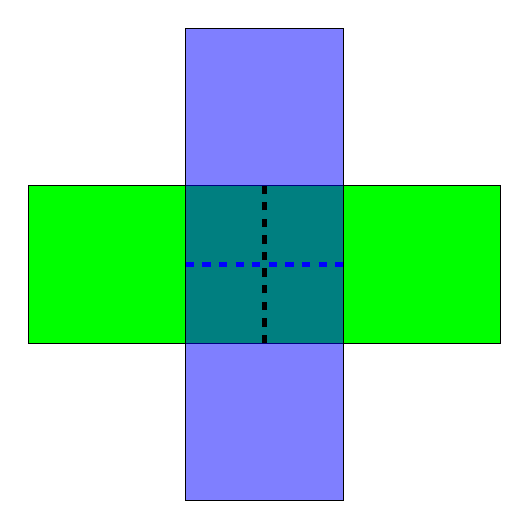
\begin{tikzpicture}
\filldraw[fill=green] (0,0) rectangle (6,2);
\filldraw[fill=blue, fill opacity=0.5] (2,-2) rectangle (4,4);
\draw[ultra thick, black, dashed] (3,0)--(3,2);
\draw[ultra thick, blue, dashed] (2,1)--(4,1);
\end{tikzpicture}
\caption[Lining up Crossings]{Lining up crossings. The green strand has the vertical running stitch marker, and the blue strand has the horizontal running stitch marker}
\end{figure}

Use a safety pin to attach the top and bottom strands until they can be permanently secured together. The start and end of each strand will be cross underneath another strand, to hide the join. Pin these to either side of the marker for their crossing. You can stitch the two ends together using the tail left over when you broke the yarn.

Alternately, for a stitched border, you can pin your piece flat as if you were blocking it.

Unless you change the dimensions to have extra wide strands, the knot will not hold its shape on its own. You'll have to secure the crossings in some manner. Several methods are given below. All of them make the fastenings essentially invisible, giving the impression that the knot is simply woven together.

\subsection*{Option 1: No Border} Using a tapestry needle and the same yarn the knot is made of, put a stitch through both strands at each crossing. Make sure it is not noticeable from the top. On the wrong side of the knot, stitch along the strand until you come to the next crossing, and repeat the process.

This gives loose connections, allowing the knot to flex when the piece is moved. It can (but doesn't have to) be used together with the other options as a kind of basting before the borders are added.

\subsection*{Option 2: Slip-stitch border} Using a contrasting colour yarn, and starting on a portion of a strand that is hidden under a crossing, slip-stitch along the chain end of each strand. Do this part before the knot is assembled, but do lay the knot out so you're sure you're stitching on the right side of each strand.

Assemble the knot, pinning or basting each crossing in place. Starting at an underneath crossing, slip stitch along the last row you worked, all around each strand.  Keep the yarn on the wrong side of the piece as you stitch from the right side. When you come to a crossing where the current strand is on top, work your stitches through both strands. When you come to a crossing where the current strand is on the bottom, work only through that strand.

This holds the pieces together very tightly, so it's important to make sure your intersections are lined up exactly how you want them. The front is quite pretty, but the back less so. This is a good option for  doilies and table runners that will sit flat, or lace that will be permanently sewn down.

\subsection*{Option 3: Stitched Border}
Using variations on blanket stitches and whip stitches, you can stitch along both edges of each strand once the piece is assembled and pinned into place. When the current strand crosses over another strand, pick up a few threads of yarn from the bottom strand in order to invisibly fasten the two strands together.

Keeping the strands positioned correctly is easier in this method than in Option 2. This method also differs from Option 2 by producing a two-sided finish. This is a good option for scarves or afghan squares, where both sides are likely to be seen.



%%%%%%%%%%%%%%%%%%%%%%%%%%
\section{\RK}
The \rk~is made up of two identical strands. Below are the stitching instructions, to be read as in \ref{sec:reading}. 

The finished dimensions are roughly 80 stitches wide by 30 stitches high. In crochet cotton, it is about the size of a bookmark; with medium yarn and a 4mm hook, it's a good size for a trivet.
%%%%%%%%%%%%%%%%%%%%%%%%%%
\begin{figure}[H]
\centering
\includegraphics{rectangle}
\caption[\RK]{\RK\gen}
\label{fig:gen1}
\end{figure}
Make \textbf{two copies} of the strand below. 
%\begin{description}
%\item[Foundation Chain:]
%10 \ch \m{2T}
%3 \ch / 7 \ch / 3 \ch \m{3B}
%3 \ch / 7 \ch / 3 \ch \m{4T}
%3 \ch / 7 \ch / 3 \ch \m{2B}
%10 \ch \m{1T}
%10 \ch \m{4B}
%3 \ch / 15 \ch / 3 \ch \m{5T}
%10 \ch \m{6B}
%10 \ch /  14 \ch /  10 \m{7T}
%3 \ch / 15 \ch / 3 \ch \m{5B}
%10 \ch /  14 \ch /  10 \m{6T}
%10 \ch \m{7B}
%3 \ch / 15 \ch / 3 \ch \m{3T}
%10 \ch
%\item[Row 1:]
%10 \sc /
%3 \sc / 14 \sc (-1) / 3 \sc /
%10 \sc /
%9 \sc (-1) /  5 sc, 2 dec sts, 5 sc /  9 \sc (-1) /
%3 \sc / 14 \sc (-1) / 3 \sc /
%9 \sc (-1) /  5 sc, 2 dec sts, 5 sc /  9 \sc (-1) /
%10 \sc /
%3 \sc / 14 \sc (-1) / 3 \sc /
%10 \sc /
%10 \sc /
%3 \sc / 8 \sc (+1) / 3 \sc /
%3 \sc / 8 \sc (+1) / 3 \sc /
%3 \sc / 8 \sc (+1) / 3 \sc /
%10 \sc 
%\item[Row 2:]
%10 \sc /
%3 \sc / 10 \sc (+2) / 3 \sc /
%3 \sc / 10 \sc (+2) / 3 \sc /
%3 \sc / 10 \sc (+2) / 3 \sc /
%10 \sc /
%10 \sc /
%3 \sc / 12 \sc (-2) / 3 \sc /
%10 \sc /
%9 \sc (-0) /  4 sc, 2 dec sts, 4 sc /  9 \sc (-0) /
%3 \sc / 12 \sc (-2) / 3 \sc /
%9 \sc (-0) /  4 sc, 2 dec sts, 4 sc /  9 \sc (-0) /
%10 \sc /
%3 \sc / 12 \sc (-2) / 3 \sc /
%10 \sc 
%\item[Row 3:]
%10 \sc /
%3 \sc / 11 \sc (-1) / 3 \sc /
%10 \sc /
%8 \sc (-1) /  3 sc, 2 dec sts, 3 sc /  8 \sc (-1) /
%3 \sc / 11 \sc (-1) / 3 \sc /
%8 \sc (-1) /  3 sc, 2 dec sts, 3 sc /  8 \sc (-1) /
%10 \sc /
%3 \sc / 11 \sc (-1) / 3 \sc /
%10 \sc /
%10 \sc /
%3 \sc / 11 \sc (+1) / 3 \sc /
%3 \sc / 11 \sc (+1) / 3 \sc /
%3 \sc / 11 \sc (+1) / 3 \sc /
%10 \sc 
%
%\item[Row 4:]
%10 \sc /
%3 \sc / 12 \sc (+1) / 3 \sc /
%3 \sc / 12 \sc (+1) / 3 \sc /
%3 \sc / 12 \sc (+1) / 3 \sc /
%10 \sc /
%10 \sc /
%3 \sc / 10 \sc (-1) / 3 \sc /
%10 \sc /
%7 \sc (-1) /  2 sc, 2 dec sts, 2 sc /  7 \sc (-1) /
%3 \sc / 10 \sc (-1) / 3 \sc /
%7 \sc (-1) /  2 sc, 2 dec sts, 2 sc /  7 \sc (-1) /
%10 \sc /
%3 \sc / 10 \sc (-1) / 3 \sc /
%10 \sc 
%\item[Row 5:]
%10 \sc /
%3 \sc / 8 \sc (-2) / 3 \sc /
%10 \sc /
%6 \sc (-1) /  1 sc, 2 dec sts, 1 sc /  6 \sc (-1) /
%3 \sc / 8 \sc (-2) / 3 \sc /
%6 \sc (-1) /  1 sc, 2 dec sts, 1 sc /  6 \sc (-1) /
%10 \sc /
%3 \sc / 8 \sc (-2) / 3 \sc /
%10 \sc /
%10 \sc /
%3 \sc / 14 \sc (+2) / 3 \sc /
%3 \sc / 14 \sc (+2) / 3 \sc /
%3 \sc / 14 \sc (+2) / 3 \sc /
%10 \sc 
%\item[Row 6:]
%10 \sc /
%3 \sc / 15 \sc (+1) / 3 \sc /
%3 \sc / 15 \sc (+1) / 3 \sc /
%3 \sc / 15 \sc (+1) / 3 \sc /
%10 \sc /
%10 \sc /
%3 \sc / 7 \sc (-1) / 3 \sc /
%10 \sc /
%6 \sc (-0) /2 dec sts /  6 \sc (-0) /
%3 \sc / 7 \sc (-1) / 3 \sc /
%6 \sc (-0) /   2 dec sts /  6 \sc (-0) /
%10 \sc /
%3 \sc / 7 \sc (-1) / 3 \sc /
%10 \sc 
%\end{description}
\begin{description}
\item[Foundation Chain:]
10 \ch \m{1T}
3 \ch / 7 \ch / 3 \ch \m{2B}
10 \ch \m{3T}
6 \ch /  2 \ch /  6 \m{4B}
3 \ch / 7 \ch / 3 \ch \m{2T}
6 \ch /  2 \ch /  6 \m{3B}
10 \ch \m{4T}
3 \ch / 7 \ch / 3 \ch \m{5B}
10 \ch \m{6T}
10 \ch \m{7B}
3 \ch / 15 \ch / 3 \ch \m{5T}
3 \ch / 15 \ch / 3 \ch \m{1B}
3 \ch / 15 \ch / 3 \ch \m{7T}
10 \ch 
\item[Row 1:]
10 \sc~ \m{}
3 \sc~ / 14 \sc~(-1) / 3 \sc~ \m{}
3 \sc~ / 14 \sc~(-1) / 3 \sc~ \m{}
3 \sc~ / 14 \sc~(-1) / 3 \sc~ \m{}
10 \sc~ \m{}
10 \sc~ \m{}
3 \sc~ / 8 \sc~(+1) / 3 \sc~ \m{}
10 \sc~ \m{}
7 \sc~(+1) /  1 sc, 2 ch, 1 sc /  7 \sc~(+1) \m{}
3 \sc~ / 8 \sc~(+1) / 3 \sc~ \m{}
7 \sc~(+1) /  1 sc, 2 ch, 1 sc /  7 \sc~(+1) \m{}
10 \sc~ \m{}
3 \sc~ / 8 \sc~(+1) / 3 \sc~ \m{}
10 \sc~ 
\item[Row 2:]
10 \sc~ \m{}
3 \sc~ / 10 \sc~(+2) / 3 \sc~ \m{}
10 \sc~ \m{}
7 \sc~ /  2 sc, 2 ch, 2 sc /  7 \sc~ \m{}
3 \sc~ / 10 \sc~(+2) / 3 \sc~ \m{}
7 \sc~ /  2 sc, 2 ch, 2 sc /  7 \sc~ \m{}
10 \sc~ \m{}
3 \sc~ / 10 \sc~(+2) / 3 \sc~ \m{}
10 \sc~ \m{}
10 \sc~ \m{}
3 \sc~ / 12 \sc~(-2) / 3 \sc~ \m{}
3 \sc~ / 12 \sc~(-2) / 3 \sc~ \m{}
3 \sc~ / 12 \sc~(-2) / 3 \sc~ \m{}
10 \sc~ 
\item[Row 3:]
10 \sc~ \m{}
3 \sc~ / 11 \sc~(-1) / 3 \sc~ \m{}
3 \sc~ / 11 \sc~(-1) / 3 \sc~ \m{}
3 \sc~ / 11 \sc~(-1) / 3 \sc~ \m{}
10 \sc~ \m{}
10 \sc~ \m{}
3 \sc~ / 11 \sc~(+1) / 3 \sc~ \m{}
10 \sc~ \m{}
8 \sc~(+1) /  3 sc, 2 ch, 3 sc /  8 \sc~(+1) \m{}
3 \sc~ / 11 \sc~(+1) / 3 \sc~ \m{}
8 \sc~(+1) /  3 sc, 2 ch, 3 sc /  8 \sc~(+1) \m{}
10 \sc~ \m{}
3 \sc~ / 11 \sc~(+1) / 3 \sc~ \m{}
10 \sc~ 
\item[Row 4:]
10 \sc~ \m{}
3 \sc~ / 12 \sc~(+1) / 3 \sc~ \m{}
10 \sc~ \m{}
9 \sc~(+1) /  4 sc, 2 ch, 4 sc /  9 \sc~(+1) \m{}
3 \sc~ / 12 \sc~(+1) / 3 \sc~ \m{}
9 \sc~(+1) /  4 sc, 2 ch, 4 sc /  9 \sc~(+1) \m{}
10 \sc~ \m{}
3 \sc~ / 12 \sc~(+1) / 3 \sc~ \m{}
10 \sc~ \m{}
10 \sc~ \m{}
3 \sc~ / 10 \sc~(-1) / 3 \sc~ \m{}
3 \sc~ / 10 \sc~(-1) / 3 \sc~ \m{}
3 \sc~ / 10 \sc~(-1) / 3 \sc~ \m{}
10 \sc~ 
\item[Row 5:]
10 \sc~ \m{}
3 \sc~ / 8 \sc~(-2) / 3 \sc~ \m{}
3 \sc~ / 8 \sc~(-2) / 3 \sc~ \m{}
3 \sc~ / 8 \sc~(-2) / 3 \sc~ \m{}
10 \sc~ \m{}
10 \sc~ \m{}
3 \sc~ / 14 \sc~(+2) / 3 \sc~ \m{}
10 \sc~ \m{}
9 \sc~ /  5 sc, 2 ch, 5 sc /  9 \sc~ \m{}
3 \sc~ / 14 \sc~(+2) / 3 \sc~ \m{}
9 \sc~ /  5 sc, 2 ch, 5 sc /  9 \sc~ \m{}
10 \sc~ \m{}
3 \sc~ / 14 \sc~(+2) / 3 \sc~ \m{}
10 \sc~ 
\item[Row 6:]
10 \sc~ \m{}
3 \sc~ / 15 \sc~(+1) / 3 \sc~ \m{}
10 \sc~ \m{}
10 \sc~(+1) /  6 sc, 2 ch, 6 sc /  10 \sc~(+1) \m{}
3 \sc~ / 15 \sc~(+1) / 3 \sc~ \m{}
10 \sc~(+1) /  6 sc, 2 ch, 6 sc /  10 \sc~(+1) \m{}
10 \sc~ \m{}
3 \sc~ / 15 \sc~(+1) / 3 \sc~ \m{}
10 \sc~ \m{}
10 \sc~ \m{}
3 \sc~ / 7 \sc~(-1) / 3 \sc~ \m{}
3 \sc~ / 7 \sc~(-1) / 3 \sc~ \m{}
3 \sc~ / 7 \sc~(-1) / 3 \sc~ \m{}
10 \sc~ 
\item[Finish] In border colour, slip stitch across the last row.
\end{description}
Lay out the knot to identify the right and wrong sides of each strand. Remember the start and end of a strand will join together underneath a crossing.

Assemble the two strands together, with crossings as in Figure~\ref{fig:crossRK} below.  Slip stitch along the remaining edges of both strands. When a strand is on top in an intersection, slip stitch through both strands to fasten them together. Running stitch markers at intersections should be perpendicular to one another.
%\begin{figure}[H]\centering
%\scalebox{1.4}{\begin{tikzpicture}
%\draw (0,0) node{\includegraphics[width=12cm]{rectangle}};
%%intersection: {x}{y}{label}
%\smintersection{1}{0}{1}
%\smintersection{-1}{0}{1}
%\smintersection{0}{1}{2}
%\smintersection{0}{-1}{2}
%\smintersection{2}{1}{3}
%\smintersection{-2}{-1}{3}
%\smintersection{-2}{1}{4}
%\smintersection{2}{-1}{4}
%\smintersection{-4}{1}{5}
%\smintersection{4}{-1}{5}
%\smintersection{4}{1}{7}
%\smintersection{-4}{-1}{7}
%\smintersection{5}{0}{6}
%\smintersection{-5}{0}{6}
%\end{tikzpicture}}
%\caption[Intersection labels for \rk]{Intersection labels for \rk \gen}\label{fig:crossRK}
%\end{figure}

%%%%%%%%%%%%
\begin{figure}[H]\centering
\scalebox{1.4}{\begin{tikzpicture}
\draw (0,0) node{\includegraphics[width=12cm]{rectangle}};

\foreach \r in {0,180}{
	\begin{scope}[rotate=\r]
	\smintersection{2}{1}{1}
	\smintersection{4}{1}{2}
	\smintersection{5}{0}{3}
	\smintersection{4}{-1}{4}
	\smintersection{2}{-1}{5}
	\smintersection{1}{0}{6}
	\smintersection{0}{1}{7}
	\end{scope}}
\end{tikzpicture}}
\caption[Intersection labels for \rk]{Intersection labels for \rk \gen}\label{fig:crossRK}
\end{figure}

The assembly of this knot is very similar to the \bk, so the gallery in Section~\ref{sec:gallery} may be useful for seeing how the various steps look.
%%%%%%%%%%%%
%pattern=["S","IQ","S","IP","IQ","IP","S","IQ","S","S","OQ","OQ","OQ","S"]
%markers=["1T","2B","3T","4B","2T","3B","4T","5B","6T","7B","5T","1B","7T"]
%%%%%%%%%%%%

%
%
%%%%%%%%%%%%%%%%%%%%%%%%%%%
%\section{\SK}
%%%%%%%%%%%%%%%%%%%%%%%%%%%
%The finished dimensions of this knot are about 50 stitches on each side. With a 4mm hook and aran yarn, it's a good size for a large trivet.
%\begin{figure}[H]\centering
%\includegraphics{square}
%\caption[\SK]{\SK \gen}\label{fig:gen2}
%\end{figure}
%
%Make \textbf{four copies} of the strand described below. For each of the four pieces, you'll need 19 running stitch markers, 9 of which are labelled.
%
%
%\begin{description}
%\item[Foundation Chain]
%10 \ch \m{2T}
%10 \ch \m{3B}
%6 \ch /  2 \ch /  6 \m{4T}
%3 \ch / 15 \ch / 3 \ch \m{5B}
%3 \ch / 7 \ch / 3 \ch \m{3T}
%10 \ch \m{4B}
%3 \ch / 7 \ch / 3 \ch \m{5T}
%10 \ch \m{2B}
%3 \ch / 7 \ch / 3 \ch \m{1T}
%10 \ch
%\item[Row 1:]
%10 \sc /
%3 \sc / 8 \sc (+1) / 3 \sc /
%10 \sc /
%3 \sc / 8 \sc (+1) / 3 \sc /
%10 \sc /
%3 \sc / 8 \sc (+1) / 3 \sc /
%3 \sc / 14 \sc (-1) / 3 \sc /
%6 \sc (+0) /  1 sc, 2 ch, 1 sc /  6 \sc (+0) /
%10 \sc /
%10 \sc 
%\item[Row 2:]
%10 \sc /
%10 \sc /
%7 \sc (+1) /  2 sc, 2 ch, 2 sc /  7 \sc (+1) /
%3 \sc / 12 \sc (-2) / 3 \sc /
%3 \sc / 10 \sc (+2) / 3 \sc /
%10 \sc /
%3 \sc / 10 \sc (+2) / 3 \sc /
%10 \sc /
%3 \sc / 10 \sc (+2) / 3 \sc /
%10 \sc 
%\item[Row 3:]
%10 \sc /
%3 \sc / 11 \sc (+1) / 3 \sc /
%10 \sc /
%3 \sc / 11 \sc (+1) / 3 \sc /
%10 \sc /
%3 \sc / 11 \sc (+1) / 3 \sc /
%3 \sc / 11 \sc (-1) / 3 \sc /
%8 \sc (+1) /  3 sc, 2 ch, 3 sc /  8 \sc (+1) /
%10 \sc /
%10 \sc 
%\item[Row 4:]
%10 \sc /
%10 \sc /
%9 \sc (+1) /  4 sc, 2 ch, 4 sc /  9 \sc (+1) /
%3 \sc / 10 \sc (-1) / 3 \sc /
%3 \sc / 12 \sc (+1) / 3 \sc /
%10 \sc /
%3 \sc / 12 \sc (+1) / 3 \sc /
%10 \sc /
%3 \sc / 12 \sc (+1) / 3 \sc /
%10 \sc 
%\item[Row 5:]
%10 \sc /
%3 \sc / 14 \sc (+2) / 3 \sc /
%10 \sc /
%3 \sc / 14 \sc (+2) / 3 \sc /
%10 \sc /
%3 \sc / 14 \sc (+2) / 3 \sc /
%3 \sc / 8 \sc (-2) / 3 \sc /
%9 \sc (+0) /  5 sc, 2 ch, 5 sc /  9 \sc (+0) /
%10 \sc /
%10 \sc 
%\item[Row 6:]
%10 \sc /
%10 \sc /
%10 \sc (+1) /  6 sc, 2 ch, 6 sc /  10 \sc (+1) /
%3 \sc / 7 \sc (-1) / 3 \sc /
%3 \sc / 15 \sc (+1) / 3 \sc /
%10 \sc /
%3 \sc / 15 \sc (+1) / 3 \sc /
%10 \sc /
%3 \sc / 15 \sc (+1) / 3 \sc /
%10 \sc 
%\end{description}
%Once you've made four copies, assemble them according to the diagram below in Figure~\ref{fig:SKint}. Pin them in place, then whip stitch around both sides of each strand.
%%as described in Section~\ref{sec:assembly}.
%
%\begin{figure}[H]\centering
%\scalebox{1.5}{\begin{tikzpicture}
%\draw (0,0)node{\includegraphics[width=8cm]{square}};
%
%\foreach \r in {0,90,180,270}{
%\begin{scope}[rotate=\r]
%\smintersection{2}{1}{2}
%\smintersection{3}{2}{3}
%\smintersection{2}{3}{4}
%\smintersection{0}{3}{5}
%\smintersection{-2}{3}{3}
%\smintersection{-3}{2}{4}
%\smintersection{-3}{0}{5}
%\smintersection{-2}{-1}{2}
%\smintersection{0}{-1}{1}\end{scope}}
%\end{tikzpicture}}
%\caption[Labelled Intersections for \SK ]{Labelled Intersections for \SK \gen}\label{fig:SKint}
%\end{figure}




%\fbox{original} Quarter turns have no straight segments
%For an afghan square?
%



%pattern=["S","S","IP","OQ","IQ","S","IQ","S","IQ","S"]

%Markers: 2T, 3B, x x ,4T, 5B, 3T, 4B, 5T, 2B, 1T
%
%
%***** Foundation Chain *****
%10 \ch /
%10 \ch /
%6 \ch /  2 \ch /  6 \ch / 
%20 \ch /
%12 \ch /
%10 \ch /
%12 \ch /
%10 \ch /
%12 \ch /
%10 \ch /
%
%***** Row 1 *****
%10 \sc /
%13 \sc ( + 1 ) /
%10 \sc /
%13 \sc ( + 1 ) /
%10 \sc /
%13 \sc ( + 1 ) /
%18 \sc ( - 2 ) /
%7 sc ( + 1 ) /  1 sc, 2 ch, 1 sc /  7 sc ( + 1 ) /
%10 \sc /
%10 \sc /
%
%***** Row 2 *****
%10 \sc /
%10 \sc /
%7 sc ( + 0 ) /  2 sc, 2 ch, 2 sc /  7 sc ( + 0 ) /
%17 \sc ( - 1 ) /
%14 \sc ( + 1 ) /
%10 \sc /
%14 \sc ( + 1 ) /
%10 \sc /
%14 \sc ( + 1 ) /
%10 \sc /
%
%***** Row 3 *****
%10 \sc /
%16 \sc ( + 2 ) /
%10 \sc /
%16 \sc ( + 2 ) /
%10 \sc /
%16 \sc ( + 2 ) /
%16 \sc ( - 1 ) /
%8 sc ( + 1 ) /  3 sc, 2 ch, 3 sc /  8 sc ( + 1 ) /
%10 \sc /
%10 \sc /
%
%***** Row 4 *****
%10 \sc /
%10 \sc /
%9 sc ( + 1 ) /  4 sc, 2 ch, 4 sc /  9 sc ( + 1 ) /
%14 \sc ( - 2 ) /
%17 \sc ( + 1 ) /
%10 \sc /
%17 \sc ( + 1 ) /
%10 \sc /
%17 \sc ( + 1 ) /
%10 \sc /
%
%***** Row 5 *****
%10 \sc /
%18 \sc ( + 1 ) /
%10 \sc /
%18 \sc ( + 1 ) /
%10 \sc /
%18 \sc ( + 1 ) /
%13 \sc ( - 1 ) /
%9 sc ( + 0 ) /  5 sc, 2 ch, 5 sc /  9 sc ( + 0 ) /
%10 \sc /
%10 \sc /
%
%***** Row 6 *****
%10 \sc /
%10 \sc /
%10 sc ( + 1 ) /  6 sc, 2 ch, 6 sc /  10 sc ( + 1 ) /
%12 \sc ( - 1 ) /
%20 \sc ( + 2 ) /
%10 \sc /
%20 \sc ( + 2 ) /
%10 \sc /
%20 \sc ( + 2 ) /
%10 \sc /

%%%%%%%%%%%%%%%%%%%%%%%%%%
\section{\BK}
%%%%%%%%%%%%%%%%%%%%%%%%%%
This knot is made up of repeating segments, so it can be worked as long as you like. Its finished height is about 30 stitches.

It could make a table runner, or decorative lace to sew to a hem. Because the edges of the knot are open, it twists easily, making it a difficult choice for a scarf or any other item that isn't usually laying flat.



\begin{figure}[H]\centering
\includegraphics[width=\linewidth]{border2}
\caption[\BK]{\BK\gen}\label{fig:gen3}
\end{figure}


%-----------------------------------

\subsection*{End Parts: Make $2$}
\begin{description}
\item[Foundation Chain:]
10 \ch \m{3T}
6 \ch /  2 \ch /  6 \m{2B}
10 \ch \m{1T}
3 \ch / 7 \ch / 3 \ch \m{7B}
10 \ch / 17 \ch / 10 \m{7T}
10 \ch 
\item[Row 1:]
10 \sc~ \m{}
9 \sc~ (-1)  /  14 \sc~ (-3)  /  9 \sc~(-1) \m{}
3 \sc~ / 8 \sc~(+1) / 3 \sc~ \m{}
10 \sc~ \m{}
7 \sc~(+1) /  1 sc, 2 ch, 1 sc /  7 \sc~(+1) \m{}
10 \sc~ 
\item[Row 2:]
10 \sc~ \m{}
7 \sc~ /  2 sc, 2 ch, 2 sc /  7 \sc~ \m{}
10 \sc~ \m{}
3 \sc~ / 10 \sc~(+2) / 3 \sc~ \m{}
9 \sc~   /  12 \sc~ (-2)  /  9 \sc~ \m{}
10 \sc~ 
\item[Row 3:]
10 \sc~ \m{}
8 \sc~ (-1)  /  9 \sc~ (-3)  /  8 \sc~(-1) \m{}
3 \sc~ / 11 \sc~(+1) / 3 \sc~ \m{}
10 \sc~ \m{}
8 \sc~(+1) /  3 sc, 2 ch, 3 sc /  8 \sc~(+1) \m{}
10 \sc~ 
\item[Row 4:]
10 \sc~ \m{}
9 \sc~(+1) /  4 sc, 2 ch, 4 sc /  9 \sc~(+1) \m{}
10 \sc~ \m{}
3 \sc~ / 12 \sc~(+1) / 3 \sc~ \m{}
7 \sc~ (-1)  /  7 \sc~ (-2)  /  7 \sc~(-1) \m{}
10 \sc~ 
\item[Row 5:]
10 \sc~ \m{}
7 \sc~   /  4 \sc~ (-3)  /  7 \sc~ \m{}
3 \sc~ / 14 \sc~(+2) / 3 \sc~ \m{}
10 \sc~ \m{}
9 \sc~ /  5 sc, 2 ch, 5 sc /  9 \sc~ \m{}
10 \sc~ 
\item[Row 6:]
10 \sc~ \m{}
10 \sc~(+1) /  6 sc, 2 ch, 6 sc /  10 \sc~(+1) \m{}
10 \sc~ \m{}
3 \sc~ / 15 \sc~(+1) / 3 \sc~ \m{}
6 \sc~ (-1)  /  2 \sc~ (-2)  /  6 \sc~(-1) \m{}
10 \sc~ 
\item[Finish] slip stitch along the last row in the border colour
\end{description}
%\begin{description}
%\item[Foundation Chain:]
%10 \ch \m{*T}
%6 \ch /  2 \ch /  6 \m{*B}
%10 \ch \m{*T}
%3 \ch / 7 \ch / 3 \ch \m{12B}
%10 \ch /  17 \ch /  10 \m{12T}
%10 \ch 
%\item[Row 1:]
%10 \sc /
%9 \sc~(-1)  /  15 \sc~(-2)  /  9 \sc~(-1) /
%3 \sc / 8 \sc~(+1) / 3 \sc /
%10 \sc /
%6 \sc~ /  1 sc, 2 ch, 1 sc /  6 \sc~  /
%10 \sc 
%\item[Row 2:]
%10 \sc /
%7 \sc~(+1) /  2 sc, 2 ch, 2 sc /  7 \sc~(+1)  /
%10 \sc /
%3 \sc / 10 \sc~(+2) / 3 \sc /
%9 \sc~  /  12 \sc~(-3)  /  9 \sc~ /
%10 \sc 
%\item[Row 3:]
%10 \sc /
%8 \sc~(-1)  /  9 \sc~(-3)  /  8 \sc~(-1) /
%3 \sc / 11 \sc~(+1) / 3 \sc /
%10 \sc /
%8 \sc~(+1) /  3 sc, 2 ch, 3 sc /  8 \sc~(+1)  /
%10 \sc 
%\item[Row 4:]
%10 \sc /
%9 \sc~(+1) /  4 sc, 2 ch, 4 sc /  9 \sc~(+1)  /
%10 \sc /
%3 \sc / 12 \sc~(+1) / 3 \sc /
%7 \sc~(-1)  /  6 \sc~(-3)  /  7 \sc~(-1) /
%10 \sc 
%\item[Row 5:]
%10 \sc /
%6 \sc~(-1)  /  4 \sc~(-2)  /  6 \sc~(-1) /
%3 \sc / 14 \sc~(+2) / 3 \sc /
%10 \sc /
%9 \sc~ /  5 sc, 2 ch, 5 sc /  9 \sc~  /
%10 \sc 
%\item[Row 6:]
%10 \sc /
%10 \sc~(+1) /  6 sc, 2 ch, 6 sc /  10 \sc~(+1)  /
%10 \sc /
%3 \sc / 15 \sc~(+1) / 3 \sc /
%6 \sc~  /  2 \sc~(-2)  /  6 \sc~ /
%10 \sc 
%\end{description}

%-----------------------------------


\subsection*{Oval Part: make $N$}
Make as many as you need to reach your desired length.

\begin{description}
\item[Foundation Chain:]
10 \ch \m{2T}
6 \ch /  2 \ch /  6 \m{1B}
10 \ch \m{4T}
10 \ch \m{3B}
10 \ch \m{2T}
6 \ch /  2 \ch /  6 \m{1B}
10 \ch \m{4T}
10 \ch 
\item[Row 1:]
10 \sc~ \m{}
10 \sc~ \m{}
7 \sc~(+1) /  1 sc, 2 ch, 1 sc /  7 \sc~(+1) \m{}
10 \sc~ \m{}
10 \sc~ \m{}
10 \sc~ \m{}
7 \sc~(+1) /  1 sc, 2 ch, 1 sc /  7 \sc~(+1) \m{}
10 \sc~ 
\item[Row 2:]
10 \sc~ \m{}
7 \sc~ /  2 sc, 2 ch, 2 sc /  7 \sc~ \m{}
10 \sc~ \m{}
10 \sc~ \m{}
10 \sc~ \m{}
7 \sc~ /  2 sc, 2 ch, 2 sc /  7 \sc~ \m{}
10 \sc~ \m{}
10 \sc~ 
\item[Row 3:]
10 \sc~ \m{}
10 \sc~ \m{}
8 \sc~(+1) /  3 sc, 2 ch, 3 sc /  8 \sc~(+1) \m{}
10 \sc~ \m{}
10 \sc~ \m{}
10 \sc~ \m{}
8 \sc~(+1) /  3 sc, 2 ch, 3 sc /  8 \sc~(+1) \m{}
10 \sc~ 
\item[Row 4:]
10 \sc~ \m{}
9 \sc~(+1) /  4 sc, 2 ch, 4 sc /  9 \sc~(+1) \m{}
10 \sc~ \m{}
10 \sc~ \m{}
10 \sc~ \m{}
9 \sc~(+1) /  4 sc, 2 ch, 4 sc /  9 \sc~(+1) \m{}
10 \sc~ \m{}
10 \sc~ 
\item[Row 5:]
10 \sc~ \m{}
10 \sc~ \m{}
9 \sc~ /  5 sc, 2 ch, 5 sc /  9 \sc~ \m{}
10 \sc~ \m{}
10 \sc~ \m{}
10 \sc~ \m{}
9 \sc~ /  5 sc, 2 ch, 5 sc /  9 \sc~ \m{}
10 \sc~ 
\item[Row 6:]
10 \sc~ \m{}
10 \sc~(+1) /  6 sc, 2 ch, 6 sc /  10 \sc~(+1) \m{}
10 \sc~ \m{}
10 \sc~ \m{}
10 \sc~ \m{}
10 \sc~(+1) /  6 sc, 2 ch, 6 sc /  10 \sc~(+1) \m{}
10 \sc~ \m{}
10 \sc~
 \item[Finish] slip stitch along the last row in the border colour
\end{description}

%\begin{description}
%\item[Foundation Chain:]
%10 \ch \m{1T}
%10 \ch \m{9B}
%6 \ch /  2 \ch /  6 \m{10T}
%10 \ch \m{11B}
%10 \ch \m{5T}
%10 \ch \m{8B}
%6 \ch /  2 \ch /  6 \m{7T}
%10 \ch 
%\item[Row 1:]
%10 \sc /
%6 \sc~ /  1 sc, 2 ch, 1 sc /  6 \sc~  /
%10 \sc /
%10 \sc /
%10 \sc /
%6 \sc~ /  1 sc, 2 ch, 1 sc /  6 \sc~  /
%10 \sc /
%10 \sc 
%\item[Row 2:]
%10 \sc /
%10 \sc /
%7 \sc~(+1) /  2 sc, 2 ch, 2 sc /  7 \sc~(+1)  /
%10 \sc /
%10 \sc /
%10 \sc /
%7 \sc~(+1) /  2 sc, 2 ch, 2 sc /  7 \sc~(+1)  /
%10 \sc 
%\item[Row 3:]
%10 \sc /
%8 \sc~(+1) /  3 sc, 2 ch, 3 sc /  8 \sc~(+1)  /
%10 \sc /
%10 \sc /
%10 \sc /
%8 \sc~(+1) /  3 sc, 2 ch, 3 sc /  8 \sc~(+1)  /
%10 \sc /
%10 \sc 
%\item[Row 4:]
%10 \sc /
%10 \sc /
%9 \sc~(+1) /  4 sc, 2 ch, 4 sc /  9 \sc~(+1)  /
%10 \sc /
%10 \sc /
%10 \sc /
%9 \sc~(+1) /  4 sc, 2 ch, 4 sc /  9 \sc~(+1)  /
%10 \sc 
%\item[Row 5:]
%10 \sc /
%9 \sc~ /  5 sc, 2 ch, 5 sc /  9 \sc~  /
%10 \sc /
%10 \sc /
%10 \sc /
%9 \sc~ /  5 sc, 2 ch, 5 sc /  9 \sc~  /
%10 \sc /
%10 \sc 
%\item[Row 6:]
%10 \sc /
%10 \sc /
%10 \sc~(+1) /  6 sc, 2 ch, 6 sc /  10 \sc~(+1)  /
%10 \sc /
%10 \sc /
%10 \sc /
%10 \sc~(+1) /  6 sc, 2 ch, 6 sc /  10 \sc~(+1)  /
%10 \sc 
%\end{description}
%-----------------------------------

\subsection*{Twisty Part: make $N-1$}
Make one fewer than you made of the last part.

\begin{description}
\item[Foundation Chain:]
10 \ch \m{1T}
10 \ch \m{2B}
10 \ch /  14 \ch /  10 \m{3T}
10 \ch \m{4B}
10 \ch \m{5T}
6 \ch / 2 \ch / 6 \m{5B}
10 \ch \m{6T}
10 \ch \m{5B}
10 \ch / 17 \ch / 10 \m{5T}
10 \ch \m{4B}
10 \ch \m{3T}
6 \ch /  2 \ch /  6 \m{2B}
10 \ch \m{1T}
10 \ch 
\item[Row 1:]
10 \sc~ \m{}
10 \sc~ \m{}
7 \sc~(+1) /  1 sc, 2 ch, 1 sc /  7 \sc~(+1) \m{}
10 \sc~ \m{}
10 \sc~ \m{}
9 \sc~ (-1)  /  14 \sc~ (-3)  /  9 \sc~(-1) \m{}
10 \sc~ \m{}
10 \sc~ \m{}
7 \sc~ (+1)  /  4 \sc~ (+2)  /  7 \sc~(+1) \m{}
10 \sc~ \m{}
10 \sc~ \m{}
9 \sc~(-1) /  5 sc, 2 dec sts, 5 sc /  9 \sc~(-1) \m{}
10 \sc~ \m{}
10 \sc~ 
\item[Row 2:]
10 \sc~ \m{}
10 \sc~ \m{}
9 \sc~ /  4 sc, 2 dec sts, 4 sc /  9 \sc~ \m{}
10 \sc~ \m{}
10 \sc~ \m{}
7 \sc~   /  7 \sc~ (+3)  /  7 \sc~ \m{}
10 \sc~ \m{}
10 \sc~ \m{}
9 \sc~   /  12 \sc~ (-2)  /  9 \sc~ \m{}
10 \sc~ \m{}
10 \sc~ \m{}
7 \sc~ /  2 sc, 2 ch, 2 sc /  7 \sc~ \m{}
10 \sc~ \m{}
10 \sc~ 
\item[Row 3:]
10 \sc~ \m{}
10 \sc~ \m{}
8 \sc~(+1) /  3 sc, 2 ch, 3 sc /  8 \sc~(+1) \m{}
10 \sc~ \m{}
10 \sc~ \m{}
8 \sc~ (-1)  /  9 \sc~ (-3)  /  8 \sc~(-1) \m{}
10 \sc~ \m{}
10 \sc~ \m{}
8 \sc~ (+1)  /  9 \sc~ (+2)  /  8 \sc~(+1) \m{}
10 \sc~ \m{}
10 \sc~ \m{}
8 \sc~(-1) /  3 sc, 2 dec sts, 3 sc /  8 \sc~(-1) \m{}
10 \sc~ \m{}
10 \sc~ 
\item[Row 4:]
10 \sc~ \m{}
10 \sc~ \m{}
7 \sc~(-1) /  2 sc, 2 dec sts, 2 sc /  7 \sc~(-1) \m{}
10 \sc~ \m{}
10 \sc~ \m{}
9 \sc~ (+1)  /  12 \sc~ (+3)  /  9 \sc~(+1) \m{}
10 \sc~ \m{}
10 \sc~ \m{}
7 \sc~ (-1)  /  7 \sc~ (-2)  /  7 \sc~(-1) \m{}
10 \sc~ \m{}
10 \sc~ \m{}
9 \sc~(+1) /  4 sc, 2 ch, 4 sc /  9 \sc~(+1) \m{}
10 \sc~ \m{}
10 \sc~ 
\item[Row 5:]
10 \sc~ \m{}
10 \sc~ \m{}
9 \sc~ /  5 sc, 2 ch, 5 sc /  9 \sc~ \m{}
10 \sc~ \m{}
10 \sc~ \m{}
7 \sc~   /  4 \sc~ (-3)  /  7 \sc~ \m{}
10 \sc~ \m{}
10 \sc~ \m{}
9 \sc~   /  14 \sc~ (+2)  /  9 \sc~ \m{}
10 \sc~ \m{}
10 \sc~ \m{}
7 \sc~ /  1 sc, 2 dec sts, 1 sc /  7 \sc~ \m{}
10 \sc~ \m{}
10 \sc~ 
\item[Row 6:]
10 \sc~ \m{}
10 \sc~ \m{}
6 \sc~(-1) /  0 sc, 2 dec sts, 0 sc /  6 \sc~(-1) \m{}
10 \sc~ \m{}
10 \sc~ \m{}
10 \sc~ (+1)  /  17 \sc~ (+3)  /  10 \sc~(+1) \m{}
10 \sc~ \m{}
10 \sc~ \m{}
6 \sc~ (-1)  /  2 \sc~ (-2)  /  6 \sc~(-1) \m{}
10 \sc~ \m{}
10 \sc~ \m{}
10 \sc~(+1) /  6 sc, 2 ch, 6 sc /  10 \sc~(+1) \m{}
10 \sc~ \m{}
10 \sc~ 
 \item[Finish] slip stitch along the last row in the border colour
 \end{description}

%\begin{description}
%\item[Foundation Chain:]
%10 \ch \m{2T}
%6 \ch /  2 \ch /  6 \m{2B}
%10 \ch \m{3T}
%10 \ch \m{4B}
%10 \ch /  17 \ch /  10 \m{4T}
%10 \ch \m{5B}
%10 \ch \m{6T}
%6 \ch /  2 \ch /  6 \m{7B}
%10 \ch \m{8T}
%10 \ch \m{3B}
%10 \ch \m{9T}
%10 \ch \m{10B}
%10 \ch /  14 \ch /  10 \m{11T}
%10 \ch 
%\item[Row 1:]
%10 \sc /
%9 \sc~(-1) /  5 sc, 2 dec sts, 5 sc /  9 \sc~(-1)  /
%10 \sc /
%10 \sc /
%10 \sc /
%10 \sc /
%6 \sc~ /  1 sc, 2 ch, 1 sc /  6 \sc~  /
%10 \sc /
%10 \sc /
%9 \sc~(-1)  /  15 \sc~(-2)  /  9 \sc~(-1) /
%10 \sc /
%10 \sc /
%6 \sc~  /  4 \sc~(+2)  /  6 \sc~ /
%10 \sc /
%\item[Row 2:]
%10 \sc /
%7 \sc~(+1)  /  6 \sc~(+2)  /  7 \sc~(+1) /
%10 \sc /
%10 \sc /
%9 \sc~  /  12 \sc~(-3)  /  9 \sc~ /
%10 \sc /
%10 \sc /
%7 \sc~(+1) /  2 sc, 2 ch, 2 sc /  7 \sc~(+1)  /
%10 \sc /
%10 \sc /
%10 \sc /
%10 \sc /
%9 \sc~ /  4 sc, 2 dec sts, 4 sc /  9 \sc~  /
%10 \sc /
%\item[Row 3:]
%10 \sc /
%8 \sc~(-1) /  3 sc, 2 dec sts, 3 sc /  8 \sc~(-1)  /
%10 \sc /
%10 \sc /
%10 \sc /
%10 \sc /
%8 \sc~(+1) /  3 sc, 2 ch, 3 sc /  8 \sc~(+1)  /
%10 \sc /
%10 \sc /
%8 \sc~(-1)  /  9 \sc~(-3)  /  8 \sc~(-1) /
%10 \sc /
%10 \sc /
%8 \sc~(+1)  /  9 \sc~(+3)  /  8 \sc~(+1) /
%10 \sc /
%\item[Row 4:]
%10 \sc /
%9 \sc~(+1)  /  12 \sc~(+3)  /  9 \sc~(+1) /
%10 \sc /
%10 \sc /
%7 \sc~(-1)  /  6 \sc~(-3)  /  7 \sc~(-1) /
%10 \sc /
%10 \sc /
%9 \sc~(+1) /  4 sc, 2 ch, 4 sc /  9 \sc~(+1)  /
%10 \sc /
%10 \sc /
%10 \sc /
%10 \sc /
%7 \sc~(-1) /  2 sc, 2 dec sts, 2 sc /  7 \sc~(-1)  /
%10 \sc /
%\item[Row 5:]
%10 \sc /
%6 \sc~(-1) /  1 sc, 2 dec sts, 1 sc /  6 \sc~(-1)  /
%10 \sc /
%10 \sc /
%10 \sc /
%10 \sc /
%9 \sc~ /  5 sc, 2 ch, 5 sc /  9 \sc~  /
%10 \sc /
%10 \sc /
%6 \sc~(-1)  /  4 \sc~(-2)  /  6 \sc~(-1) /
%10 \sc /
%10 \sc /
%9 \sc~  /  15 \sc~(+3)  /  9 \sc~ /
%10 \sc /
%\item[Row 6:]
%10 \sc /
%10 \sc~(+1)  /  17 \sc~(+2)  /  10 \sc~(+1) /
%10 \sc /
%10 \sc /
%6 \sc~  /  2 \sc~(-2)  /  6 \sc~ /
%10 \sc /
%10 \sc /
%10 \sc~(+1) /  6 sc, 2 ch, 6 sc /  10 \sc~(+1)  /
%10 \sc /
%10 \sc /
%10 \sc /
%10 \sc /
%6 \sc~ /  0 sc, 2 dec sts, 0 sc /  6 \sc~  /
%10 \sc /
%\end{description}

%Ovals:
%pattern=["S","IP","S","S","S","IP","S","S",]
%markers=["2T","1B","4T","3B","2T","1B","4T","end"]
%
%Twists:
%pattern=["S","S","OP","S","S","IT","S","S","OT","S","S","IP","S","S"]
%markers=["1T","2B","3T","4B","5T","5B","6T","5B","5T","4B","3T","2B","1T","end"]
%
%End Pieces:
%pattern=["S","IP","S","IQ","OT","S"]
%markers=["3T","2B","1T","7B","7T","end"]


%-----------------------------------
Lay out the knot according to the labels below.
\begin{figure}[H]\centering
\scalebox{1.4}{\begin{tikzpicture}
\draw(0,0)node{\includegraphics[width=12cm]{border2}};
\foreach \xshift in {0,3,-3}
	{
	\begin{scope}[xshift=\xshift cm]
	\smintersection {0}{0}{6}
	\foreach \r in {0,180}{
		\begin{scope}[rotate=\r]
		\smintersection {-.5}{.5}{1}
		\smintersection {-1}{1}{2}
		\smintersection {-1.5}{.5}{3}
		\smintersection {-1}{0}{4}
		\smintersection {-.5}{-.5}{5}
		\end{scope}}
	\end{scope}
	}
\foreach \r in {0,180}{
	\begin{scope}[rotate=\r]
		\smintersection{5}{0}{4}
		\smintersection{5.5}{0.5}{1}
		\smintersection{5}{1}{2}
		\smintersection{4.5}{0.5}{3}
		\smintersection{5.5}{-.5}{7}
	\end{scope}}\end{tikzpicture}}
\caption[Intersection labels for \bk]{Intersection labels for \bk \gen}\label{fig:gen4}
\end{figure}

Slip stitch along the foundation chains to finish and secure intersections.

%%%%%%%%%%%%%%%%%%%%%%%%%%
\section{\BK ~Gallery}\label{sec:gallery}
%%%%%%%%%%%%%%%%%%%%%%%%%%
The three types of parts are shown below. These are crocheted separately, with one slip-stitch row added before the pieces are assembled.
%%%%%%%%%%%%
\begin{figure}[H]\centering
\begin{subfigure}[t]{.45\textwidth}\centering
\includegraphics[width=.95\textwidth]{bk/end}
\caption{After sixth row}
\end{subfigure}
%
\begin{subfigure}[t]{.45\textwidth}
		\centering
		\includegraphics[width=.95\textwidth]{bk/end2}
\caption{After slip-stitch row}
\end{subfigure}
\caption{End part of \bk}
\end{figure}


%%%%%%%%%%%%%%%%%%%%%%%%
\begin{figure}[H]\centering
\begin{subfigure}[t]{.45\textwidth}\centering
\includegraphics[width=.95\textwidth]{bk/oval}
\caption{After sixth row}
\end{subfigure}
%
\begin{subfigure}[t]{.45\textwidth}
		\centering
		\includegraphics[width=.95\textwidth]{bk/oval2}
\caption{After slip-stitch row}
\end{subfigure}
\caption{Oval part of \bk}
\end{figure}
%%%%%%%%%%%%
%%%%%%%%%%%%
\begin{figure}[H]\centering
\begin{subfigure}[t]{.45\textwidth}\centering
\includegraphics[width=.95\textwidth]{bk/twist}
\caption{After sixth row}
\end{subfigure}
%
\begin{subfigure}[t]{.45\textwidth}
		\centering
		\includegraphics[width=.95\textwidth]{bk/twist2}
\caption{After slip-stitch row}
\end{subfigure}
\caption{Twisty part of \bk}
\end{figure}
%%%%%%%%%%%%

To work the slip-stitch row, start in the last sc of the last row of the piece, and use the border colour.


%%%%%%%%%%%%
\begin{figure}[H]\centering
\begin{subfigure}[t]{.3\textwidth}\centering
\includegraphics[width=.95\textwidth]{bk/slst1}
\caption{Push hook through the last sc of the last row}
\end{subfigure}
%
\begin{subfigure}[t]{.3\textwidth}
		\centering
		\includegraphics[width=.95\textwidth]{bk/slst2}
\caption{pull up a loop}
\end{subfigure}
%
\begin{subfigure}[t]{.3\textwidth}
		\centering
		\includegraphics[width=.95\textwidth]{bk/slst3}
\caption{slip stitch}
\end{subfigure}
\caption{Slip-stitch row}
\end{figure}
%%%%%%%%%%%%

Generally you'll be working one slst in each stitch, but sometimes at tight corners a little variation can make the piece look cleaner. At outside points, you can add one chain, and at inside corners you can slst2tog.


%%%%%%%%%%%%
\begin{figure}[H]\centering
\begin{subfigure}[t]{.3\textwidth}\centering
\includegraphics[width=.95\textwidth]{bk/slstcorner1}
\caption{You'll work a slst through both chains in the point}
\end{subfigure}
%
\begin{subfigure}[t]{.3\textwidth}
		\centering
		\includegraphics[width=.95\textwidth]{bk/slstcorner2}
\caption{Adding an extra chain between them makes a pointier finish}
\end{subfigure}
%
\begin{subfigure}[t]{.3\textwidth}
		\centering
		\includegraphics[width=.95\textwidth]{bk/inside}
\caption{On the inside of a point or twist, you can slst2tog to keep the curve tight}
\end{subfigure}
\caption{Slip stitching around a point}
\end{figure}
%%%%%%%%%%%%

Once two adjacent parts are made, you can weave them together and pin their intersections.


%%%%%%%%%%%%%%%%%%
\begin{figure}[H]
\centering
\includegraphics[width=.75\textwidth]{bk/line}
\caption{Line up running stitch markers so they are perpendicular}
\end{figure}
%%%%%%%%%



%%%%%%%%%%%%%%%%%%%%%%%%%%%%%%
\begin{figure}[H]\centering
\begin{subfigure}[t]{.45\textwidth}\centering
\includegraphics[width=.95\textwidth]{bk/weave1}
\caption{Front}
\end{subfigure}
%
\begin{subfigure}[t]{.45\textwidth}
		\centering
		\includegraphics[width=.95\textwidth]{bk/weave2}
\caption{Back}
\end{subfigure}
\caption{Intersections of end part and oval part pinned}
\end{figure}
%%%%%%%%%%%%

Once all intersections of a part are pinned, you can sew its ends together and slip stitch around its foundation chain. If you want to be quite fancy, you can work an invisible join for the slip stitches. Since this will only be seen by you (as it's hidden under a crossing) this is not crucial.


%%%%%%%%%%%%
\begin{figure}[H]\centering
\begin{subfigure}[t]{.3\textwidth}\centering
\includegraphics[width=.95\textwidth]{bk/join1}
\caption{After a part is woven, you'll sew its ends together}
\end{subfigure}
%
\begin{subfigure}[t]{.3\textwidth}
		\centering
		\includegraphics[width=.95\textwidth]{bk/join2}
\caption{Thread end of border yarn onto a tapestry needle}
\end{subfigure}
%
\begin{subfigure}[t]{.3\textwidth}
		\centering
		\includegraphics[width=.95\textwidth]{bk/join3}
\caption{Bring end underneath both legs of the first slip stitch}
\end{subfigure}

\begin{subfigure}[t]{.3\textwidth}\centering
\includegraphics[width=.95\textwidth]{bk/join4}
\caption{Pull through, snug but not tight}
\end{subfigure}
%
\begin{subfigure}[t]{.3\textwidth}
		\centering
		\includegraphics[width=.95\textwidth]{bk/join5}
\caption{Insert hook into the last sl st}
\end{subfigure}
%
\begin{subfigure}[t]{.3\textwidth}
		\centering
		\includegraphics[width=.95\textwidth]{bk/join6}
\caption{slip stitch}
\end{subfigure}
\caption{Invisible slst join (optional)}
\end{figure}
%%%%%%%%%%%%

Now you will finish the border and secure the intersections by adding a slip-stitch row along the foundation chain. Remember to only do this part after all intersections of a piece are pinned, otherwise the remaining intersection might be unsecured.


%%%%%%%%%%%%
\begin{figure}[H]\centering
\begin{subfigure}[t]{.45\textwidth}\centering
\includegraphics[width=.95\textwidth]{bk/top1}
\caption{Start where the strand will be hidden underneath a crossing}
\end{subfigure}
%
\begin{subfigure}[t]{.45\textwidth}
		\centering
		\includegraphics[width=.95\textwidth]{bk/top2}
\caption{Keeping your skein of yarn in the back of the piece, pull up a loop}
\end{subfigure}
\caption{Starting the slip-stich row along the foundation chain}
\end{figure}

%%%%%%%%%%%%

\begin{figure}[H]\centering
\begin{subfigure}[t]{.45\textwidth}\centering
\includegraphics[width=.95\textwidth]{bk/top5}
\caption{Slip stitch until you are 3 stitches away from the marker of the next crossing (which will be a top)}
\end{subfigure}
%
\begin{subfigure}[t]{.45\textwidth}
		\centering
		\includegraphics[width=.95\textwidth]{bk/top6}
\caption{Push your hook through both layers, picking up the bottom layer three rows above its own marker}
\end{subfigure}


\begin{subfigure}[t]{.45\textwidth}\centering
\includegraphics[width=.95\textwidth]{bk/top7}
\caption{Slip stitch through both layers, moving over one stitch on the top layer and one row on the bottom layer each time}
\end{subfigure}
%
\begin{subfigure}[t]{.45\textwidth}
		\centering
		\includegraphics[width=.95\textwidth]{bk/top8}
\caption{The back should look like this: a straight line, parallel to the bottom stitch marker}
\end{subfigure}

\caption{Stitching over a crossing}
\end{figure}
%%%%%%%%%%%%

In the next crossing, the strand you're working on will be on the bottom. Simply fold back the top and continue stitching through your strand only. If the top of this crossing has already been secured, you'll have to stitch around the ends, which only takes mild finagling.


%%%%%%%%%%%%
\begin{figure}[H]\centering
\begin{subfigure}[t]{.45\textwidth}\centering
\includegraphics[width=.95\textwidth]{bk/under1}
\caption{When you approach the next crossing, with the working strand on the bottom,}
\end{subfigure}
%
\begin{subfigure}[t]{.45\textwidth}
		\centering
		\includegraphics[width=.95\textwidth]{bk/under2}
\caption{it can be helpful to fold over the piece, so the bottom is easier to access}
\end{subfigure}
\caption{Bottom crossing}
\end{figure}
%%%%%%%%%%%%

In the pictures below, the end piece has been completely finished, while the oval piece has not yet had its last slip stitch row added.

%%%%%%%%%%%%
\begin{figure}[H]\centering
\begin{subfigure}[t]{.45\textwidth}\centering
\includegraphics[width=.95\textwidth]{bk/weave3}
\caption{Front}
\end{subfigure}
%
\begin{subfigure}[t]{.45\textwidth}
		\centering
		\includegraphics[width=.95\textwidth]{bk/weave4}
\caption{Back }
\end{subfigure}
\caption{End piece intersections secured with slip stitches along foundation row}
\end{figure}
%%%%%%%%%%%%


%%%%%%%%%%%%
\begin{figure}[H]\centering
\begin{subfigure}[t]{.45\textwidth}\centering
\includegraphics[width=.95\textwidth]{bk/done3}
\caption{Front}
\end{subfigure}
%
\begin{subfigure}[t]{.45\textwidth}
		\centering
		\includegraphics[width=.95\textwidth]{bk/done4}
\caption{Back}
\end{subfigure}
\caption{Finished \bk, markers removed}
\end{figure}
%%%%%%%%%%%%

\section{Knot specifications}
The strands' patterns and markers are given below, formatted for the program from Section~\ref{ssec:Python}. If you'd like to use the program to change some parameters of the knots, you can copy-paste the lists below.

\begin{description}
\item[\RK:]$ $\\
\texttt{ pattern=["S","IQ","S","IP","IQ","IP","S","IQ","S","S","OQ","OQ","OQ","S"]}\\
\texttt{markers=["1T","2B","3T","4B","2T","3B","4T","5B","6T","7B","5T","1B","7T"]}

\item[\BK:]$ $
\begin{description}
\item[End Parts:]$ $\\
\texttt{pattern=["S","IP","S","IQ","OT","S"]}\\
\texttt{markers=["3T","2B","1T","7B","7T"]}

\item[Oval Parts:]$ $\\
\texttt{pattern=["S","IP","S","S","S","IP","S","S",]}\\
\texttt{markers=["2T","1B","4T","3B","2T","1B","4T"]}

\item[Twisty Parts:]$ $\\
\texttt{pattern=["S","S","OP","S","S","IT","S","S","OT","S","S","IP","S","S"]}\\
\texttt{markers=["1T","2B","3T","4B","5T","5B","6T","5B","5T","4B","3T","2B","1T"]}

\end{description}
\end{description}


%%%%%%%%%%%%%%%%%%%%%%%%%%
%\section{Large Example Knot}
%%%%%%%%%%%%%%%%%%%%%%%%%%%
%[picture]
%
%This knot has 13 different pieces. The centre circle is Piece A, of which you will make one; then you will make four each of Pieces B, C, and D.
%
%The assembly diagram is [somewhere]
%%-----------------------------------
%\subsection*{Piece A: Make 1} %inner ring
%%pattern=["S","IQ","S","IQ","S","IQ","S","IQ"]
%
%8 segments, 7 markers: 1, 2, 1, 2, 1, 2, 1
%\begin{description}
%\item[Foundation Chain]
%10 ch \m{1}
%12 ch \m{2}
%10 ch \m{1}
%12 ch \m{2}
%10 ch \m{1}
%12 ch \m{2}
%10 ch \m{1}
%12 ch 
%\item[Row 1]
%*13 sc (+1) /
%10 sc /
%
%Repeat from * three more times (no marker after the last stitch of the row)
%
%\item[Row 2]
%* 10 sc /
%14 sc (+1) /
%
%Repeat from * three more times (no marker after the last stitch of the row)
%
%\item[Row 3]
% *
%16 sc (+2) /
%10 sc /
%
%Repeat from * three more times (no marker after the last stitch of the row)
%
%\item[Row 4] *
%10 sc /
%17 sc (+1) /
%
%Repeat from * three more times (no marker after the last stitch of the row)
%
%\item[Row 5] *
%18 sc (+1) /
%10 sc /
%
%Repeat from * three more times (no marker after the last stitch of the row)
%
%\item[Row 6]*
%10 sc /
%20 sc (+2) /
%
%Repeat from * three more times (no marker after the last stitch of the row)
%\end{description}
%
%%-----------------------------------
%%-----------------------------------
%\subsection*{Piece B: Make 4}%oval rings
%This piece has 10 segments, so set aside 9 running markers. When finished it will look like a boxy oval.
%
%%pattern=["S","IQ","IQ","S","S","S","IQ","IQ","S","S"]
%%S, IQ, IQ, S, S, S, IQ, IQ, S, S --fix pattern!
%
%%Markers: 3, 4, 5, 6, 7, 8, 9, 10, 11
%%-----------------------------------
%Markers: 3-11 (9 markers, 10 segments)
%
%\begin{description}
%\item[Foundation Chain] Work the following numbers of chain stitches, separated by labeled markers:
%
%10  \m{3}
%12  \m{4}
%12  \m{5}
%10  \m{6}
%10  \m{7}
%10  \m{8}
%12  \m{9}
%12  \m{10}
%10  \m{11}
%10  
%
%\item[Row 1] Work the following number of sc:
%
%10  /
%10  /
%13  (+1) /
%13  (+1) /
%10  /
%10  /
%10  /
%13  (+1) /
%13  (+1) /
%10  
%
%\item[Row 2]
%10  /
%14  (+1) /
%14  (+1) /
%10  /
%10  /
%10  /
%14  (+1) /
%14  (+1) /
%10  /
%10  
%
%\item[Row 3]
%10  /
%10  /
%16  (+2) /
%16  (+2) /
%10  /
%10  /
%10  /
%16  (+2) /
%16  (+2) /
%10  
%
%
%\item[Row 4]
%10  /
%17  (+1) /
%17  (+1) /
%10  /
%10  /
%10  /
%17  (+1) /
%17  (+1) /
%10  /
%10  
%
%\item[Row 5]
%10  /
%10  /
%18  (+1) /
%18  (+1) /
%10  /
%10  /
%10  /
%18  (+1) /
%18  (+1) /
%10  
%
%\item[Row 6]
%10  /
%20  (+2) /
%20  (+2) /
%10  /
%10  /
%10  /
%20  (+2) /
%20  (+2) /
%10  /
%10  
%\end{description}
%%
%%
%%
%%\begin{description}
%%\item[Foundation Chain] Work the following numbers of chain stitches:\\
%%10 \m{4} 12 \m{5} 12 \m{6} 10 \m{7} 10 \m{8} 12 \m{9} 12 \m{10} 10 
%%\item[Row 1] For the remaining six rows, work the following numbers of single crochets.\\
%%10 / 13  (+1) / 13  (+1) / 10 / 10 / 13  (+1) / 13  (+1) / 10 
%%\item[Row 2]
%%10 / 14 (+1) / 14  (+1) / 10 / 10 / 14  (+1) / 14  (+1) / 10 
%%\item[Row 3]
%%10 / 16  (+2) / 16  (+2) / 10 / 10 / 16  (+2) / 16  (+2) / 10  
%%\item[Row 4]
%%10 / 17  (+1)  / 17  (+1)  / 10 / 10 / 17  (+1) / 17  (+1) / 10 
%%\item[Row 5]
%%10 / 18  (+1) / 18  (+1) / 10 / 10 / 18  (+1) / 18  (+1) / 10 
%%\item[Row 6]
%%10 / 20  (+2)/ 20  (+2) / 10 / 10 / 20  (+2) / 20  (+2)  / 10 
%%\end{description}
%%-----------------------------------
%\subsection*{Piece C: Make 4}%figure 8
%%-----------------------------------
%This piece has 12 segments, so set aside 11 running markers. It has a figure-8 shape with one end pointy and one end round.
%
%%M: 8, 2, x, x, 1, 7, 12, 9, 13, 14, 10
%%pattern=["S","S","IP","S","IQ","S","OQ","OQ","OQ","S"]
%
%Markers: 10, 1xx, 2, 11, 12, 9, 13, 14, 8
%
%
%\begin{description}
%\item[Foundation Chain]
%Work the following number of chains:
%
%10 \ch \m{10}
%10 \ch \m{1}
%6 \ch / 2 \ch /  6 \ch \m{2}
%10 \ch \m{11}
%12 \ch \m{12}
%10 \ch \m{9}
%20 \ch \m{13}
%20 \ch \m{14}
%20 \ch \m{8}
%10 \ch 
%\item[Row 1]
%All stitches are sc unless specified otherwise
%
%10  /
%18  (-2) /
%18  (-2) /
%18  (-2) /
%10  /
%13  (+1) /
%10  /
%7  (+1) /  1 sc, 2 ch, 1 sc /  7 sc (+1) /
%10  /
%10  
%\item[Row 2]
%10  /
%10  /
%7   /  2 sc, 2 ch, 2 sc /  7   /
%10  /
%14  (+1) /
%10  /
%17  (-1) /
%17  (-1) /
%17  (-1) /
%10  
%\item[Row 3]
%10  /
%16  (-1) /
%16  (-1) /
%16  (-1) /
%10  /
%16  (+2) /
%10  /
%8  (+1) /  3 sc, 2 ch, 3 sc /  8  (+1) /
%10  /
%10  
%\item[Row 4]
%10  /
%10  /
%9  (+1) /  4 sc, 2 ch, 4 sc /  9  (+1) /
%10  /
%17  (+1) /
%10  /
%14  (-2) /
%14  (-2) /
%14  (-2) /
%10  
%\item[Row 5]
%10  /
%13  (-1) /
%13  (-1) /
%13  (-1) /
%10  /
%18  (+1) /
%10  /
%9  /  5 sc, 2 ch, 5 sc /  9  /
%10  /
%10  
%\item[Row 6]
%10  /
%10  /
%10  (+1) /  6 sc, 2 ch, 6 sc /  10  (+1) /
%10  /
%20  (+2) /
%10  /
%12  (-1) /
%12  (-1) /
%12  (-1) /
%10  
%\end{description}
%
%%\begin{description}
%%
%%\item[Foundation Chain] Work the following numbers of chain stitches:\\
%%10/ 10 /
%%%34
%%10 / 14 / 10
%%%
%% / 10 / 20 / 10 / 12 / 12 / 12 / 10 
%%\item[Row 1]
%%  10 sc / 13 sc (+1) / 13 sc (+1) / 13 sc (+1) /  10 sc / 18 sc (-2) / 10 sc /
%%9 sc (-1) /5 sc, 2 dec sts, 5 sc / 9 sc (-1) /
%%10 sc / 10 sc
%%\item[Row 2]
%%10 sc / 10 sc / 9 sc / 4 sc, 2 dec sts, 4 sc / 9 sc / 10 sc / 17 sc (-1) / 10 sc / 14 sc (+1) / 14 sc (+1) / 14 sc (+1) / 10 sc 
%%\item[Row 3]
%% 10 sc / 16 sc (+2) / 16 sc (+2) / 16 sc (+2) / 10 sc / 16 sc (-1) / 10 sc / 8 sc (-1) / 3 sc, 2 dec sts, 3 sc / 8 sc (-1) / 10 sc / 10 sc
%%\item[Row 4] 10 sc / 7 sc (-1) / 2 sc, 2 dec sts, 2 sc / 7 sc(-1) / 10 sc / 14 sc (-2) / 10sc / 10 sc / 17 sc (-1) / 17 sc (-1) / 17 sc (-1) / 10 sc 
%%\item[Row 5] 10 sc / 18 sc (+1) / 18 sc (+1) / 18 sc (+1) / 10 sc / 13 sc (-1) / 10 sc / 7 sc / 1 sc, 2 dec sts, 1 sc / 7 sc / 10 sc / 10 sc
%%\item[Row 6]
%% 10 sc / 10 sc / 6 sc (-1) / 2 dec sts / 6 sc (-1) / 10 sc / 12 sc (-1) / 10 sc / 20 sc (+2) / 20 sc (+2) / 20 sc (+2) / 10 sc 
%%\end{description}
%%-----------------------------------
%%\subsection*{\fbox{Piece D: Make 4}}%corner widgets
%\hrule
%\begin{center}
%Piece D: Make 4
%\end{center}
%\hrule
%%old %pattern=["IQ","S","S","OQ","S","S","IP","IQ","S","OQ","S","S","OP","S","S","S","IQ","S","IQ","OQ"]
%%pattern=["IQ","OQ","S","OQ","S","S","S","IP","S","S","IQ","S","OQ","OP","S","S","IQ","S","S","OQ"]
%
%
%
%M: 14, 15, 16, 17, 6, 18, 19, xx, 3, 20, 5, 17, 21, 15, xx, 16, 21, 7, 18, 20, 4
%%M: 4, 15, 16, 11, 13, 17, 18, x, x, 19, 17, 20, 3, 15, 5, x, x, 6, 16, 21, 20, 18, 19,  14
%
%
%%fix me 
%
%This is the most involved piece, but it uses all the same tricks as the pieces you've already made. It's just longer, with more self-crossings. Don't worry about making the crossings work out while you're crocheting it. You can arrange it all once it's done.
%
%There are 24 segments, so prepare 23 running stitch markers.
%
%\begin{description}
%\item[Foundation Chain] Work the following number of chain stitches, separated by stitch markers.\\
%12 \ch /
%20 \ch /
%10 \ch /
%20 \ch /
%10 \ch /
%10 \ch /
%10 \ch /
%6 \ch /  2 \ch /  6 \ch /
%10 \ch /
%10 \ch /
%12 \ch /
%10 \ch /
%20 \ch /
%10 \ch /  14 \ch /  10 \ch /
%10 \ch /
%10 \ch /
%12 \ch /
%10 \ch /
%10 \ch /
%20 \ch 
%\item[Row 1] All stitches are sc unless otherwise specified.\\
%18  (-2) /
%10  /
%10  /
%13  (+1) /
%10  /
%10  /
%9  (-1) /  5 sc, 2 dec sts, 5 sc /  9  (-1) /
%18  (-2) /
%10  /
%13  (+1) /
%10  /
%10  /
%7  (+1) /  1 sc, 2 ch, 1 sc /  7  (+1) /
%10  /
%10  /
%10  /
%18  (-2) /
%10  /
%18  (-2) /
%13  (+1) 
%\item[Row 2]
%14  (+1) /
%17  (-1) /
%10  /
%17  (-1) /
%10  /
%10  /
%10  /
%7   /  2 sc, 2 ch, 2 sc /  7   /
%10  /
%10  /
%14  (+1) /
%10  /
%17  (-1) /
%9   /  4 sc, 2 dec sts, 4 sc /  9   /
%10  /
%10  /
%14  (+1) /
%10  /
%10  /
%17  (-1) 
%\item[Row 3]
%16  (-1) /
%10  /
%10  /
%16  (+2) /
%10  /
%10  /
%8 sc (-1) /  3 sc, 2 dec sts, 3 sc /  8  (-1) /
%16  (-1) /
%10  /
%16  (+2) /
%10  /
%10  /
%8  (+1) /  3 sc, 2 ch, 3 sc /  8  (+1) /
%10  /
%10  /
%10  /
%16  (-1) /
%10  /
%16  (-1) /
%16  (+2) 
%\item[Row 4]
%17  (+1) /
%14  (-2) /
%10  /
%14  (-2) /
%10  /
%10  /
%10  /
%9  (+1) /  4 sc, 2 ch, 4 sc /  9  (+1) /
%10  /
%10  /
%17  (+1) /
%10  /
%14  (-2) /
%7  (-1) /  2 sc, 2 dec sts, 2 sc /  7  (-1) /
%10  /
%10  /
%17  (+1) /
%10  /
%10  /
%14  (-2) 
%\item[Row 5]
%13  (-1) /
%10  /
%10  /
%18  (+1) /
%10  /
%10  /
%7   /  1 sc, 2 dec sts, 1 sc /  7  /
%13  (-1) /
%10  /
%18  (+1) /
%10  /
%10  /
%9   /  5 sc, 2 ch, 5 sc /  9   /
%10  /
%10  /
%10  /
%13  (-1) /
%10  /
%13  (-1) /
%18  (+1) 
%\item[Row 6]
%20  (+2) /
%12  (-1) /
%10  /
%12  (-1) /
%10  /
%10  /
%10  /
%10  (+1) /  6 sc, 2 ch, 6 sc /  10  (+1) /
%10  /
%10  /
%20  (+2) /
%10  /
%12  (-1) /
%6  (-1) /  2 dec sts/  6  (-1) /
%10  /
%10  /
%20  (+2) /
%10  /
%10  /
%12  (-1) 
%\end{description}
%
%%\begin{description}
%%\item[Foundation Chain] Work the following numbers of chain stitches:\\
%%12  /  10  / 10  / 20  / 10  / 10  / 13  / 12  / 10  / 20  / 10  / 10  / 34  / 10  / 10  / 10  / 12  / 10  / 12  / 20 
%%\item[Row 1]
%%18 sc (-2) / 13 sc (+1) / 10 sc / 13 sc (+1) / 10 sc / 10 sc / 10 sc / 9 sc (-1)/ 5 sc, 2 dec sts, 5 sc / 9 sc (-1) / 10 sc / 10 sc / 18 sc (-2) / 10 sc / 13 sc (+1) / 7 sc (+1) / 1 sc, 2 ch, 1 sc /  7 sc (+1) / 10 sc / 10 sc / 18 sc (-2) / 10 sc / 10 sc / 13 sc (+1) 
%%\item[Row 2]
%%14 sc (+1) / 
%%10 sc / 
%%10 sc / 
%%17 sc (-1) / 
%%10 sc / 
%%10 sc / 
%%7 sc (+0) / 2 sc, 2 ch, 2 sc / 7 sc (+0) / 
%%14 sc (+1) / 
%%10 sc / 
%%17 sc (-1) / 
%%10 sc / 
%%10 sc / 
%%9 sc / 4 sc, 2 dec sts, 4 sc / 9 sc  / 
%%10 sc / 
%%10 sc / 
%%10 sc / 
%%14 sc (+1) / 
%%10 sc / 
%%14 sc (+1) / 
%%17 sc (-1) 
%%\item[Row 3]
%%16 sc (-1) / 16 sc (+2) / 10 sc / 16 sc (+2) / 10 sc / 10 sc / 10 sc / 8 sc (-1)/ 3 sc, 2 dec sts, 3 sc/   8 sc (-1) / 10 sc / 10 sc / 16 sc (-1) / 10 sc / 16 sc (+2) / 8 sc (+1) /  3 sc, 2 ch, 3 sc /  8 sc (+1) / 10 sc / 10 sc / 16 sc (-1) / 10 sc / 10 sc / 16 sc (+2)
%%\item[Row 4]
%%17 sc (+1) / 10 sc / 10 sc / 14 sc (-2) / 10 sc / 10 sc / 9 sc (+1) / 4 sc, 2 ch, 4 sc /  9 sc (+1) / 17 sc (+1) / 10 sc / 14 sc (-2) / 10 sc / 10 sc / 7 sc (-1) / 2 sc, 2 dec sts, 2 sc / 7 sc (-1) / 10 sc / 10 sc / 10 sc / 17 sc (+1) / 10 sc / 17 sc (+1) / 14 sc (-2) 
%%\item[Row 5]
%%13 sc (-1) / 18 sc (+1) / 10 sc / 18 sc (+1) / 10 sc / 10 sc / 10 sc / 7 sc /  1 sc, 2 dec sts, 1 sc / 7 sc / 10 sc / 10 sc / 13 sc (-1) / 10 sc / 18 sc (+1) / 9 sc / 5 sc, 2 ch, 5 sc / 9 sc / 10 sc / 10 sc / 13 sc (-1) / 10 sc / 10 sc / 18 sc (+1)
%%\item[Row 6]
%%20 sc (+2) / 10 sc / 10 sc / 12 sc (-1) / 10 sc / 10 sc / 10 sc (+1) / 6 sc, 2 ch, 6 sc / 10 sc (+1) / 20 sc (+2) / 10 sc / 12 sc (-1) / 10 sc / 10 sc / 6 sc (-1) / 2 dec sts /  6 sc (-1) / 10 sc / 10 sc / 10 sc / 20 sc (+2) / 10 sc / 20 sc (+2) / 12 sc (-1)
%%\end{description}
%%-----------------------------------
%%%%%%%%%%%%%%%%%%%%%%%%%%%%%%%%
\chapter{Drawing Knots}\label{sec:making}
\section{Algorithmic Approach to Drawing Rectangular Knots}
%%%%%%%%%%%%%%%%%%%%%%%%%%%%%%%%
Although many shapes of knot exist, we will deal only with \textbf{rectangular} knots. The ideas in Chapter~\ref{sec:math}, however, could be adapted to knots of other regular shapes.

\section*{Online tool}
The website \url{https://w-shadow.com/celtic-knots/} (which requires a ``fairly modern browser," according to their own documentation) is a convenient tool to generate knots in your browser. To start playing around with it, click a red or blue dot in the grid, move your mouse to an adjacent dot of the same colour, and click it.

I have no affiliation with the linked website. If it breaks, or goes behind a paywall, please message me on Ravelry so I can look for an alternative resource.

\section*{Discussion}
An explanation of drawing these knots by hand, using the same technique as the website, is given below. This will help you understand the terms in Chapters~\ref{sec:nomath} and \ref{sec:math}.

We start with a rectangular grid of dots, and highlight every other one, as in Figure~\ref{fig:start}.  The corners of the rectangle should be unhighlighted. (The requires an odd number of starting dots for both the length and the width.)

\begin{figure}[H]
\centering
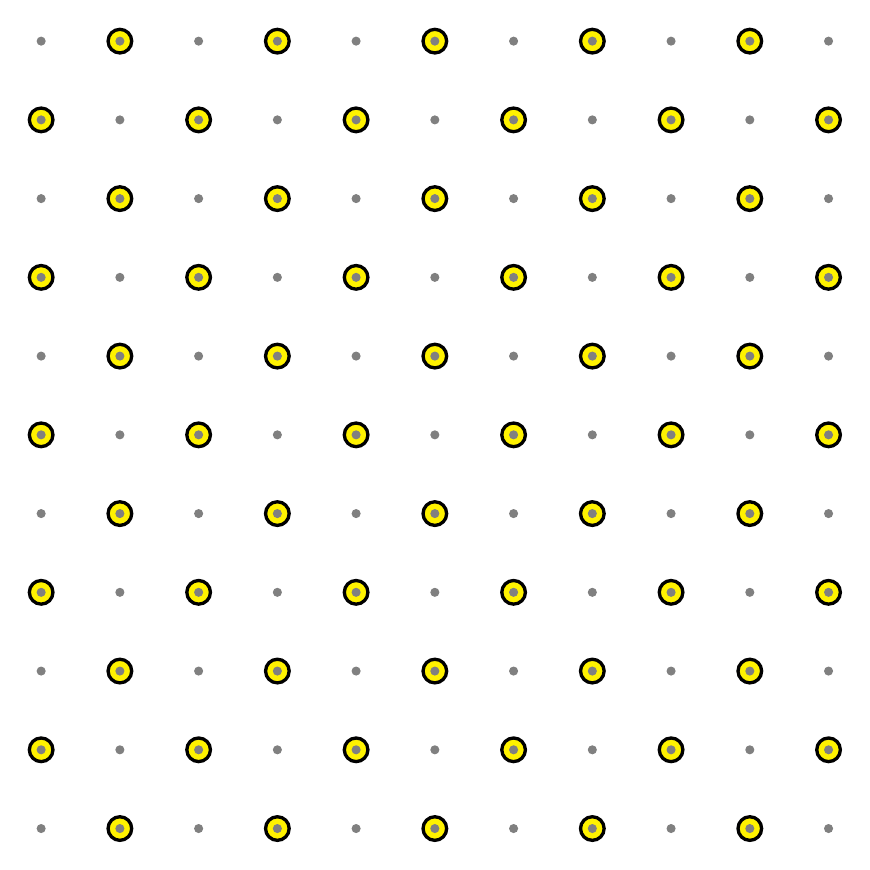
\begin{tikzpicture}
\foreach \x in {0,...,10}{
	\foreach \y in {0,...,10}{
	\ADD{\x}{\y}{\z}
	\ifodd\z
		\draw (\x,\y)node[bigdot]{};
	\fi
	\draw (\x,\y)node[smalldot]{};

		}}

\end{tikzpicture}
\caption{Blank Starting Grid}\label{fig:start}
\end{figure}

If we have a totally blank knot -- basically just a weave-- the strands will travel diagonally across the grid, crossing at the highlighted dots (Figure~\ref{fig:blank}).

\begin{figure}[H]
\centering
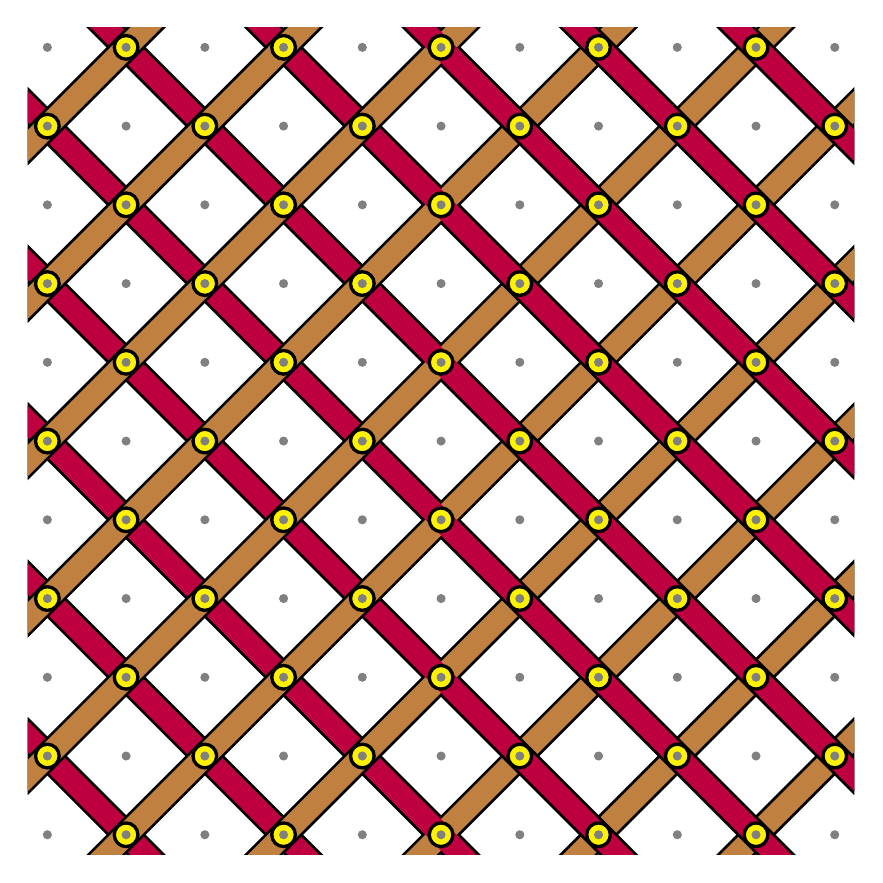
\begin{tikzpicture}
\begin{scope}
\clip (-.25,-.25) rectangle (10.25,10.25);
\foreach \y in {-9,-7,...,9}{
\draw[line width=10pt] (-.5,\y-.5)--(10.5,10.5+\y) (-.5,10.5+\y)--(10.5,\y-.5);
\draw[brown,line width=8pt](-.5,\y-.5)--(10.5,10.5+\y);
\draw[purple,line width=8pt] (-.5,10.5+\y)--(10.5,\y-.5);
}
\end{scope}

\foreach \x in {0,...,10}{
	\foreach \y in {0,...,10}{
	\ADD{\x}{\y}{\z}
	\ifodd\z
		\draw (\x,\y)node[bigdot]{};
	\fi
	\draw (\x,\y)node[smalldot]{};
		}}

\end{tikzpicture}
\caption{Blank Knot}\label{fig:blank}
\end{figure}

To add features to the knot, draw vertical or horizontal lines at the highlighted dots, stretching from one background dot to another. At these lines, the usual crossing is broken, and replaced with two curves.

If you're drawing these by hand, the following mental image might be useful. At every dot, the strand would like to travel to the next dot diagonally. When it hits one of these lines, that's a wall, deflecting its path.
\begin{figure}[H]
\centering
\begin{subfigure}[t]{.3\textwidth}
		\centering
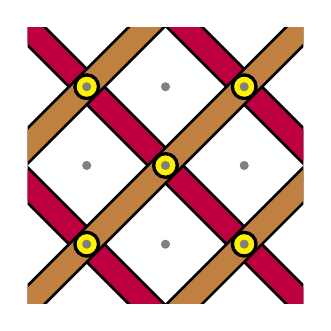
\begin{tikzpicture}
\clip (.25,1.25) rectangle (3.75,4.75);
\foreach \y in {-7,-5,-3,-1,1,3}{
\draw[line width=10pt] (-.5,\y-.5)--(10.5,10.5+\y) (-.5,10.5+\y)--(10.5,\y-.5);
\draw[brown,line width=8pt](-.5,\y-.5)--(10.5,10.5+\y);
\draw[purple,line width=8pt] (-.5,10.5+\y)--(10.5,\y-.5);
}

\foreach \x in {0,...,4}{
	\foreach \y in {0,...,4}{
	\ADD{\x}{\y}{\z}
	\ifodd\z
		\draw (\x,\y)node[bigdot]{};
	\fi
	\draw (\x,\y)node[smalldot]{};
		}}
\end{tikzpicture}
		\caption{Centre dot unmarked}
	\end{subfigure}
\hfill
	\begin{subfigure}[t]{.3\textwidth}
		\centering
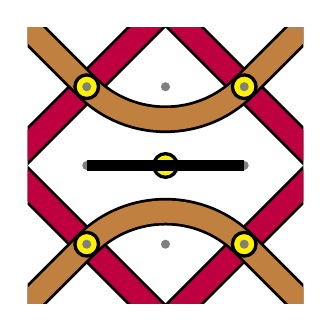
\begin{tikzpicture}[rotate=90]
\clip (.25,1.25) rectangle (3.75,4.75);

\draw[line width=10pt](2,1)--(4,3)--(2,5)--(0,3)--cycle;
\draw[purple,line width=8pt](2,1)--(4,3)--(2,5)--(0,3)--cycle;
\draw[line width=10pt](0,1)-- (1,2) to[bend right=45] (1,4)--(0,5);
\draw[brown,line width=8pt](0,1)-- (1,2) to[bend right=45] (1,4)--(0,5);
\draw[line width=10pt](4,1)--(3,2) to[bend left=45] (3,4)--(4,5);
\draw[brown,line width=8pt](4,1)--(3,2) to[bend left=45] (3,4)--(4,5);
\foreach \x in {0,...,4}{
	\foreach \y in {0,...,4}{
	\ADD{\x}{\y}{\z}
	\ifodd\z
		\draw (\x,\y)node[bigdot]{};
	\fi
	\draw (\x,\y)node[smalldot]{};
		}}
\draw[line width=4pt] (2,2)--(2,4);
\end{tikzpicture}
		\caption{Centre dot with horizontal line}\label{sfig:quarterturn}
	\end{subfigure}
%
\hfill
	\begin{subfigure}[t]{.3\textwidth}
		\centering
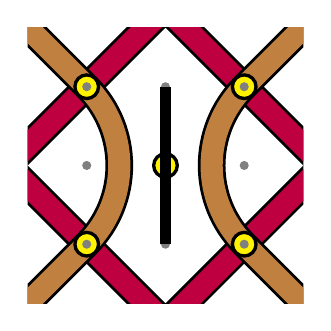
\begin{tikzpicture}
\clip (.25,1.25) rectangle (3.75,4.75);

\draw[line width=10pt](2,1)--(4,3)--(2,5)--(0,3)--cycle;
\draw[purple,line width=8pt](2,1)--(4,3)--(2,5)--(0,3)--cycle;
\draw[line width=10pt](0,1)-- (1,2) to[bend right=45] (1,4)--(0,5);
\draw[brown,line width=8pt](0,1)-- (1,2) to[bend right=45] (1,4)--(0,5);
\draw[line width=10pt](4,1)--(3,2) to[bend left=45] (3,4)--(4,5);
\draw[brown,line width=8pt](4,1)--(3,2) to[bend left=45] (3,4)--(4,5);
\foreach \x in {0,...,4}{
	\foreach \y in {0,...,4}{
	\ADD{\x}{\y}{\z}
	\ifodd\z
		\draw (\x,\y)node[bigdot]{};
	\fi
	\draw (\x,\y)node[smalldot]{};
		}}
\draw[line width=4pt] (2,2)--(2,4);
\end{tikzpicture}
		\caption{Centre dot with vertical line}
	\end{subfigure}

\caption{Single feature wall}
\end{figure}
We want our knot to not wander off the picture, so let's add these feature walls around the border of the blank knot. We come into a new situation at the corners: two feature walls that touch each other. Feature walls should never \textit{cross} one another, but they might meet at their ends. When this happens, we keep our mental image of the feature walls as walls that deflect the knot strands. This causes our strands to make a corner.

\begin{figure}[H]
\centering
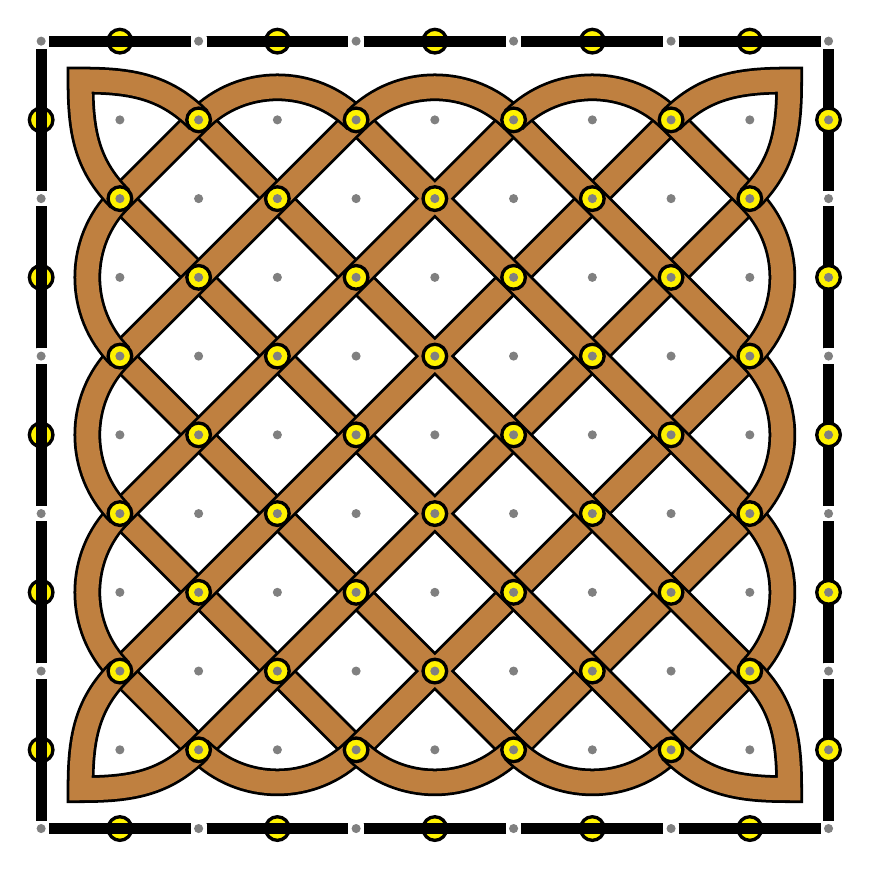
\begin{tikzpicture}
\begin{scope}
\clip (1,1) rectangle (9,9);
\foreach \y in {-9,-7,...,9}{
\draw[line width=10pt] (-.5,\y-.5)--(10.5,10.5+\y) (-.5,10.5+\y)--(10.5,\y-.5);
\draw[brown,line width=8pt](-.5,\y-.5)--(10.5,10.5+\y);
\draw[brown,line width=8pt] (-.5,10.5+\y)--(10.5,\y-.5);
}
\end{scope}

\foreach \x in {3,5,7}{
\draw[line width=10pt] (\x-1,1) to[bend right=45] (\x+1,1)(1,\x-1) to[bend left=45] (1,\x+1)(\x-1,9) to[bend left=45] (\x+1,9)(9,\x-1) to[bend right=45] (9,\x+1);
\draw[brown,line width=8pt] (\x-1,1) to[bend right=45] (\x+1,1)(1,\x-1) to[bend left=45] (1,\x+1)(\x-1,9) to[bend left=45] (\x+1,9)(9,\x-1) to[bend right=45] (9,\x+1);
}

\draw[line width=10pt] (8,9) to[out=45, in=180](9.5,9.5) to[out=270,in=45](9,8);
\draw[line width=10pt] (1,2) to[out=225, in=90](.5,.5) to[out=0,in=225](2,1);
\draw[line width=10pt] (1,8) to[out=135, in=270](.5,9.5) to[out=00,in=135](2,9);
\draw[line width=10pt] (8,1) to[out=-45, in=180](9.5,.5) to[out=90,in=-45](9,2);
\draw[brown,line width=8pt] (8,9) to[out=45, in=180](9.5,9.5) to[out=270,in=45](9,8);
\draw[brown,line width=8pt] (1,2) to[out=225, in=90](.5,.5) to[out=0,in=225](2,1);
\draw[brown,line width=8pt] (1,8) to[out=135, in=270](.5,9.5) to[out=00,in=135](2,9);
\draw[brown,line width=8pt] (8,1) to[out=-45, in=180](9.5,.5) to[out=90,in=-45](9,2);

\foreach \x in {0,...,10}{
	\foreach \y in {0,...,10}{
	\ADD{\x}{\y}{\z}
	\ifodd\z
		\draw (\x,\y)node[bigdot]{};
	\fi
	\draw (\x,\y)node[smalldot]{};
	\ifodd\x
		\draw[line width=4pt] (\x-.9,0)--(\x+.9,0) (\x-.9,10)--(\x+.9,10) 
		 (0,\x-.9)--(0,\x+.9) (10,\x-.9)--(10,\x+.9) ;		 
	\fi
		}}

\end{tikzpicture}
\caption{Blank Knot with Borders}
\end{figure}

From here, experiment with adding feature walls on the interior highlighted dots. Where two lines meet at a corner, the strand makes a corner. For aesthetic reasons, I like to draw it with a point, rather than as a smooth curve.

It's possible also to have three feature walls make a dead end. This makes a self-twist in the strand.

\begin{figure}[H]
\centering
\begin{subfigure}[t]{.3\textwidth}
		\centering
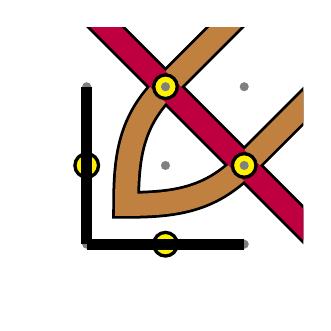
\begin{tikzpicture}
\clip (2.25,2.25) rectangle (5.75,5.75);

\draw[line width=10pt] (5,6)--(4,5) to[out=225,in=90] (3.5,3.5) to[out=0, in=225](5,4)--(6,5);
\draw[line width=10pt] (3,6)--(6,3);
\draw[line width=8pt,brown] (5,6)--(4,5) to[out=225,in=90] (3.5,3.5) to[out=0, in=225](5,4)--(6,5);
\draw[line width=8pt,purple] (3,6)--(6,3);


\foreach \x in {0,...,8}{
	\foreach \y in {0,...,8}{
	\ADD{\x}{\y}{\z}
	\ifodd\z
		\draw (\x,\y)node[bigdot]{};
	\fi
	\draw (\x,\y)node[smalldot]{};
		}}
\draw[line width=4pt] (3,3)--(5,3) (3,3)--(3,5);
\end{tikzpicture}
		\caption{Corner Point}\label{sfig:cornerpoint}
	\end{subfigure}
\hfill
	\begin{subfigure}[t]{.3\textwidth}
		\centering
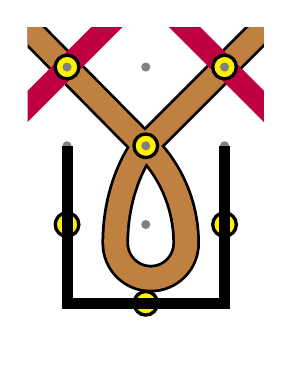
\begin{tikzpicture}
\clip (.5,.25) rectangle (3.5,4.5);
\draw[line width=10pt] (4,5)--(2,3)
 arc(45:0:1.75cm and 1.75 cm) arc (0:-180:4.5mm) arc (180:135:1.25 cm and 1.75 cm)
% arc(45:0:1cm and 1.5 cm) arc (0:-180:3mm) arc (180:135:1 cm and 1.5 cm)%to[out=225,in=90](1.5,1.5)--(2.5,1.5)to[out=90,in=-45](2,3)
--(0,5);
\draw[line width=8pt,brown] (4,5)--(2,3)
 arc(45:0:1.75cm and 1.75 cm) arc (0:-180:4.5mm) arc (180:135:1.25 cm and 1.75 cm)
% arc(45:0:1cm and 1.5 cm) arc (0:-180:3mm) arc (180:135:1 cm and 1.5 cm)
%to[out=225,in=90](1.5,1.5)--(2.5,1.5)to[out=90,in=-45](2,3)
--(0,5);
\draw[line width=8pt,purple] (0,3)--(2,5)--(4,3);

\foreach \x in {0,...,8}{
	\foreach \y in {0,...,8}{
	\ADD{\x}{\y}{\z}
	\ifodd\z
		\draw (\x,\y)node[bigdot]{};
	\fi
	\draw (\x,\y)node[smalldot]{};
		}}
\draw[line width=4pt] (1,3)--(1,1)--(3,1)--(3,3);
\end{tikzpicture}
		\caption{Twist}\label{sfig:twist}
	\end{subfigure}
%
\hfill
	\begin{subfigure}[t]{.3\textwidth}
		\centering
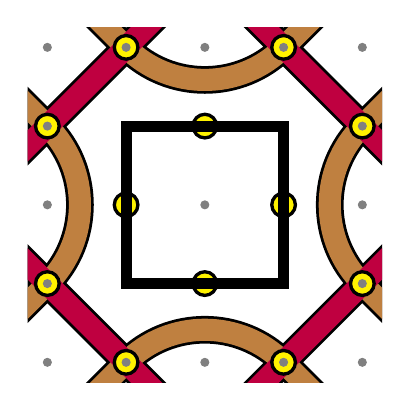
\begin{tikzpicture}
\clip (1.75,1.75) rectangle (6.25,6.25);

\draw[line width=10pt] (2,1)--(3,2)to[bend left=45](5,2)--(6,1)
 (7,2)--(6,3)to[bend left=45](6,5)--(7,6)
 (6,7)-- (5,6)to[bend left=45](3,6)--(2,7)
 (1,6)--  (2,5)to[bend left=45](2,3)--(1,2)
   (4,1)--(7,4)--(4,7)--(1,4)--cycle;
\draw[line width=8pt,brown] (2,1)--(3,2)to[bend left=45](5,2)--(6,1)
 (7,2)--(6,3)to[bend left=45](6,5)--(7,6)
 (6,7)-- (5,6)to[bend left=45](3,6)--(2,7)
 (1,6)--  (2,5)to[bend left=45](2,3)--(1,2);
\draw[line width=8pt,purple]    (4,1)--(7,4)--(4,7)--(1,4)--cycle;

\foreach \x in {0,...,8}{
	\foreach \y in {0,...,8}{
	\ADD{\x}{\y}{\z}
	\ifodd\z
		\draw (\x,\y)node[bigdot]{};
	\fi
	\draw (\x,\y)node[smalldot]{};
		}}
\draw[line width=4pt] (3,3)rectangle (5,5);
\end{tikzpicture}

		\caption{Hole}
	\end{subfigure}

\caption{Combinations of feature walls}
\end{figure}


If you add adjacent rows of parallel feature walls, you'll get a run -- a long straight horizontal or vertical piece. This case is significantly more complicated than the others, so we've included it at the end of this chapter, in \ref{ssec:drawruns}


%%%%%%%%%%%%
%%%%%%%%%%%%

When your feature walls are all added, now you can add in the crossings. At every crossing, one strand will go on top, and the other on the bottom. The hard way of doing this is following a strand, and keeping track of over/under for yourself. The easy way is to recognize that all crossings in a row or column have the same crossing orientation: in all of them, the top strand has the same orientation (bottom left to top right, or bottom right to top left). 

The knot in Figure~\ref{fig:crossinglines} has no internal feature walls, but even with feature walls, each row or column will have the same crossing orientations.


\begin{figure}[H]
\centering
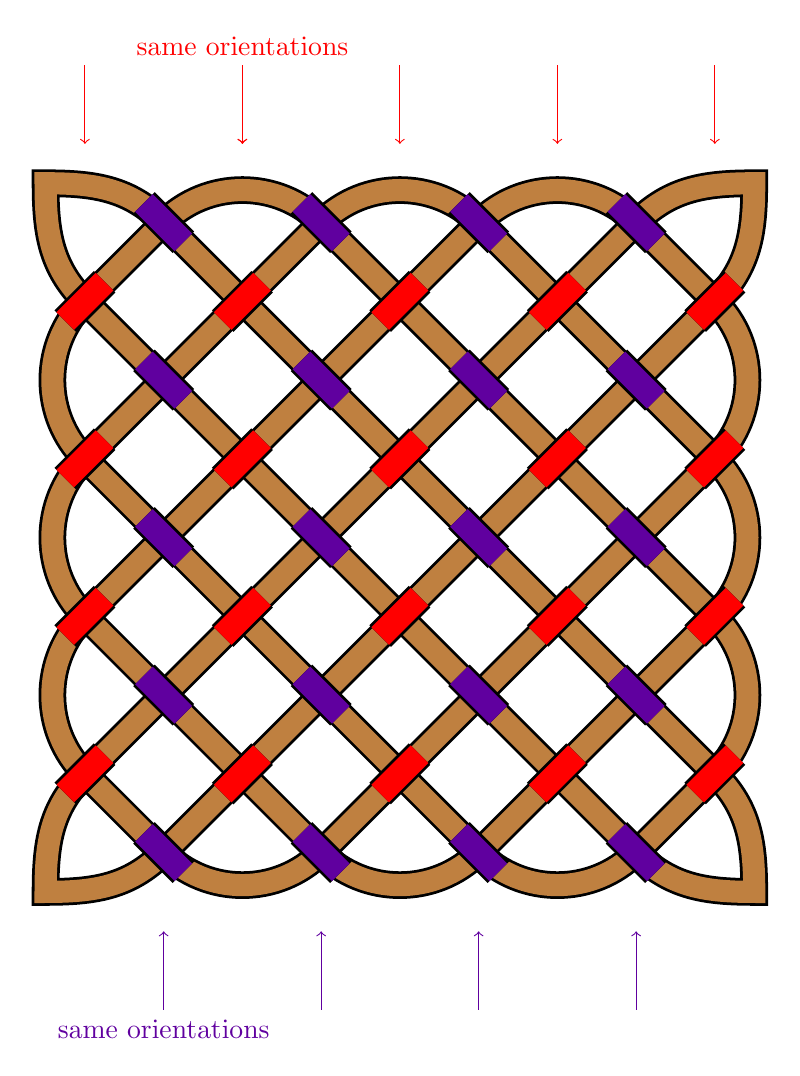
\begin{tikzpicture}
\begin{scope}
\clip (1,1) rectangle (9,9);
\foreach \y in {-9,-7,...,9}{
\draw[line width=10pt] (-.5,\y-.5)--(10.5,10.5+\y) (-.5,10.5+\y)--(10.5,\y-.5);
\draw[brown,line width=8pt](-.5,\y-.5)--(10.5,10.5+\y);
\draw[brown,line width=8pt] (-.5,10.5+\y)--(10.5,\y-.5);
}
\end{scope}

\foreach \x in {3,5,7}{
\draw[line width=10pt] (\x-1,1) to[bend right=45] (\x+1,1)
(1,\x-1) to[bend left=45] (1,\x+1)
(\x-1,9) to[bend left=45] (\x+1,9)
(9,\x-1) to[bend right=45] (9,\x+1)
;
\draw[brown,line width=8pt] (\x-1,1) to[bend right=45] (\x+1,1)
(1,\x-1) to[bend left=45] (1,\x+1)
(\x-1,9) to[bend left=45] (\x+1,9)
(9,\x-1) to[bend right=45] (9,\x+1)
;
	}
	
\draw[line width=10pt] (8,9) to[out=45, in=180](9.5,9.5) to[out=270,in=45](9,8);
\draw[line width=10pt] (1,2) to[out=225, in=90](.5,.5) to[out=0,in=225](2,1);
\draw[line width=10pt] (1,8) to[out=135, in=270](.5,9.5) to[out=00,in=135](2,9);
\draw[line width=10pt] (8,1) to[out=-45, in=180](9.5,.5) to[out=90,in=-45](9,2);

\draw[brown,line width=8pt] (8,9) to[out=45, in=180](9.5,9.5) to[out=270,in=45](9,8);
\draw[brown,line width=8pt] (1,2) to[out=225, in=90](.5,.5) to[out=0,in=225](2,1);
\draw[brown,line width=8pt] (1,8) to[out=135, in=270](.5,9.5) to[out=00,in=135](2,9);
\draw[brown,line width=8pt] (8,1) to[out=-45, in=180](9.5,.5) to[out=90,in=-45](9,2);

\foreach \x in {1,...,9}{
	\foreach \y in {1,...,9}{
		\ifodd\x
			\ifodd\y
			\else
			\draw[line width=11pt] (\x-.25,\y-.25)--(\x+.25,\y+.25);
			\draw[line width=9pt,red] (\x-.25,\y-.25)--(\x+.25,\y+.25);
			\fi
		\else
			\ifodd\y
			\draw[line width=11pt] (\x-.25,\y+.25)--(\x+.25,\y-.25);
			\draw[line width=9pt,blue!50!purple] (\x-.25,\y+.25)--(\x+.25,\y-.25);
			\fi
		\fi
		
		}}
\draw[<-,purple!50!blue] (2,0)--(2,-1)node[below]{same orientations};
\draw[<-,red] (3,10)--(3,11)node[above]{same orientations};
\foreach \x in {4,6,8}{\draw[<-,purple!50!blue](\x,0)--(\x,-1);}
\foreach \x in {1,3,5,7,9}{\draw[<-,red](\x,10)--(\x,11);}
\end{tikzpicture}
\caption{Knot with Crossings}\label{fig:crossinglines}
\end{figure}

Although this method requires the grid to be rectilinear (i.e. made out of horizontal and vertical lines), it doesn't have to actually be a rectangle. You can block out different shapes from an underlying rectangular grid. For example, in a large enough piece, you could approximate a circular outline.

\begin{figure}[H]
\centering
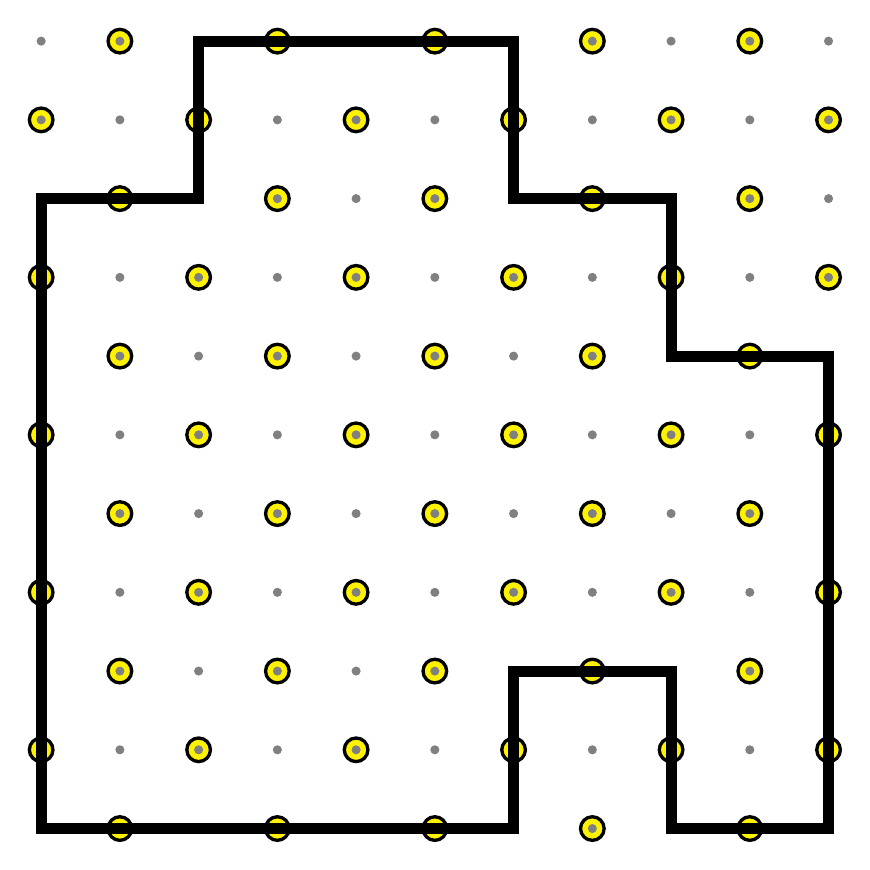
\begin{tikzpicture}
\foreach \x in {0,...,10}{
	\foreach \y in {0,...,10}{
	\ADD{\x}{\y}{\z}
	\ifodd\z
		\draw (\x,\y)node[bigdot]{};
	\fi
	\draw (\x,\y)node[smalldot]{};
		}}
\draw[line width=4pt](4,0)--(6,0)--(6,2)--(8,2)--(8,0)--(10,0)--(10,6)--(8,6)--(8,8)--(6,8)--(6,10)--(2,10)--(2,8)--(0,8)--(0,0)--cycle;
\end{tikzpicture}
\caption{Alternate Grid Shape}\label{fig:rectilinear}
\end{figure}
%%%%%%%%%%%%%%%%%%%%%%%%%%%%%%%%

\section{Practical Considerations}
For knots that you will turn into physical objects, the end use of the object should be taken into consideration. For example, anything that won't spend its life laying down, or tacked to something else, probably shouldn't have any large continuous gaps. So you might want to stay away from long strings of feature walls that make big slits in the pattern.

Similarly, a twist caused by three feature walls making a dead end (see Figure~\ref{sfig:twist}) will lead to a flappy bit. This is probably also best reserved for pieces that will lay flat.

Something else to consider in your finished pattern is how many separate strands make it up. This is harder to determine, since there's no easy local test for it (like looking at feature walls in a small area). Follow the strand around, possibly colouring it, until you loop back on yourself. Longer strands are somewhat harder to arrange when it comes time to assemble your piece. Not impossible, surely, but keep in mind you'll want to be extra careful labelling your intersections (more in Chapter~\ref{sec:making}). If you do want to use a pattern with a very long strand, consider breaking the strand into several pieces and sewing them together.

%%%%%%%%%%%%%%

\section{Special Case: Drawing Runs}\label{ssec:drawruns}
When you add parallel adjacent feature walls, the strand turns into a vertical or horizontal straight line, called a run. That part is easy enough to draw. The hard part comes when the run ends. The easiest way to draw these is to keep in mind the ``deflecting" paradigm, that strands want to go to their diagonally-adjacent dot, but are deflected when they run into a feature wall. The exposition below goes into greater detail about the various cases, but if you're comfortable drawing using the deflection model, you shouldn't need this level of detail for knot drawing. (You \emph{will} need this level of detail for translating a knot that contains a run into a crochet pattern.)

In the simplest case, the run ends directly at a crossing. That is, the strand goes from the run directly to a dot. For this case, draw a smooth arc from the end of the run to the dot. The strand should make a 45-degree turn, so it's back in its usual diagonal orientation when it hits the dot.

\begin{figure}[H]
\begin{subfigure}[t]{.49\textwidth}
		\centering
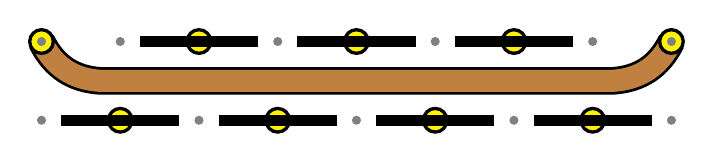
\begin{tikzpicture}
\draw[line width=10pt] (0,1)to[bend right](.75,.5)--(7.25,.5)to[bend right](8,1);
\draw[line width=8pt,brown] (0,1)to[bend right](.75,.5)--(7.25,.5)to[bend right](8,1);

\foreach \x in {0,...,8}{
	\foreach \y in {0,1}{
	\ADD{\x}{\y}{\z}
	\ifodd\z
		\draw (\x,\y)node[bigdot]{};
	\fi
	\draw (\x,\y)node[smalldot]{};
		}}
\foreach \x in {1,3,5,7}{
	\draw[line width=4pt] (\x-0.75,0)--(\x+.75,0);}
\foreach \x in {2,4,6}{
	\draw[line width=4pt] (\x-0.75,1)--(\x+.75,1);}
\end{tikzpicture}
\caption{Run using an odd number of feature walls (seven)}
\end{subfigure}
\qquad
\begin{subfigure}[t]{.49\textwidth}
		\centering
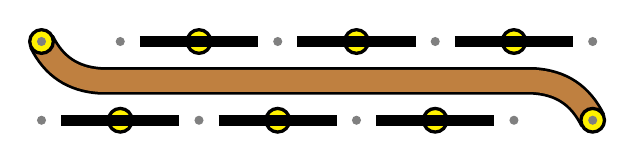
\begin{tikzpicture}
\draw[line width=10pt](0,1)to[bend right](.75,.5)--(6.25,.5)to[bend left](7,0);
\draw[line width=8pt,brown] (0,1)to[bend right](.75,.5)--(6.25,.5)to[bend left](7,0);

\foreach \x in {0,...,7}{
	\foreach \y in {0,1}{
	\ADD{\x}{\y}{\z}
	\ifodd\z
		\draw (\x,\y)node[bigdot]{};
	\fi
	\draw (\x,\y)node[smalldot]{};
		}}
\foreach \x in {1,3,5}{
	\draw[line width=4pt] (\x-0.75,0)--(\x+.75,0);}
\foreach \x in {2,4,6}{
	\draw[line width=4pt] (\x-0.75,1)--(\x+.75,1);}
\end{tikzpicture}
\caption{Run using an even number of feature walls (six)}
\end{subfigure}
\caption{D-type corners}\label{fig:featurerun}
\end{figure}

We call this type of corner D-type, where D stands for ``direct." If the first dot after a run has
a feature wall, then the corner will be of a different type.

\medskip
 %If its feature wall is parallel to the run, then that dot is actually still part of the run, extending the existing walls. So that feature wall must be \textit{perpendicular} to the run.


%%%%%%%%%%%%
\begin{figure}[H]
\begin{subfigure}[t]{.49\textwidth}
		\centering
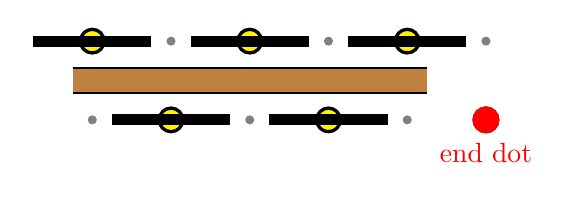
\begin{tikzpicture}
\draw[line width=10pt] (1.75,.5)--(6.25,.5);
\draw[line width=8pt,brown](1.75,.5)--(6.25,.5);

\foreach \x in {2,...,7}{
	\foreach \y in {0,1}{
	\ADD{\x}{\y}{\z}
	\ifodd\z
		\draw (\x,\y)node[bigdot]{};
	\fi
	\draw (\x,\y)node[smalldot]{};
		}}
\draw[red] (7,0)node[bigdot,red,label=below:{end dot}]{};
\foreach \x in {3,5}{
	\draw[line width=4pt] (\x-0.75,0)--(\x+.75,0);}
\foreach \x in {2,4,6}{
	\draw[line width=4pt] (\x-0.75,1)--(\x+.75,1);}
\end{tikzpicture}
\caption{End dot has no wall: D-type(see Figure~\ref{fig:featurerun})}
\end{subfigure}
\hspace{1cm}
\begin{subfigure}[t]{.49\textwidth}
		\centering
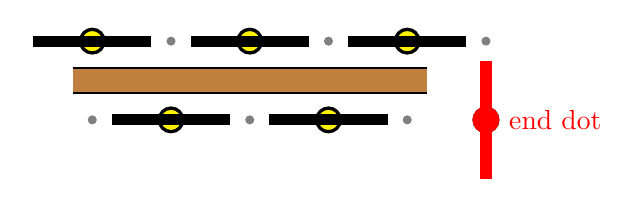
\begin{tikzpicture}
\draw[line width=10pt] (1.75,.5)--(6.25,.5);
\draw[line width=8pt,brown](1.75,.5)--(6.25,.5);

\foreach \x in {2,...,7}{
	\foreach \y in {0,1}{
	\ADD{\x}{\y}{\z}
	\ifodd\z
		\draw (\x,\y)node[bigdot]{};
	\fi
	\draw (\x,\y)node[smalldot]{};
		}}
\draw[red] (7,0)node[bigdot,red,label=right:{end dot}]{};
\foreach \x in {3,5}{
	\draw[line width=4pt] (\x-0.75,0)--(\x+.75,0);}
\foreach \x in {2,4,6}{
	\draw[line width=4pt] (\x-0.75,1)--(\x+.75,1);}
\draw[red,line width=4pt] (7,.75)--(7,-.75);%node[below]{end dot};
\end{tikzpicture}
\caption{End dot has perpendicular wall: not D-type}\label{sfig:perpwallgroup}
\end{subfigure}
\qquad
\caption{End of a Run}\label{fig:endrun}
\end{figure}
%%%%%%%%%%%%
If the red dots in Figure~\ref{fig:endrun} had a horizontal feature wall, they would just be a part of the run. So the end dot of a run will not have a feature wall parallel to the run.  So, they can either have no feature wall (and be a D-type corner, as in Figure~\ref{fig:featurerun}), or a feature wall perpendicular to the direction of the run (in the cases pictures above, vertical). This perpendicular feature wall will cause the strand to bend. Now, we consider the next dot the strand would be heading towards.



In the situation shown in Figure~\ref{sfig:perpwallgroup}, the strand will be ``deflected" downwards by the red wall. In this case, we turn our attention to the \textcolor{green}{next dot} the strand wants to go to, shown in green below.
\begin{figure}[H]\centering
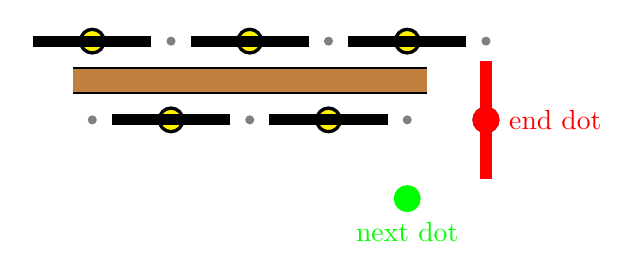
\begin{tikzpicture}
\draw[line width=10pt] (1.75,.5)--(6.25,.5);
\draw[line width=8pt,brown](1.75,.5)--(6.25,.5);

\foreach \x in {2,...,7}{
	\foreach \y in {0,1}{
	\ADD{\x}{\y}{\z}
	\ifodd\z
		\draw (\x,\y)node[bigdot]{};
	\fi
	\draw (\x,\y)node[smalldot]{};
		}}
\draw[red] (7,0)node[bigdot,red,label=right:{end dot}]{};
\foreach \x in {3,5}{
	\draw[line width=4pt] (\x-0.75,0)--(\x+.75,0);}
\foreach \x in {2,4,6}{
	\draw[line width=4pt] (\x-0.75,1)--(\x+.75,1);}
\draw[red,line width=4pt] (7,.75)--(7,-.75);%node[below]{end dot};
\draw[green] (6,-1)node[bigdot,green,label=below:{next dot}]{};
\end{tikzpicture}

\caption{Next dot at the end of a run}\label{fig:nextdotrun}
\end{figure}

The green dot can have no wall, a wall parallel to the run, or a wall perpendicular to the run.


%%%%%%%%%%%%
\begin{figure}[H]
\begin{subfigure}[t]{.3\textwidth}
		\centering
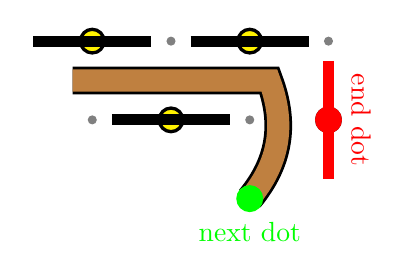
\begin{tikzpicture}
\draw[line width=10pt] (3.75,.5)--(6.25,.5)to[bend left](6,-1);
\draw[line width=8pt,brown](3.75,.5)--(6.25,.5)to[bend left](6,-1);

\foreach \x in {4,...,7}{
	\foreach \y in {0,1}{
	\ADD{\x}{\y}{\z}
	\ifodd\z
		\draw (\x,\y)node[bigdot]{};
	\fi
	\draw (\x,\y)node[smalldot]{};
		}}
\draw[red] (7,0)node[bigdot,red,label=right:{\rotatebox{-90}{end dot}}]{};
\foreach \x in {5}{
	\draw[line width=4pt] (\x-0.75,0)--(\x+.75,0);}
\foreach \x in {4,6}{
	\draw[line width=4pt] (\x-0.75,1)--(\x+.75,1);}
\draw[red,line width=4pt] (7,.75)--(7,-.75);%node[below]{end dot};
\draw[green] (6,-1)node[bigdot,green,label=below:{next dot}]{};
\end{tikzpicture}
\caption{\textcolor{green}{next dot} has no feature wall: J-type}\label{sfig:nextclear}
\end{subfigure}
\quad
%%%%
\begin{subfigure}[t]{.3\textwidth}
		\centering
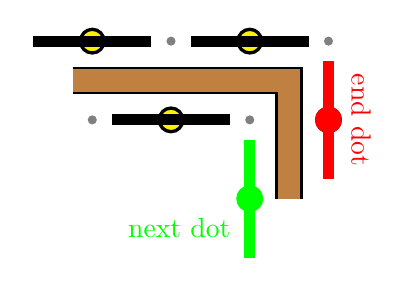
\begin{tikzpicture}
\draw[line width=10pt] (3.75,.5)-|(6.5,-1);
\draw[line width=8pt,brown](3.75,.5)-|(6.5,-1);

\foreach \x in {4,...,7}{
	\foreach \y in {0,1}{
	\ADD{\x}{\y}{\z}
	\ifodd\z
		\draw (\x,\y)node[bigdot]{};
	\fi
	\draw (\x,\y)node[smalldot]{};
		}}
\draw[red] (7,0)node[bigdot,red,label=right:{\rotatebox{-90}{end dot}}]{};
\foreach \x in {5}{
	\draw[line width=4pt] (\x-0.75,0)--(\x+.75,0);}
\foreach \x in {4,6}{
	\draw[line width=4pt] (\x-0.75,1)--(\x+.75,1);}
\draw[red,line width=4pt] (7,.75)--(7,-.75);%node[below]{end dot};
\draw[green] (6,-1)node[bigdot,green,label=below left:{next dot}]{};
\draw[green,line width=4pt] (6,-1.75)--(6.,-.25);
\end{tikzpicture}
\caption{\textcolor{green}{next dot} has perpendicular feature wall: L-type}\label{sfig:nextcorner}
\end{subfigure}
\quad
%%%%
\begin{subfigure}[t]{.3\textwidth}
		\centering
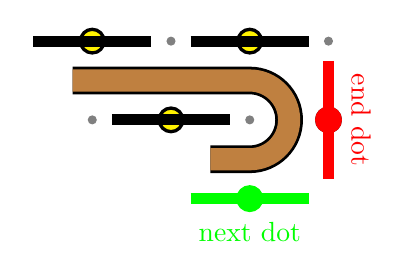
\begin{tikzpicture}
\draw[line width=10pt] (3.75,.5)--(6.,.5)arc(90:-90:5mm)--+(-.5,0);
\draw[line width=8pt,brown](3.75,.5)--(6.,.5)arc(90:-90:5mm)--+(-.5,0);

\foreach \x in {4,...,7}{
	\foreach \y in {0,1}{
	\ADD{\x}{\y}{\z}
	\ifodd\z
		\draw (\x,\y)node[bigdot]{};
	\fi
	\draw (\x,\y)node[smalldot]{};
		}}
\draw[red] (7,0)node[bigdot,red,label=right:{\rotatebox{-90}{end dot}}]{};
\foreach \x in {5}{
	\draw[line width=4pt] (\x-0.75,0)--(\x+.75,0);}
\foreach \x in {4,6}{
	\draw[line width=4pt] (\x-0.75,1)--(\x+.75,1);}
\draw[red,line width=4pt] (7,.75)--(7,-.75);%node[below]{end dot};
\draw[green] (6,-1)node[bigdot,green,label=below:{next dot}]{};
\draw[green,line width=4pt] (5.25,-1)--(6.75,-1);
\end{tikzpicture}
\caption{\textcolor{green}{next dot} has parallel feature wall: C-type}\label{sfig:nextrun}
\end{subfigure}
\caption{J-type, L-type, and C-type corners}\label{fig:nextrun}
\end{figure}

If the \textcolor{green}{next dot} has no feature wall (Figure~\ref{sfig:nextclear}), make a  corner at ``end dot," then a smooth arc from the run to the green dot.  You are now at a crossing, and the component has ended.  Since the strand makes a turn that looks like the letter J, we call this a J-type corner.

If the \textcolor{green}{next dot} has a feature wall perpendicular to the original run (parallel to the wall on the end dot, as shown in  Figure~\ref{sfig:nextcorner}), then the strand makes a right-angle turn. It is now starting a new run, perpendicular to the last. There has been no crossing, so you are still in the same component. Since the strand makes an L-shape, we call this an L-type corner.

If the \textcolor{green}{next dot} has a feature wall parallel to the original run (perpendicular to the wall on the end dot, as shown in  Figure~\ref{sfig:nextrun}), the strand makes a half-circle. It is now starting a new run, parallel to the last.  There has been no crossing, so you are still in the same component. Since the strand makes a C-shape turn, we call this a C-type corner.
%%%%%%%%%%
%%%%%%%%%%%%

%%%%%%%%%%%%
\begin{figure}[h]
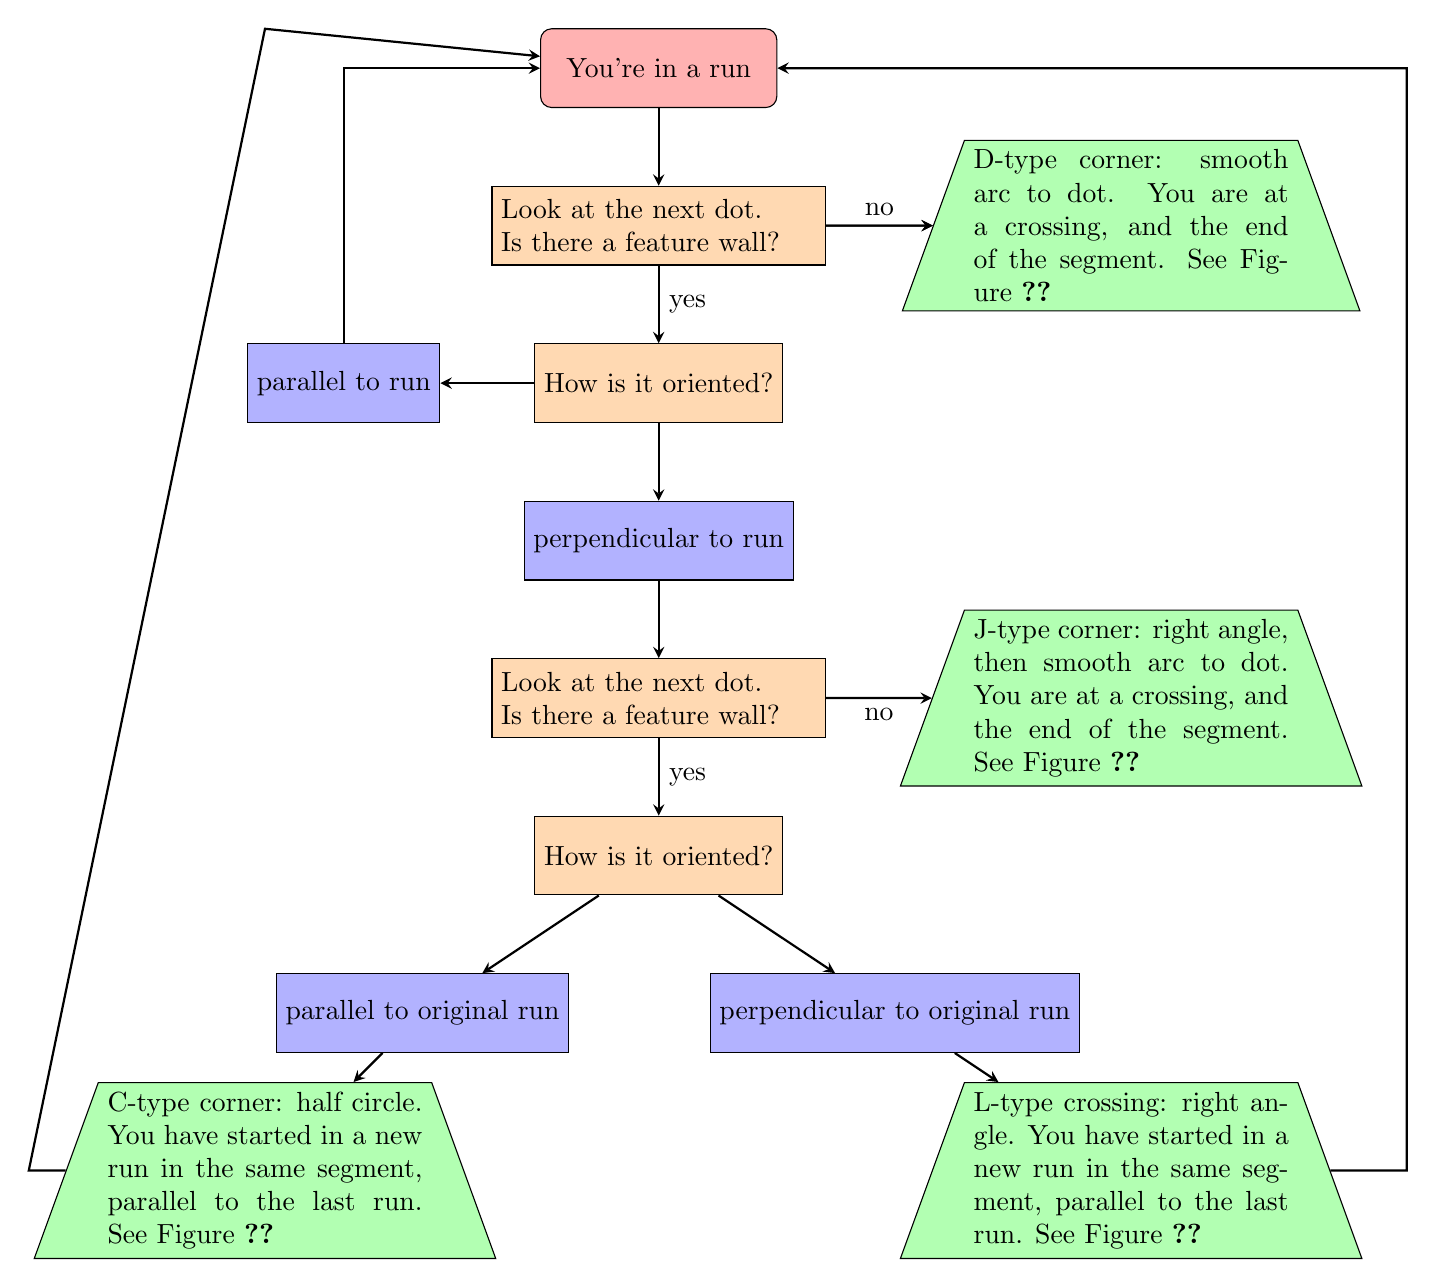
\begin{tikzpicture}[node distance=2cm]
\node (start) [startstop] {You're in a run};

\node (FW1) [process, below of=start] {\parbox{4cm}{Look at the next dot.\\ Is there a feature wall?}};
\draw [arrow] (start)--(FW1);


\node (WYN2) [decision,right of=FW1,xshift=4cm]{\parbox{4cm}{D-type corner: smooth arc to dot. You are at a crossing, and the end of the segment. See Figure~\ref{fig:featurerun}}};
\draw [arrow] (FW1)--node[anchor=south]{no}(WYN2);
\draw [arrow] (FW1)--(WYN2);


\node (or1) [process,below of =FW1] {How is it oriented?};
\draw [arrow] (FW1)--node[anchor=west]{yes}(or1);

\node (end2) [io, left of=or1,xshift=-2cm]  {parallel to run};
\node (end1) [io, below of=or1] {perpendicular to run};
\draw[arrow] (or1) -- (end1);
\draw[arrow] (or1) -- (end2);
\draw[arrow] (end2)|-(start);

\node (FW2) [process, below of=end1] {\parbox{4cm}{Look at the next dot.\\ Is there a feature wall?}};

\node(WYN3) [decision,right of=FW2,xshift=4cm]{\parbox{4cm}{J-type corner: right angle, then smooth arc to dot. You are at a crossing, and the end of the segment. See
Figure~\ref{sfig:nextclear}}};

\draw[arrow](end1)--(FW2);
\draw [arrow] (FW2)-- node[anchor=north]{no}(WYN3);

\node (or2) [process,below of =FW2] {How is it oriented?};
\draw [arrow] (FW2)--node[anchor=west]{yes}(or2);

\node (parallel2) [io,below of = or2, xshift=-3cm] {parallel to original run};
\node (perpendicular2) [io,below of = or2, xshift=3cm] {perpendicular to original run};
\draw [arrow] (or2)--(parallel2);
\draw [arrow] (or2)--(perpendicular2);

\node (half) [decision,below of = parallel2,xshift=-2cm]{\parbox{4cm}{C-type corner: half circle. You have started in a new run in the same segment, parallel to the last run. See
Figure~\ref{sfig:nextrun}}};
\draw [arrow] (parallel2)--(half);
\draw [arrow] (half)--+(-3,0)--+(0,14.5)--(start);


\node (corner) [decision,below of = perpendicular2,xshift=3cm]{\parbox{4cm}{L-type crossing: right angle. You have started in a new run in the same segment, parallel to the last run. See
Figure~\ref{sfig:nextcorner}}};
\draw [arrow] (perpendicular2)--(corner);
\draw [arrow] (corner)-|+(3.5,14)--(start);
\end{tikzpicture}
\caption[Run flowchart]{An entirely unnecessary flowchart for drawing runs}
\end{figure}

%%%%%%%%
%%%%%%%%%%%%%%%%%%%%%%%%%%%%%%%%
\chapter{Translating Knots to Crochet, Part 1}\label{sec:nomath}
\summ{No math in this part. How to turn a knot (like those made in Chapter~\ref*{sec:making}) into a crochet pattern.}
%%%%%%%%
Now that you've drawn your knot, it's time to translate it into a crochet pattern. The assembly will follow the steps in the example knots, Section~\ref{sec:assembly}.
%%%%%%%%
\section{Starting location and direction}
Choose a location on a strand where it is on the bottom of a crossing. That way, the join will be hidden when the knot is assembled. If possible, also choose an under-crossing {between two straight segments.} It's a little easier to start and end without worrying about negotiating a curve.

If you plan on slip-stitching part of the border before the piece is assembled, then you'll need to know which sides are right and wrong. I like to orient my starting position so that the foundation-chain side of the strand is at the bottom, then go left-to-right (Figure~\ref{fig:LtR}). Then the foundation chain, and even-numbered rows, are worked with the wrong side up. So after the last row (in the defaults, Row 6) we turn the work to slip stitch with the right side up.

\begin{figure}[H]\centering
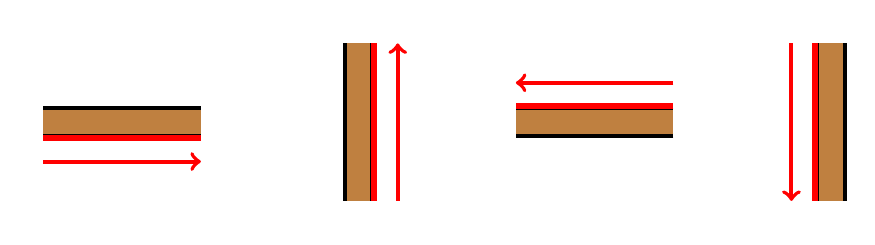
\begin{tikzpicture}
\foreach \n in {0,1,2,3}{
	\MULTIPLY{\n}{90}{\r}
	\MULTIPLY{\n}{3}{\x}
	\begin{scope}[xshift=\x cm,rotate=\r]
	\draw[line width=4mm] (-1,0)--(1,0);
	\draw[line width=3mm,brown] (-1,0)--(1,0);
	\draw[red,line width=.75mm] (-1,-.2)--(1,-.2);
	\draw[red, line width=.5mm,->] (-1,-.5)--(1,-.5);
	\end{scope}
}
\end{tikzpicture}
\caption[Left-to-right along strand]{Foundation chain shown in red, with left-to-right direction along strand indicated by arrow}\label{fig:LtR}
\end{figure}
The next step is to follow the curve around and identify each component. Components are separated by crossings.



\section{Standard Components}
There are four standard components, each of which starts and ends at a dot. A section directly between two dots, with no feature walls, is \textbf{straight}. A single feature wall not touching any other feature walls causes a  \hyperref[sfig:quarterturn]{\textbf{quarter turn}}. Two feature walls meeting at a corner makes a \hyperref[sfig:cornerpoint]{\textbf{point}}, and three feature walls in an open box makes a \hyperref[sfig:twist]{\textbf{twist}}. 

Once you've identified the location on a strand where you want to start, draw a line on one edge.
Follow the segment around until you end up where you started, identifying each component you pass. 
Components are separated by crossings. That is, they will start and stop at dots. Note whether the edge you're following is on the inside or outside of a component (does not apply to straight components).


The right and wrong sides of the strands are basically identical, so it's not crucial to control which side is which. %If you want to, though,
%orient the picture so that segment is horizontal. Draw a line on the bottom of the segment, left-to-right (if you're right-handed). Then the first row (not the foundation chain) will be the right side of the strand.

\begin{figure}[H]\centering
%\begin{subfigure}[t]{.4\textwidth}
%		\centering
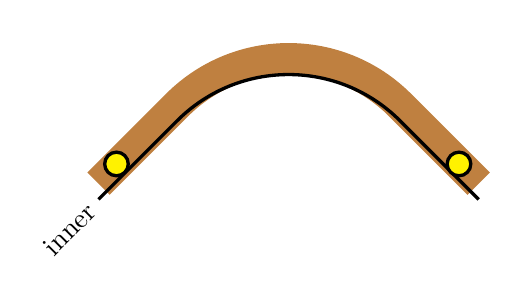
\begin{tikzpicture}%[rotate=90]
\draw[brown,line width=4mm] (0,0) -- (-1,1) arc (45:135:2cm)--+(-1,-1);
\draw[very thick,yshift=-2mm] (0,0) -- (-1,1) arc (45:135:2cm)--+(-1,-1) node[left,rotate=45]{inner};
\draw (-.25,.25)node[bigdot]{};
\draw (-4.6,.25)node[bigdot]{};
\end{tikzpicture}%\end{subfigure}
\hspace{1cm}%
%\begin{subfigure}[t]{.4\textwidth}
%		\centering
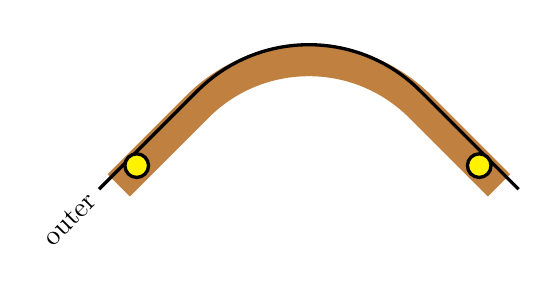
\begin{tikzpicture}%[rotate=90]
\draw[brown,line width=4mm] (0,0) -- (-1,1) arc (45:135:2cm)--+(-1,-1);
\draw[very thick,yshift=2mm] (.25,-.25) -- (-1,1) arc (45:135:2cm)--+(-1.25,-1.25) node[left,rotate=45]{outer};
\draw (-.25,.25)node[bigdot]{};
\draw (-4.6,.25)node[bigdot]{};
\end{tikzpicture}%\end{subfigure}
\caption{Quarter Turn}\label{fig:Q1}
\end{figure}

\begin{figure}[H]
\centering
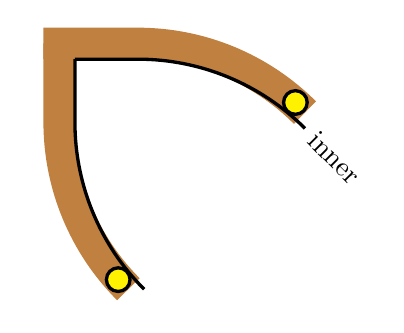
\begin{tikzpicture}%[rotate=90]
\draw[brown,line width=4mm] (-.2,0)--(1,0) arc (90:45:3cm);
\draw[brown,line width=4mm] (0,0)--(0,-1) arc (180:225:3cm);
\draw[very thick,yshift=-2mm] (.2,0)--(1,0) arc (90:45:3cm)node[right,rotate=-45]{inner};
\draw[very thick,xshift=2mm] (0,-.2)--(0,-1) arc (180:225:3cm);
\draw (3,-.75)node[bigdot]{};
\draw (.75,-3)node[bigdot]{};
\end{tikzpicture}
\hspace{1cm}
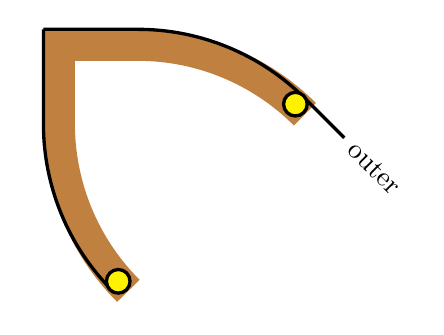
\begin{tikzpicture}%[rotate=90]
\draw[brown,line width=4mm] (-.2,0)--(1,0) arc (90:45:3cm);
\draw[brown,line width=4mm] (0,0)--(0,-1) arc (180:225:3cm);
\draw[very thick,yshift=2mm] (-.2,0)--(1,0) arc (90:45:3cm)--+(.5,-.5)node[right,rotate=-45]{outer};
\draw[very thick,xshift=-2mm] (0,.2)--(0,-1) arc (180:225:3cm);
\draw (3,-.75)node[bigdot]{};
\draw (.75,-3)node[bigdot]{};
\end{tikzpicture}
\caption{Point}\label{fig:P1}
\end{figure}

\begin{figure}[H]
\centering
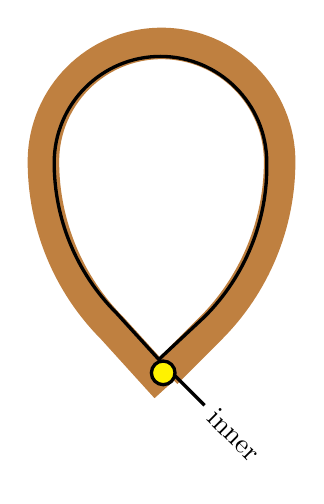
\begin{tikzpicture}[scale=0.75]
\draw[brown,line width=4mm] (-.75,-2.75)--(0,-2) arc (-45:0:4cm) arc (0:180:2cm) arc (180:225:4cm)--(-.75,-3);
(-.2,0)--(1,0) arc (90:45:3cm);
\draw[very thick,xshift=-1mm]  (-.75,-2.5)--(0,-1.8) arc (-45:1:3.6cm) arc (0:180:1.8cm) arc (180:225:3.6cm)--(-.75,-2.55)--+(.75,-.75)node[right,rotate=-45]{inner};
(-.2,0)--(1,0) arc (90:45:3cm);
\draw (-.8,-2.75)node[bigdot]{};
\end{tikzpicture}
\hspace{1cm}
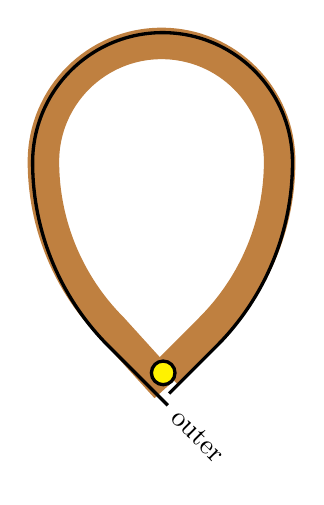
\begin{tikzpicture}[scale=0.75]
\draw[brown,line width=4mm] (-.75,-2.75)--(0,-2) arc (-45:0:4cm) arc (0:180:2cm) arc (180:225:4cm)--(-.75,-3);
\draw[very thick,xshift=1mm,yshift=-1mm](-.8,-3)-- (0,-2.2) arc (-45:0:4.4cm) arc (0:180:2.2cm) arc (180:225:4.4cm)--+(1,-1)node[right,rotate=-45]{outer};
(-.2,0)--(1,0) arc (90:45:3cm);
\draw (-.8,-2.75)node[bigdot]{};
\end{tikzpicture}
\caption{Twist}\label{fig:T1}
\end{figure}
%%%%%%%%%%%%%%%%%%%
\section{Example: Identifying Standard Components}
By way of example, below we identify the components of the \bk.
Below we show this knot with all its dots.

\begin{figure}[H]\centering
\scalebox{0.75}{
\begin{tikzpicture}
\draw (0,0) node{\includegraphics[width=24cm]{border2}};

\foreach \x in {-11,...,11}{
	\foreach \y in {-2,...,2}{
		\ADD{\x}{\y}{\z}
		\ifodd \z
		\else
			\draw (\x,\y)node[bigdot]{};
		\fi
		}}
\foreach \x in {2,6,8,0,-4,-6,-10}{
	\draw (\x,1)--(\x,3);}
\foreach \x in {-8,-6,-2,0,4,6,10}{
	\draw (\x,-1)--(\x,-3);}
\end{tikzpicture}}
\caption{\bk with dots shown\gen}
\end{figure}

A component will follow the strand from one dot to the next. Let's start at the far left of the knot, shown in purple below. We'll trace alone the edge marked in red. Ideally, we like to start at under-crossings where two straight segments meet. So, we start at the red dot.

\begin{figure}[H]\centering
\scalebox{1.25}{
\begin{tikzpicture}
\clip (-12,-3) rectangle (-7.5,3);
\draw (0,0) node{\includegraphics[width=24cm]{border2_1}};

\foreach \x in {-11,...,11}{
	\foreach \y in {-2,...,2}{
		\ADD{\x}{\y}{\z}
		\ifodd \z
		\else
			\draw (\x,\y)node[bigdot]{};
		\fi
		}}
\draw (-10,0)node[bigdot,fill=red]{};
\foreach \x in {2,6,8,0,-4,-6,-10}{
	\draw (\x,1)--(\x,3);}
\foreach \x in {-8,-6,-2,0,4,6,10}{
	\draw (\x,-1)--(\x,-3);}
\end{tikzpicture}}
\caption{End piece of \bk\gen}
\end{figure}
Moving top-to-bottom, our components are as follows: \textcolor{purple}{straight, outer point, straight, outer quarter, inner twist, straight}.

If we were to follow the black edge instead, still moving top-to-bottom, our components would be: straight, inner point, straight, inner quarter, outer twist, straight.
%%%%%%%%%%%%
%%%%%%%%%%%%
Let's move on to the oval part, shown in purple below. We'll trace alone the edge marked in red. Ideally, we like to start at under-crossings where two straight segments meet. So, we start at the red dot.

\begin{figure}[H]\centering
\scalebox{1.25}{
\begin{tikzpicture}
\clip (-12,-3) rectangle (-6,3);
\draw (0,0) node{\includegraphics[width=24cm]{border2_2}};

\foreach \x in {-11,...,11}{
	\foreach \y in {-2,...,2}{
		\ADD{\x}{\y}{\z}
		\ifodd \z
		\else
			\draw (\x,\y)node[bigdot]{};
		\fi
		}}
\draw (-9,-1)node[bigdot,fill=red]{};
\foreach \x in {2,6,8,0,-4,-6,-10}{
	\draw (\x,1)--(\x,3);}
\foreach \x in {-8,-6,-2,0,4,6,10}{
	\draw (\x,-1)--(\x,-3);}
\end{tikzpicture}}
\caption{Oval part of \bk\gen}
\end{figure}
Moving top-to-bottom, our components are as follows: \textcolor{purple}{straight, inner point, straight, straight, straight, inner point, straight, straight}.

If we were to follow the black edge instead, still moving top-to-bottom, our components would be: straight, outer point, straight, straight, straight, outer point, straight, straight.
\medskip

%%%%%%%%%%%%
%%%%%%%%%%%%
Finally, we have the twisted shape, shown in purple below. We'll trace alone the edge marked in red. Ideally, we like to start at under-crossings where two straight segments meet. So, we start at the red dot.

\begin{figure}[H]\centering
\scalebox{1.5}{
\begin{tikzpicture}
\clip (-10.5,-3) rectangle (-1.5,3);
\draw (0,0) node{\includegraphics[width=24cm]{border2_3}};

\foreach \x in {-11,...,11}{
	\foreach \y in {-2,...,2}{
		\ADD{\x}{\y}{\z}
		\ifodd \z
		\else
			\draw (\x,\y)node[bigdot]{};
		\fi
		}}
\draw (-6,0)node[bigdot,fill=red]{};
\foreach \x in {2,6,8,0,-4,-6,-10}{
	\draw (\x,1)--(\x,3);}
\foreach \x in {-8,-6,-2,0,4,6,10}{
	\draw (\x,-1)--(\x,-3);}
\end{tikzpicture}}
\caption{Twisted piece of \bk\gen}
\end{figure}
Moving bottom-to-top along the red edge, our components are as follows: \textcolor{purple}{ straight, straight, inner point, straight, straight, outer twist, straight, straight, inner twist, straight, straight, outer point, straight, straight}.

If we were to follow the black edge instead, still moving bottom-to-top, our components would be: straight, straight, outer point, straight, straight, inner twist, straight, straight, outer twist, straight, straight, inner point, straight, straight.
%%%%%%%%%%%%
%
%[finish me - ugh]
%
%four figures: curved part measures for each corner type
%
%many tables: straight part measures for each pair of corner types; one table for each length of run

%Find the first dot that is \emph{not} on one of your pairs of adjacent parallel lines. If that dot has no feature wall, then this end of your run is simple. Continue in this chapter. If that dot does have a feature wall, then this end is a group run. Go to \ref{ssec:IDgrouprun}.

%To start, you need to know how many feature walls the run has. If the number is odd, then identifying inner and outer sides is done in the obvious way. If the number is even, then use the first bend to identify inner/outer. So an inner twist with an even number of feature walls has an inner first bend and an outer second bend.
%
%\begin{figure}[H]
%\centering
%\begin{tikzpicture}
%\draw[line width=4mm,brown] (0,1)to[bend right](.75,.5)--(6.25,.5)to[bend right](7,1);
%\draw[very thick,yshift=2mm] (0,1)to[bend right](.75,.5)--(6.25,.5)to[bend right](7,1);
%\draw (.5,1.5)node[rotate=-45]{inner};
%\end{tikzpicture}\hspace{1cm}
%\begin{tikzpicture}
%\draw[line width=4mm,brown] (0,1)to[bend right](.75,.5)--(6.25,.5)to[bend right](7,1);
%\draw[very thick,yshift=-2mm] (-.5,1.5)to[bend right](.75,.5)--(6.25,.5)to[bend right](7.5,1.5);
%\draw (-.6,1.)node[rotate=-45]{outer};
%\end{tikzpicture}
%\caption{Simple runs with an odd number of feature walls}
%\end{figure}
%
%
%\begin{figure}[H]
%\centering
%\begin{tikzpicture}
%\draw[line width=4mm,brown] (0,1)to[bend right](.75,.5)--(6.25,.5)to[bend left](7,0);
%\draw[very thick,yshift=2mm] (0,1)to[bend right](.75,.5)--(6.25,.5)to[bend left](7.5,-0.5);
%\draw (.5,1.5)node[rotate=-45]{inner};
%\end{tikzpicture}
%\hspace{1cm}
%\begin{tikzpicture}
%\draw[line width=4mm,brown] (0,1)to[bend right](.75,.5)--(6.25,.5)to[bend left](7,0);
%\draw[very thick,yshift=-2mm] (-.5,1.5)to[bend right](.75,.5)--(6.25,.5)to[bend left](7,-0);
%\draw (-.6,1.)node[rotate=-45]{outer};
%\end{tikzpicture}
%
%\caption{Simple runs with an even number of feature walls}
%\end{figure}
%



%2. identify components (bends, loops, straights, insides and outsides). track around from one edge of the strand. go from dot to dot.


%\section{Group Runs}\label{ssec:IDgrouprun}.
 



%%%%%%%%%%%%%%%%%%%%
\section{Example: Runs}\label{ssec:nomath_run}

When you add parallel adjacent feature walls, the situation gets a lot more complicated. The strand has long straight parts, called \textbf{runs}. Runs start and end at corners. A corner can be one of four types. For identifying the types of corners, see \ref{ssec:drawruns}. The length of a run is the number of dots involved in the parallel lines of feature walls, as in Figure~\ref{fig:featurerun}.

For identifying corner types, remember that C-type, J-type, and L-type corners are named the way they look. D-type corners are direct corners, where the first dot that isn't on the run has no feature wall (as opposed to a perpendicular feature wall). Components start and end at D-type or J-type corners, while C-type and L-type corners connect two runs inside the same component.\medskip

%%%%%%%%%%%%
For practice, we'll identify the corner types and run lengths in the runs of the knot below.

\begin{figure}[H]\centering
\scalebox{.75}{
\begin{tikzpicture}
\draw (0,0) node{\includegraphics[width=16cm]{runs.png}};
\foreach \x in {-8,...,8}{
	\foreach \y in {-4,...,4}{
		\ADD{\x}{\y}{\z}
		\ifodd \z
			\draw (\x,\y)node[bigdot]{};
		\fi
		}}
\draw (-8,-4)rectangle (8,4);
\draw (5,3)-|(-5,-3)-|(3,-1);
\draw (6,2)-|(-4,-2)--(2,-2);
\draw (6,4)--(6,0) (7,3)--(7,-3) (4,0)--(4,-4);
\end{tikzpicture}}
\caption{Example: identifying runs\gen}
\end{figure}

%%%%%%%%%%%%
Let's start with the top, horizontal run, marked in purple below. The adjacent parallel lines of feature walls that define the straight section are highlighted in red.

\begin{figure}[H]\centering
\scalebox{.75}{
\begin{tikzpicture}
\draw (0,0) node{\includegraphics[width=16cm]{runs_1.png}};

\foreach \x in {-8,...,8}{
	\foreach \y in {-4,...,4}{
		\ADD{\x}{\y}{\z}
		\ifodd \z
			\draw (\x,\y)node[bigdot]{};
		\fi
		}}
\draw (-8,-4)rectangle (8,4);
\draw (5,3)-|(-5,-3)-|(3,-1);
\draw (6,2)-|(-4,-2)--(2,-2);
\draw (6,4)--(6,0) (7,3)--(7,-3) (4,0)--(4,-4);
\draw[line width=4pt, red,opacity=0.75] (-6,4)--(6,4) (-5,3)--(5,3);
\draw (-6,3)node[bigdot,fill=red]{};
\draw (6,3)node[bigdot,fill=green]{};
\draw (5,2)node[bigdot,fill=blue]{};

\draw[<-, very thick] (5.75,3.75)--+(1,1)node[above right]{C-type};
\draw[<-, very thick] (-6,3.75)--+(-1,1)node[above left]{D-type};
\end{tikzpicture}}
\caption{D-type and C-type corners\gen}
\end{figure}
%%%%%%%%%%%%
Since there are eleven dots in the walls (6 on top and 5 below), the length of this run is \textbf{11}.

On the left, the red dot is the first dot that is off the run. (If it had a horizontal feature wall, it would extend the run.) Since this dot has no feature wall, that corner is \textbf{D(irect)-type}.

On the right, the green dot is the first dot that is off the run. (If it had a horizontal feature wall, it would extend the run.) This dot has a feature wall perpendicular to the original run, connecting to a feature wall (through the blue dot) parallel to the original feature wall. So the right corner of the run is \textbf{C-type}. Notice how the run makes a 180 degree (C-shaped) turn into a new run. 
\medskip



%%%%%%%%%%%%

Let's continue to the next run, marked in purple below. The adjacent parallel lines of feature walls that define the straight section are highlighted in red.

%%%%%%%%%%%%


\begin{figure}[H]\centering
\scalebox{.75}{
\begin{tikzpicture}
\draw (0,0) node{\includegraphics[width=16cm]{runs_2.png}};

\foreach \x in {-8,...,8}{
	\foreach \y in {-4,...,4}{
		\ADD{\x}{\y}{\z}
		\ifodd \z
			\draw (\x,\y)node[bigdot]{};
		\fi
		}}
\draw (-8,-4)rectangle (8,4);
\draw (5,3)-|(-5,-3)-|(3,-1);
\draw (6,2)-|(-4,-2)--(2,-2);
\draw (6,4)--(6,0) (7,3)--(7,-3) (4,0)--(4,-4);
\draw[line width=4pt, red,opacity=0.75] (-4,2)--(6,2) (-5,3)--(5,3);
\draw (-5,2)node[bigdot,fill=red]{};
\draw (-4,1)node[bigdot,fill=green]{};


\draw[<-, very thick] (-4.75,2.75)--+(-2,2)node[above left]{L-type};
\end{tikzpicture}}
\caption{L-type corner\gen}
\end{figure}
%%%%%%%%%%%%
There are 10 dots in the adjacent parallel lines of feature walls (5 each on the top and bottom), so we call the length of this run \textbf{10}. The first dot on the left that is \textit{not} a part of these lines is marked in red.  (We know it's the first one off the run because if it had a horizontal feature wall, it would extend the run). It has a feature wall that is perpendicular to the original run. The dot after that is marked in green. It has a feature wall that is also perpendiculat to the original run. That makes this an \textbf{L-type corner}. Note the strand makes a right angle, like the letter L.
\medskip

%%%%%%%%%%%%
Continuing along the component, we come to a vertical run, marked in purple below. The adjacent parallel lines of feature walls are in red.
%%%%%%%%%%%%


\begin{figure}[H]\centering
\scalebox{.75}{
\begin{tikzpicture}
\draw (0,0) node{\includegraphics[width=16cm]{runs_3.png}};

\foreach \x in {-8,...,8}{
	\foreach \y in {-4,...,4}{
		\ADD{\x}{\y}{\z}
		\ifodd \z
			\draw (\x,\y)node[bigdot]{};
		\fi
		}}
\draw (-8,-4)rectangle (8,4);
\draw (5,3)-|(-5,-3)-|(3,-1);
\draw (6,2)-|(-4,-2)--(2,-2);
\draw (6,4)--(6,0) (7,3)--(7,-3) (4,0)--(4,-4);
\draw[line width=4pt, red,opacity=0.75] (-5,3)--(-5,-3) (-4,2)--(-4,-2);
\draw (-4,-3)node[bigdot,fill=red]{};
\draw (-3,-2)node[bigdot,fill=green]{};


\draw[<-, very thick] (-4.5,-2.75)--+(-2,-2)node[below left]{L-type};
\end{tikzpicture}}
\caption{L-type corner\gen}
\end{figure}
%%%%%%%%%%%%
The length of the run is \textbf{5}. Just like the last one, this is an \textbf{L-type} corner.
%%%%%%%%%%%%
\medskip

The component ends with another horizontal run. That run is in purple below, and its parallel lines of feature walls are in red.
%%%%%%%%%%%%


\begin{figure}[H]\centering
\scalebox{.75}{
\begin{tikzpicture}
\draw (0,0) node{\includegraphics[width=16cm]{runs_4.png}};

\foreach \x in {-8,...,8}{
	\foreach \y in {-4,...,4}{
		\ADD{\x}{\y}{\z}
		\ifodd \z
			\draw (\x,\y)node[bigdot]{};
		\fi
		}}
\draw (-8,-4)rectangle (8,4);
\draw (5,3)-|(-5,-3)-|(3,-1);
\draw (6,2)-|(-4,-2)--(2,-2);
\draw (6,4)--(6,0) (7,3)--(7,-3) (4,0)--(4,-4);
\draw[line width=4pt, red,opacity=0.75] (-5,-3)--(3,-3) (-4,-2)--(2,-2);
\draw (3,-2)node[bigdot,fill=red]{};
\draw (2,-1)node[bigdot,fill=green]{};

\draw[<-, very thick] (2.75,-2.75)--+(2,-2)node[below right]{J-type};
\end{tikzpicture}}
\caption{J-type corner\gen}
\end{figure}
%%%%%%%%%%%%
The length of this run is \textbf{7}. The first dot not on the run is marked in red. (We know it's the first one off the run because if it had a horizontal feature wall, it would extend the run). It has a feature wall perpendicular to the original run, so we move to the next dot, shown in green. This has no feature wall, so the corner is \textbf{J-type}. (Note the curve made by the strand approximates a letter J.) The component ends at the green dot.
%%%%%%%%%%%%
\medskip

The full component (from crossing to crossing) is shown in purple below. It can be described as follows, starting in its upper-left corner: \textcolor{purple}{D-type corner, run of length 11, C-type corner, run of length 10, L-type corner, run of length 5, L-type corner, run of length 7, J-type corner}. 
%%%%%%%%%%%
\begin{figure}[H]\centering
\scalebox{.75}{
\begin{tikzpicture}
\draw (0,0) node{\includegraphics[width=16cm]{runs_5.png}};

\foreach \x in {-8,...,8}{
	\foreach \y in {-4,...,4}{
		\ADD{\x}{\y}{\z}
		\ifodd \z
			\draw (\x,\y)node[bigdot]{};
		\fi
		}}
\draw (-8,-4)rectangle (8,4);
\draw (5,3)-|(-5,-3)-|(3,-1);
\draw (6,2)-|(-4,-2)--(2,-2);
\draw (6,4)--(6,0) (7,3)--(7,-3) (4,0)--(4,-4);
\end{tikzpicture}}
\caption{One component with four runs\gen}
\end{figure}
%%%%%%%%%%%%

Similarly, the component shown in red below can be described (starting from the left) as \textcolor{red}{D-type corner, run of length 4, C-type corner, run of length 7, J-type corner}.
%%%%%%%%%%%
\begin{figure}[H]\centering
\scalebox{.75}{
\begin{tikzpicture}
\draw (0,0) node{\includegraphics[width=16cm]{runs_6.png}};

\foreach \x in {-8,...,8}{
	\foreach \y in {-4,...,4}{
		\ADD{\x}{\y}{\z}
		\ifodd \z
			\draw (\x,\y)node[bigdot]{};
		\fi
		}}
\draw (-8,-4)rectangle (8,4);
\draw (5,3)-|(-5,-3)-|(3,-1);
\draw (6,2)-|(-4,-2)--(2,-2);
\draw (6,4)--(6,0) (7,3)--(7,-3) (4,0)--(4,-4);
\end{tikzpicture}}
\caption{One component with two runs\gen}
\end{figure}
%%%%%%%%%%%%


%%%%%%%%%%%%

\section{Number Intersections}

In order to assemble the strands once they're done, it's helpful to number intersections. 

Follow your strand around as you did when you were identifying components. Between each component, add a labelled marker with the number of the intersection, noting whether that part of the strand is on the top or the bottom of the intersection.

Often knots are symmetric in such a way that different strands can be crocheted using the same instructions. If you're planning on doing this, when you number intersections along one strand, number them along all the strands. This will probably result in several intersections having the same number. The intersection labels are helpful for assembling your final knot, but slightly ambiguous labelling is usually easy enough to deal with by carefully following your knot diagram.


%%%%%%%%%%%%%%%
\section{Components to Patterns}
%%%%%%%%%%%%%%%
Now we have a way of breaking down a knot into a sequence of components. Each component has its own pattern. So the task now is to simply match them up. If you want to make a point, you can look up the pattern for a point; then if you want to attach it to a quarter turn, look up the pattern for a quarter turn. 

There's a lot of finagling involved:  the order of the components reverses every row since we go back and forth; you need to keep track of which row you're in, and whether you're working outside-to-inside or inside-to-outside along a turn; and you need to remember which marker goes where.  This is \textit{definitely} the kind of grunt work best outsourced to a computer.

\subsection{How to do it all by hand} If you don't want to use the program to assemble your list of components into a pattern, you can just look up the dimensions of each component. Stitch counts for components are given in Appendix sections  \ref{Asec:stitchcounts} (standard components) and \ref{Asec:runcount} (runs). 

For example, suppose your strand has three components: straight, inner quarter, outer quarter. Let the markers between them be 1T and 2B.


%%%%%%%%%%%%
\begin{figure}[H]\centering
\begin{tikzpicture}
\draw[line width=4mm] (0,0) -- (1.3,1.3) arc (135:45:1cm)--+(.3,-.3) coordinate(2){};
\draw[line width=4mm]  (2)--+(.3,-.3)arc (225:315:1cm)--+(.3,.3) ;
\draw[line width=3mm,red,yshift=-.5mm] (0,0) -- (1.3,1.3) arc (135:45:1cm)--+(.3,-.3) coordinate(2){};
\draw[line width=3mm,red,yshift=-.5mm]  (2)--+(.3,-.3)arc (225:315:1cm)--+(.3,.3) ;
\draw[line width=3mm,brown] (0,0) -- (1.3,1.3) arc (135:45:1cm)--+(.3,-.3) coordinate(2){};
\draw[line width=3mm,brown]  (2)--+(.3,-.3)arc (225:315:1cm)--+(.3,.3) ;
\draw (1,1) node[shape=circle,fill=white, fill opacity=0.5,draw]{1};
\draw (2) node[shape=circle,fill=white, fill opacity=0.5,draw]{2};
\draw[red] (.7,.2)node[]{S};
\draw[red] (2,1.4)node[below]{IQ};
\draw[red] (4,.3)node[below]{OQ};
\end{tikzpicture}
\caption{Example strand}
\end{figure}
%%%%%%%%%%%%

\begin{description}
\item[Foundation Chain] We see that each straight component has 10 stitches (Figure~\ref{fig:S}); the innermost row of a quarter turn has 3  sts / 7 sts / 3 sts (Figure~\ref{fig:Q}); and the outermost row of a quarter turn has 3 sts / 15 sts / 3 sts (Figure~\ref{fig:Q}. So our foundation chain is:
\begin{center}
10 ch /(1T) 3 ch / 7 ch / 3 ch /(2B) 3 ch / 15 ch / 3 ch
\end{center}
\item[Row 1] Now we're going back in the other direction, so we \textit{start} with the outer quarter. Moving in one row from the outside, we see it has lengths 3 / 14 / 3, and that 14 is one less than 15, the previous measure (Figure~\ref{fig:Q}). Then we go to the inner quarter turn, which has measures 3 / 8 (+1) / 3 (Figure~\ref{fig:Q}). Finally, the straight section always has 10 sts (Figure~\ref{fig:S}). Ignoring the labels, we have these directions:
\begin{center}
3 sc / 14 sc (-1) / 3 sc / 3 sc / 8 sc (+1) / 3 sc / 10sc
\end{center}
\end{description}

Continue like this until you've finished all rows.

\subsection{How to avoid doing it all by hand}\label{ssec:Python}
In an ideal world, I'd make a nifty web app that goes straight from the picture to the pattern. In the real world, even after going through a million tutorials that say it's \textit{soooo easy}, I'm still clueless. Sorry. So what I have instead is some utilitarian Python in a Jupyter notebook. You enter the knot and your dimensions, and the program gives you a pattern. 

I've tested it on a number of patterns, but of course there may still be mistakes. All it does it automate the process of finding and concatenating arclengths, so if something looks wrong, it's easy enough to spot-check by hand.
\medskip


\subsubsection*{How to open the notebook}
If you know what a Jupyter notebook is and how to open it, you can grab it directly from the github repository here: \url{https://github.com/ecyeager/KnotworkCrochet}\quad It's formatted to be as user-friendly as possible for people uncomfortable with programming. If you know even a little Python, you can get rid of a lot of parts. For example, it's nicer to hard-code variables like stitch height than it is to enter them with widgets, so you can update that variable in the appropriate code cell and then just delete its widget.

If you're not so sure about Jupyter but you still want to give things a try, click here: \url{https://mybinder.org/v2/gh/ecyeager/KnotworkCrochet/main}\quad This uses Binder, which is a fancy way of being able to do all your code stuff in your browser, without having to install programs on your computer.

It will take a few minutes to load. Once it's loaded, you'll see a screen that looks something like this:
\begin{figure}[H]
\includegraphics[width=\textwidth]{pic/binder}
\caption{Binder screen}
\end{figure}

Click on the first file, PatternGeneratorPublic.ipynb.  That will load up the Jupyter notebook, which will look something like this (but longer):

\begin{figure}[H]
\includegraphics[width=\textwidth]{pic/notebook}
\caption{Notebook}
\end{figure}


\subsubsection*{How to use the notebook}
There are alternating cells of text and code. Each code cell is run by clicking somewhere inside it and then pressing shift+enter. The text generally tells you what to do. 

\subsubsection*{What to do if you know absolutely no coding}
Start by clicking on the cell that starts with ``\#Imports" and then hitting shift+enter. You should see some buttons and text fields pop up below that cell (Figure~\ref{fig:defaults}. The defaults for your knot dimensions are pre-filled, which you can change as you like. (You might have to scroll to see all the options.)

\begin{figure}[H]\centering
\includegraphics[width=.75\textwidth]{pic/defaults}
\caption{Buttons and text fields for entering dimensions}\label{fig:defaults}
\end{figure}

 Move from each cell to the next, following the directions. Instructions should guide you through the process. Make sure you hit shift+enter for each cell with code in it.\medskip

The hardest part of the notebook is describing the knot in a way the program will understand. There are buttons to do this for you.


\begin{figure}[H]\centering
\includegraphics[width=.5\textwidth]{pic/buttons}
\caption{Buttons for entering the knot pattern}
\end{figure}

If your strand has components (say) ``straight, straight, outer quarter turn," then click on those buttons, one-by-one, in that order. If you want to add a run, select the corner types and lengths, then click "add run." (Unfortunately I only have buttons for runs with D-type and J-type corners -- not for runs that are concatenated with C-type or L-type corners.)

If you'd also like to add labelled stitch markers, then you can enter them one-by-one in the next cell. Remember to hit shift+enter to make the entry box appear.

\begin{figure}[H]\centering
\includegraphics[width=.75\textwidth]{pic/markers}
\caption{Text box for entering the markers}
\end{figure}

One by one, enter the label you'd like for a marker, then click ``add label." 

\subsubsection{What to do if you know some coding}
First, remember that we all started somewhere, and try not to get too annoyed at my lack of coding elegance. Feeling generous? OK, let's move on.\medskip

Using the widgets is harder than hard-coding the variables, not least because with the widgets you can't easily save your work. So I recommend just reading the comments and changing parameters in the code cells.

The hardest things to enter are the lists ``pattern" and ``markers."
\begin{description}
\item[pattern] This is a list whose entries are components OR customized lists of instructions. You'll add them in order, as you go along your strand.
\begin{description}
\item[standard components]
If you have a standard component, enter a string: S, IQ, OQ, IP, OQ, IT, or OT (straights, inner/outer quarter turns, inner/outer points, and inner/outer twists).
\item[custom instructions] If you enter anything other than the seven strings above, it needs to be a list with one entry per row (including the foundation row). So you can have an element of the list ``pattern" be a list of the form: \texttt{["instructions for row 0","instructions for row 1",...]}

If you happen to have a run, there's a separate function that will define these instructions for you.
\item[run] The function ``run" takes a list as an argument. That list should have elements that alternate between corner types (ID, OD, IJ, OJ, IC, OC, IL, OL, entered as strings) and lengths (entered as numbers). 

For example, suppose a run starts with an inner D-type corner, then has straight length 5, then has an inner C-type corner, then straight length 4, then an outer J-type corner. To generate the instructions for that run, you would use \texttt{run(["ID",5,"IC",4,"OJ"])}
\item[Example]
Suppose a strand has the following components:
\begin{center}
straight, inner quarter, straight, inner D-type corner, run of length 3, inner J-type corner, straight
\end{center}
Then you would define this list:
\begin{center}
\texttt{pattern=["S","IQ","S",run(["ID",3,"IJ"]),"S"]}
\end{center}
Note that the run is not entered as a string.
\end{description}
\item[markers] To add stitch markers to the crochet instructions, define ``markers" as a list of strings. For example, \begin{center}\texttt{markers=["1T","2B","3T","4B"]}\end{center}

\end{description}
Remember that you basically run every cell. If you go back and change something at the front, you'll probably have to re-run at least some cells in order for everything to update. The final cell in the notebook will turn your pattern and parameters into crochet instructions. 
%%%%%%%%%%%%%%%

%%%%%%%%%%%%%%%%%%%%%%%%%%
\chapter{Translating Knots to Crochet, Part 2}\label{sec:math}
%%%%%%%%%%%%%%%%%%%%%%%%%%
\summ{Math in this part. An explanation of the work behind the patterns in the Chapter~\ref*{sec:nomath}. %If you want to change the basic shapes to suit your own needs, this is the place to look. For example, if you want to make your twists pointy instead of smooth, or 
}

In this chapter, we detail the exact shapes assigned to each component. We only use high-school-level geometry, but we use a lot of it.

%Two considerations determine the fundamental proportions in your work: your gauge when working single crochets, and the dimensions you'd like for your strand. These are discussed in \ref{ssec:gauge}.

%Knots made following the method in Chapter~\ref{sec:making} consist of various components: straight lines, quarter turns, points, twists, and runs. The first four are considered ``standard components," found in \ref{ssec:parts}. Runs are covered in \ref{ssec:parts_runs}.


\section{Underlying Dimensions: Gauge and Strand Width}\label{ssec:gauge}

It is common in crochet patterns to assume that a single crochet is roughly square. That is, if you work a swatch of 10 sc for 10 rows, it should be as long as it is wide. %For most patterns, this assumption is close enough to the truth that everything works fine. 
For these patterns, we use slightly more precision.

We will treat the width of a sc stitch as one unit. The height is generally less than one unit. To measure your stitch height, work a swatch in sc with, adding rows until it is a square. 

A good size to start with is 10 sc worked for 10 rows; keep adding rows until the height is as equal as possible. If you want increased accuracy, try 20 sc. If you don't have a measuring tape handy, you can check whether a rectangle is a square by folding it diagonally, explained in Figures~\ref{fig:rect} and \ref{fig:square}.

\begin{figure}[H]
\begin{subfigure}[t]{.4\textwidth}
		\centering
\begin{tikzpicture}
\filldraw[thick,fill=yellow] (0,0) rectangle (4,3);
\draw[line width=4pt,red] (0,3)|-(4,0);
\draw (0,0)node[bigdot]{};
\end{tikzpicture}
\caption{Fold the swatch at the corner dot so that the red lines align.}
\end{subfigure}\hfill
%
\begin{subfigure}[t]{.4\textwidth}
		\centering
\begin{tikzpicture}
\filldraw[thick,fill=yellow] (3,0)rectangle (4,3);
\draw[fill=yellow!50!green] (0,0)--(3,3)|-cycle;
\draw[line width=4pt,red] (0,0)--(3,0);
\draw[line width=2pt,red] (3.1,0)--(4,0);
\draw (0,0)node[bigdot]{};
\end{tikzpicture}
\caption{The section sticking out on the right tells you this is not yet square. Work more rows.}
\end{subfigure}
\caption{Folding a Rectangle}\label{fig:rect}
\end{figure}
%-----

\begin{figure}[H]
\begin{subfigure}[t]{.4\textwidth}
		\centering
\begin{tikzpicture}
\filldraw[thick,fill=yellow] (0,0) rectangle (3,3);
\draw[line width=4pt,red] (0,3)|-(3,0);
\draw (0,0)node[bigdot]{};
\end{tikzpicture}
\caption{Fold the swatch at the corner dot so that the red lines align.}
\end{subfigure}\hfill
%
\begin{subfigure}[t]{.4\textwidth}
		\centering
\begin{tikzpicture}
\draw[fill=yellow!50!green] (0,0)--(3,3)|-cycle;
\draw[line width=4pt,red] (0,0)--(3,0);
\draw (0,0)node[bigdot]{};
\end{tikzpicture}
\caption{When you align the two red sides, the remaining two sides line up as well. You have made yourself a square.}
\end{subfigure}
\caption{Folding a Square}\label{fig:square}
\end{figure}
%-----


The ratio $\frac{\text{number of sc per row}}{\text{number of rows}}$ is your \textbf{stitch height}. It will probably be less than 1. For the example patterns, I have used my own stitch height, which is $\frac{60}{69}$. (I worked a swatch 30 sc wide; 34 rows was a little shorter than a square, and 35 was a little longer. So I called my stitch height $\frac{30}{34.5}$.)

\begin{figure}[H]\centering
\begin{tikzpicture}[scale=0.2]
\COPY{.3}{\a}
\foreach \x in {1,...,30}{
	\foreach \y in {1,...,34}{
		\draw[yscale=30/34] (\x+\a,\y+\a)--(\x-\a,\y-\a)  (\x-\a,\y+\a)--(\x+\a,\y-\a);}}
\end{tikzpicture}
\caption{If 30 sc and 34 rows makes a square, then stitch height is $\frac{30}{34}$.}
\end{figure}


The lengths of segments in a strand are determined by the \textbf{dot-to-dot distance}. This is the distance, in stitches, between two diagonally-adjacent dots. So a straight section will have this many stitches in it.

The width of a strand works nicely as an even number. Taking into account the foundation chain, even numbers make the middle of the strand easy to find.

\begin{figure}[H]\centering
\begin{tikzpicture}
\begin{scope}[opacity=0.4]
\foreach \y in {0,...,6}{
	\draw (0,\y/2)--(5,\y/2)node(s\y){};}
\foreach \x in {0,0.5,...,4.5}
	{\draw (\x+.25,-0.1)node[shape=ellipse,inner sep=0,minimum width=4mm, minimum height=1mm, draw]{};
	\foreach \y in {0,...,5}{
		\draw(\x,\y/2)--+(.4,.45);
		\draw (\x+.4,\y/2)--+(-.4,.45);}}
\end{scope}
\draw (s0) node[right]{foundation chain};
\draw (s3) node[right]{row 3 (middle of strand)};
\foreach \y in {1,2,4,5,6}{
	\draw (s\y)node[right]{row \y};}

\end{tikzpicture}
\caption{Even number of rows in a strand}
\end{figure}
%%%%%%%%%%%%

If the width of a strand is one-half its dot-to-dot distance, then the spaces between strands will be as thick as the strand itself in a plain knot. For heavier items, like afghan squares, a thicker strand will make sense. The strand width must be less than the dot-to-dot distance.

\begin{figure}[H]\centering
\begin{subfigure}[t]{.475\textwidth}
		\centering
\begin{tikzpicture}[scale=0.9]
\COPY{1.414}{\u}
\COPY{.5}{\ep}
\SUBTRACT{2}{\ep}{\aa}
\MULTIPLY{\aa}{\u}{\l}
\DIVIDE{\l}{2}{\halfl}
\MULTIPLY{\u}{\ep}{\w}
\DIVIDE{\w}{2}{\halfw}
\foreach \x in {2,4}{
	\foreach \y in {0,2}{\filldraw[fill opacity=0.1,xshift=\x cm,yshift=\y cm,rotate=-45] (-\halfl,-\halfw) rectangle (\halfl,\halfw);
	\draw(\x,\y)node[bigdot]{};}}
\foreach \x in {1,3,5}{
\foreach \y in{1,3}{\filldraw[fill opacity=0.1,xshift=\x cm,yshift=\y cm,rotate=45] (-\halfl,-\halfw) rectangle (\halfl,\halfw);
\draw(\x,\y)node[bigdot]{};}}
\end{tikzpicture}
\caption{Strand width one-half of the dot-to-dot distance}
\end{subfigure}\hfill%%
\begin{subfigure}[t]{.475\textwidth}
		\centering
\begin{tikzpicture}[scale=0.9]
\COPY{1.414}{\u}
\COPY{.67}{\ep}
\SUBTRACT{2}{\ep}{\aa}
\MULTIPLY{\aa}{\u}{\l}
\DIVIDE{\l}{2}{\halfl}
\MULTIPLY{\u}{\ep}{\w}
\DIVIDE{\w}{2}{\halfw}
\foreach \x in {2,4}{
	\foreach \y in {0,2}{\filldraw[fill opacity=0.1,xshift=\x cm,yshift=\y cm,rotate=-45] (-\halfl,-\halfw) rectangle (\halfl,\halfw);
	\draw(\x,\y)node[bigdot]{};}}
\foreach \x in {1,3,5}{
\foreach \y in{1,3}{\filldraw[fill opacity=0.1,xshift=\x cm,yshift=\y cm,rotate=45] (-\halfl,-\halfw) rectangle (\halfl,\halfw);
\draw(\x,\y)node[bigdot]{};}}
\end{tikzpicture}
\caption{Strand width two-thirds of the dot-to-dot distance}
\end{subfigure}
\caption{Strand widths}
\end{figure}

%For particularly chunky dimensions, you might find some quantities below end up being negative. The insides of corners might have to be dealt with on an ad-hoc basis.


%%%%%%%%%%%%%%%%%%
\section{Restrictions}

The general dimensions you need to decide on are:
\begin{description}
\item[$\mathbf u$:] This is the dot-to-dot distance, also the number of stitches in a straight segment.
\item[$\mathbf s$:] This is the straight section on either end of the arc when you work a quarter-turn. Applies only if your knot has quarter turns. (It probably does.)
\item[$\mathbf t$:] This is the straight section added to a twist. Only applies if your knot has a twist (and you want it a little elongated).
\item[strand width:] This is the total width of one strand. It's the number of rows in the piece multiplied by your stitch height. This isn't given a variable explicitly elsewhere, but for now let's call it $w$. The largest value of $\Delta$ (used later on as the distance away from the centre of the strand) is $\frac{w}{2}$.
\end{description}

In order to keep your knot from unintentionally overlapping itself, these dimensions have certain restrictions. For each component, I calculated the relationships between dimensions that will keep the component from crossing its feature wall(s). These are given in Table~\ref{table:restrictions}.

If a component does not appear in your knot, then it is possible to ignore the restriction. Since your actual knot is unlikely to match the planned dimensions exactly, it's nice to build in some error tolerance. If you violate a restriction, you can probably fix the relevant parts of your pattern by hand.
%%%%%%%%%%%%
\begin{table}[H]
\centering
{\renewcommand{\arraystretch}{1.2}
\begin{tabular}{|m{0.15\linewidth} |  m{0.3\linewidth} | m{0.5\linewidth} | }
\hline 
component(s) & restriction & notes\\ \hline
\hyperref[sssec:straight]{straight} &\centering $w\le u$ & You'll want to keep away from $w=u$, unless you specifically want your strands to bunch up.\\ \hline
\hyperref[sssec:quarter]{quarter turn} &\centering  $s  \leq u - (\sqrt2+1)\frac{w}{2}$ & The value of $s$ has a huge impact on how your quarter turns look. Bigger $s$-values make a more dramatic arc.\\ \hline
\hyperref[sssec:point]{point} & \centering $w \le u \left(2-\sqrt 2\right)\cdot(\text{stitch height})$
% $ u\left(2-\sqrt 2\right) \ge \text{\small (number of rows in a strand)}$ 
&
If we take the number of rows as $\frac{w}{\text{stitch height}}$, this is equivalent to 
 $\text{ (number of rows in a strand)} \le u\left(2-\sqrt 2\right) $
 %$w \le u \left(2-\sqrt 2\right)\cdot(\text{stitch height})$. \\ \hline
% \hyperlink{sssec:point}{point} & $w \le u\left(2\sqrt 2 - 2 \right)$ &
 \\\hline
\hyperref[sssec:twist]{twist} &\centering  ${ w  \leq u\left(2\sqrt 2 - 2\right)}$ and 
${t\leq\left(\sqrt 2 - 1\right)u-\frac{w}{2}}$ & Remember this causes a dangly piece, so consider the final use of your object before you make a knot with these components.  \\ \hline
\raggedright
\hyperref[sssec:j]{J-type} and \linebreak\hyperref[sssec:c]{C-type} corners & \centering $w  \leq \frac{u}{\sqrt 2}$  & Have I mentioned yet that runs are a pain in the neck?\medskip

 If your J-type or C-type corner is at the outside edge of the piece, then there's nothing for it to run into, so this is somewhat easier to ignore.\medskip 

You can also reduce the length of the attached runs to pull a corner away from an overrun feature wall. \\ \hline
\end{tabular}}
\caption{Restrictions on dimension parameters}\label{table:restrictions}
\end{table}%%%%%%%%%%%%
%%%%%%%%%%%%
%%%%%%%%%%%%%%%%%%
\section{Side Length}

Note that the distance between two dots that are \emph{horizontally} (or vertically) adjacent is the square root of 2 times the dot-to-dot distance.

\begin{figure}[H]\centering\hfill
\foreach \straight in {.8}{
\begin{tikzpicture}[rotate=90]
\COPY{2.828}{\u}%dtd
\COPY{\straight}{\s}%straight
\DIVIDE{\s}{1.414}{\sx}%straight/sqrt 2
\SUBTRACT{\u}{\s}{\rad}

\foreach \y in {0,4}{
\begin{scope}[yshift=\y cm]
\draw (4,0)node[bigdot]{};
\draw (2,-2)node[bigdot]{};
\draw (2,2)node[bigdot]{};
\foreach \del in {.5,0,-.5}{
\DIVIDE{\del}{1.414}{\dx}
\ADD{\rad}{\del}{\radius}
\draw[ultra thick] (2+\dx,-2-\dx)--(2+\sx+\dx,-2+\sx-\dx) arc (-45:45:\radius cm)--+(-\sx,\sx);
\draw[ultra thick] (2+\dx,2+\dx)--(2+\dx+\sx,2+\dx-\sx);
\draw[ultra thick] (2+\dx,-2-\dx)--(2+\sx+\dx,-2+\sx-\dx);
}
\end{scope}}

\draw[|-|, very thick] (4.5,0)--(4.5,4)node[midway,above]{$\sqrt 2 \cdot u$};
\end{tikzpicture}\hfill}
\caption{Border Measure}
\end{figure}

So if your dot-to-dot distance is, say, 10 stitches, then the number of stitches between peaks on your border will be about 14, since $10\sqrt 2 \approx 14$. 

This is useful for planning the final dimensions of a piece, or for adding a straight border.



\section{Component Geometry}\label{ssec:parts}
Crossings occur at dots, where the strands should meet at right-angles to one another. So given our usual orientation, we can assume every segment starts and ends at a dot, with initial and final angles 45 or -45 degrees.

In general we will denote by $u$ (for ``unit") the dot-to-dot length, and we assume the stitch width is 1. That way, length and arclength are measured in stitches.

Each row has height equal to the stitch height; we will use the shorthand $\Delta$ for the amount added or subtracted from the middle row. So for the middle row, $\Delta=0$; for the row before resp. after the middle row, $\Delta = -(\text{stitch height})$ resp.  $\Delta = +(\text{stitch height})$; etc.

Segments are broken down into straight pieces, right angles, and curves. Curves are worked as arcs of circles. This way we can work our increases uniformly throughout the curve, and easily compute arclength.


\subsection{Straight}\label{sssec:straight}
All rows have the same length on a straight segment: the dot-to-dot length, $u$.
\begin{figure}[H]\centering
\begin{tikzpicture}[scale=0.8]
\draw (0,0)node[bigdot]{};
\draw (5,5)node[bigdot]{};
\foreach \y in {-1,0,1}{
	\draw (-\y,\y)--(5-\y,5+\y)node[xshift=4mm,yshift=4mm](s\y){$u$};}
\draw[|-|] (-.5,-.5)--(.5,-1.5)node[midway,left,rotate=45]{$\Delta$};
\end{tikzpicture}
\caption{Straight segment}
\end{figure}
\subsection{Quarter Turn}\label{sssec:quarter}

Using a quarter-circle for a quarter-turn in a knot results in a fairly flat, uninspiring curve. To make the curve more pronounced, the segment begins and ends with a short straight section.

\begin{figure}[H]\centering\hfill
\foreach \straight in {.2,.8,1.4}{
\begin{tikzpicture}
\COPY{2.828}{\u}%dtd
\COPY{\straight}{\s}%straight
\DIVIDE{\s}{1.414}{\sx}%straight/sqrt 2
\SUBTRACT{\u}{\s}{\rad}
\draw (4,0)node[bigdot]{};
\draw (2,-2)node[bigdot]{};
\draw (2,2)node[bigdot]{};
\draw (4,-1.5)--(4,1.5);
\foreach \del in {.5,0,-.5}{
\DIVIDE{\del}{1.414}{\dx}
\ADD{\rad}{\del}{\radius}
\draw[ultra thick,black] (2+\dx,-2-\dx)--(2+\sx+\dx,-2+\sx-\dx) arc (-45:45:\radius cm)--+(-\sx,\sx);
\draw[ultra thick,red] (2+\dx,2+\dx)--(2+\dx+\sx,2+\dx-\sx);
\draw[ultra thick,red] (2+\dx,-2-\dx)--(2+\sx+\dx,-2+\sx-\dx);
}
\end{tikzpicture}\hfill}
\caption[Quarter turns with straight sections]{Quarter turns with straight segments of varying lengths shown in red}
\end{figure}


Let the length of the straight segment be $s$. This is the same for all rows. The radius of the quarter-turn is $u-s+\Delta$, so the arclength of the quarter-circle segment is $\frac{\pi}{2}\left(u-s+\Delta\right)$.

\begin{figure}[H]\centering
\begin{tikzpicture}
\COPY{2.828}{\u}
\draw[ultra thick,red] (2,-2)--(3,-1)node[midway,below,rotate=0]{$s$};
\draw[ultra thick,red] (2,2)--(3,1)node[midway,above,rotate=-0]{$s$};
\draw[ultra thick,black,|-|] (3,1) arc (45:-45:1.414cm)node[midway,right]{$\frac{\pi}{2}\left(u-s+\Delta \right)$};
\end{tikzpicture}
\caption{Quarter turn lengths}
\end{figure}
%%%%%%%%%%%%
%%%%%%%%%%%%
%%%%%%%%%%%%
\newcommand{\xcoord}[3]{
\SUBTRACT{#2}{.1}{\y}
\ADD{#2}{.1}{\yy}
\draw (#1,\yy)--(#1,\y)node[below]{#3};}
%
\begin{figure}[H]\centering
\begin{tikzpicture}[scale=1.5]
\COPY{2.828}{\u}%dtd
\DIVIDE{\u}{1.414}{\ux}
\COPY{1.}{\s}%straight
\DIVIDE{\s}{1.414}{\sx}%straight/sqrt 2
\COPY{.5}{\del}%Delta
\DIVIDE{\del}{1.414}{\dx}
\SUBTRACT{\u}{\s}{\rad}
\draw (4,0)node[bigdot]{};
\draw (2,-2)node[bigdot]{};
\draw (2,2)node[bigdot]{};
\draw (4,-1.5)--(4,1.5);
\foreach \d in {0,\del,-\del}{
\DIVIDE{\d}{1.414}{\dx}
\ADD{\rad}{\d}{\radius}
\draw[ultra thick,black] (2+\dx,-2-\dx)--(2+\sx+\dx,-2+\sx-\dx) arc (-45:45:\radius cm)--+(-\sx,\sx);
\draw[ultra thick,red] (2+\dx,2+\dx)--(2+\dx+\sx,2+\dx-\sx);
\draw[ultra thick,red] (2+\dx,-2-\dx)--(2+\sx+\dx,-2+\sx-\dx);
}

\draw[<->] (1,-3) -- (5,-3);

\begin{scope}[xshift=2cm,yshift=-3cm]
\xcoord{0}{0}{0}
\xcoord{\ux}{0}{$\frac{u}{\sqrt 2}$}
\draw[|-|,black] (0,.5)--(\dx,.5)node[midway,below]{$\frac{\Delta}{\sqrt 2}$};
\draw[|-|,red] (\dx,.5)--+(\sx,0)node[midway,below]{$\frac{s}{\sqrt 2}$};
\draw[red,dotted] (\dx+\sx,.5)--+(0,\s);
\ADD{\rad}{\del}{\radius}
\MULTIPLY{0.2929}{\radius}{\rx}
\draw[|-|] (\dx+\sx,1)--+(\rx,0)node[midway,below]{\small$r\left(1-\frac1{\sqrt2}\right)$};
\draw[dotted] ({\dx+\sx+\rx},1)--+(0,3*\rx);
\end{scope}

\draw[|-|,xshift=-2mm,yshift=2mm] (2,2)--+(\dx,\dx)node[midway,above,rotate=45]{$\Delta$};
\draw[|-|,red] (2.5,2.5)--+(\sx,-\sx)node[midway,above,rotate=-45]{$s$};;

\end{tikzpicture}
\caption{Outer horizontal lengths in quarter turns}
\end{figure}
%%%%%%%%%%%%

As it is drawn above, the strand moves a horizontal distance of $\frac{s}{\sqrt2}$ in the red straight section, and an additional horizontal distance of $r\left(1-\frac1{\sqrt 2}\right)$ in a quarter-turn of radius $r$. Suppose the outermost edge of the strand lies a distance of $\Delta$ away from the strand's centre. (So $\Delta = \frac{\text{total number of rows}}{2}*\text{(stitch height)}$) This outermost edge starts the component a horizontal distance of $\frac{\Delta}{\sqrt 2}$ to the right of the dot. To avoid crossing over the feature wall (and running into a different strand where there should not be a crossing), we need:
\begin{align*}
\frac{u}{\sqrt 2}&\ge \frac{\Delta}{\sqrt 2}+ \frac{s}{\sqrt 2} + r\left(1-\frac1{\sqrt 2}\right)
\intertext{Since $r = (u-s+\Delta)$,}
u&\ge \Delta +s + (u-s+\Delta) \left(\sqrt 2-1\right)
\intertext{So, }
s & \leq u - (\sqrt2+1)\Delta
\end{align*}

For quarter-turns on the outside border of the knot, there's nothing to run into, so crossing the feature wall is perhaps acceptable. Otherwise, a large value of $s$ risks the quarter turn overlapping with a different part of the knot, in a place where no intersection is intended.
%
%We might also want to make sure that $s$ is not too small. 
%
%%%%%%%%%%%%%
%\begin{figure}[H]\centering
%\begin{tikzpicture}[scale=2.2]
%\COPY{2.828}{\u}%dtd
%\DIVIDE{\u}{1.414}{\ux}
%\COPY{1}{\s}%straight
%\DIVIDE{\s}{1.414}{\sx}%straight/sqrt 2
%\COPY{.5}{\del}%Delta
%\DIVIDE{\del}{1.414}{\dx}
%\SUBTRACT{\u}{\s}{\rad}
%\draw (4,0)node[bigdot]{};
%\draw (2,-2)node[bigdot]{};
%\draw (2,2)node[bigdot]{};
%\draw (4,-1.5)--(4,1.5);
%\draw[green, ultra thick] (2,-2)--(2,2);
%
%\foreach \d in {0,\del,-\del}{
%\DIVIDE{\d}{1.414}{\dx}
%\ADD{\rad}{\d}{\radius}
%\draw[ultra thick,black] (2+\dx,-2-\dx)--(2+\sx+\dx,-2+\sx-\dx) arc (-45:45:\radius cm)--+(-\sx,\sx);
%\draw[ultra thick,red] (2+\dx,2+\dx)--(2+\dx+\sx,2+\dx-\sx);
%\draw[ultra thick,red] (2+\dx,-2-\dx)--(2+\sx+\dx,-2+\sx-\dx);
%}
%
%\begin{scope}[xshift=2cm,yshift=-3cm]
%
%\draw[|-|,black] (0,.5)--(-\dx,.5)node[midway,below,fill=white]{$\frac{\Delta}{\sqrt 2}$};
%\draw[dotted] (-\dx,.5)--+(0,.85);
%\draw[|-|,red] (-\dx,3)--+(\sx,0)node[midway,below,fill=white,yshift=-2mm]{$\frac{s}{\sqrt 2}$};
%\draw[dotted,red] (\sx-\dx,3)--+(0,-.95);
%\draw[|-|,blue](\sx-\dx,3)--+(.4 ,0)node[midway,below,fill=white,yshift=-7mm]{\small$r\left(1-\frac1{\sqrt2}\right)$};
%
%\end{scope}
%
%\draw[|-|,xshift=-2mm,yshift=2mm] (2,2)--+(\dx,\dx)node[midway,above,rotate=45]{$\Delta$};
%\draw[|-|,red] (2.5,2.5)--+(\sx,-\sx)node[midway,above,rotate=-45]{$s$};;
%
%\end{tikzpicture}
%\caption{Inner horizontal lengths in quarter turns}
%\end{figure}
%To make sure that even the innermost part of the strand makes it to the right of the green line, we ought to have:
%\begin{align*}
%\frac{s}{\sqrt 2}+r\left(1-\frac1{\sqrt 2}\right)&>\frac{\Delta}{\sqrt 2}\\
%\frac{s}{\sqrt 2}+(u-s+\Delta)\left(1-\frac1{\sqrt 2}\right)&>\frac{\Delta}{\sqrt 2}\\
%s&>\Delta - \frac{u}{\sqrt 2}
%\end{align*}
%If we choose $\Delta \le \frac{u}{2}$, then any non-negative value of $s$ will do.
%%%%%%%%%%%%%


%%%%%%%%%%%%
\subsection{Point} \label{sssec:point}
A point is the only component with a sharp corner. We work it as two eighth circles that meet at a right angle.

\begin{figure}[H]\centering
\begin{tikzpicture}
\COPY{2.828}{\u}%dtd
\MULTIPLY{0.293}{\u}{\uu}
\draw (0,0)node[bigdot]{};
\draw (4,0)node[bigdot]{};
\draw (2,-2)node[bigdot]{};
\draw (2,2)node[bigdot]{};
\draw (4,-1.5)--(4,1.5)  (.5,2)--(3.5,2);
\foreach \del in {0}{
\ADD{\del}{\u}{\radius}
\ADD{\del}{\uu}{\rad}
\DIVIDE{\del}{1.414}{\dx}
\draw[ultra thick,red] (2+\dx,-2-\dx) arc (-45:0:\radius cm)coordinate(a){}node[midway,right,yshift=-3mm,fill=white]{eighth circle};
\draw[ultra thick,red] (0-\dx,0+\dx) arc (135:90:\radius cm)coordinate(b){}node[midway,above,yshift=2mm]{eighth circle};
\draw[ultra thick] (a) |-(b);
}
\end{tikzpicture}
\caption{Point}
\end{figure}

The eighth circles have radius $u+\Delta$. When $\Delta=0$, we would like the straight segments to have length $u\left(1-\frac{1}{\sqrt 2}\right)$. 
Set $S=u\left(1-\frac{1}{\sqrt 2}\right)$ (rounded to a whole number). 

The general way of making a right angle is to increase 2 at each corner by adding 2 chains. We would like the straight segments to have a length that changes by one stitch height $h$ each round. Instead, following the general way, our change per round is one stitch \textit{width}. In tests, this approximation has worked out just fine.%This is the only place in these plans where we approximate single crochets as squares in this way.

\begin{figure}[H]\centering
\begin{tikzpicture}
\COPY{2.828}{\u}%dtd
\foreach \del in {0,.5,-.5}{
\ADD{\del}{\u}{\radius}
\DIVIDE{\del}{1.414}{\dx}
\draw[ultra thick,red] (2+\dx,-2-\dx) arc (-45:0:\radius cm)coordinate(a){};
\draw[ultra thick,green!50!black] (0-\dx,0+\dx) arc (135:90:\radius cm)coordinate(b){};
\draw[ultra thick] (a) |-(b);}

\draw[red] (3.5,-1)node[right]{$\frac{\pi}{4}(u+\Delta)$};
\draw[green!50!black] (-.5,1.75)node[right]{$\frac{\pi}{4}(u+\Delta)$};
\draw (3.5,1)node[right]{$S+\frac{\Delta}{h}$};
\draw (2.25,2)node[right]{$S+\frac{\Delta}{h}$};
\end{tikzpicture}\caption{Point lengths}
\end{figure}


The length of one side of the straight section, in the middle of the strand, should be $S$.  If we are starting at the inside of the point and increasing, that means the middle row of the point is worked as: $(S-1)$ sc, 2 ch, $(S-1)$ sc. If we are starting at the outside of the point and decreasing, that means the point is worked as $(S-1)$ sc, 2 dec, $(S-1)$ sc. 

The straight-part length changes by 1 each row. So if  your row is $x$ rows from the middle (where $x$ is negative for inner rows and positive for outer rows), then the length of each straight part of the point is $S+x$. In the foundation chain, you simply work $2(S+x)$ chain stitches. For the other rows, you work \quad $(S+x-1)$ sc, 2 ch, $(S+x-1)$ sc \quad if you are going from the inside of the point to the outside, and 
you work \quad $(S+x-1)$ sc, 2 dec, $(S+x-1)$ sc \quad if you are going from the outside of the point to the inside.\medskip

The innermost row shouldn't have a negative measure for the straight part. 
So $S$ should be at least half your total number of rows. If it's strictly greater, that's even easier, since you won't have to create a new component in the first row.


%%%%%%%%%%%%
%
%\begin{figure}[H]\centering
%\begin{tikzpicture}[scale=1.5]
%\draw (0,0)node[bigdot,fill=green]{};
%\draw (2,-2)node[bigdot]{};
%\draw (4,0)node[bigdot]{};
%\draw (2,2)node[bigdot]{};
%\draw (1,2)--(3,2) (4,-1)--(4,1);
%\COPY{.5}{\d}%Delta
%\COPY{2.828}{\u}%dtd
%
%\foreach \del in {0,\d,-\d}{
%\ADD{\del}{\u}{\radius}
%\DIVIDE{\del}{1.414}{\dx}
%\draw[ultra thick,red] (2+\dx,-2-\dx) arc (-45:0:\radius cm)coordinate(a){};
%\draw[ultra thick] (0-\dx,0+\dx) arc (135:90:\radius cm)coordinate(b){};
%\draw[ultra thick] (a) |-(b);}
%
%\ADD{\u}{\d}{\r}
%\DIVIDE{\d}{1.414}{\dx}
%\draw[dashed] (0,0)--(\r,0)node[midway,above]{$r$};
%\draw[dashed] (0,0)--+(-45:\r cm)node[midway,below,rotate=-45]{$r$};
%\draw[|-|,xshift=-2mm,yshift=-2mm] (0,0)--(-\dx,+\dx)node[midway,below,rotate=-45]{$\Delta $};
%\draw[|-|] (0,-3)--(4,-3)node[below,midway]{$\sqrt 2 u$};
%\end{tikzpicture}\caption{Horizontal distances of a point}
%\end{figure}
%%%%%%%%
%
%Let $\Delta$ be the largest distance from the centre of the strand to its edge. The radius of the eighth-turn is $r=u+\Delta$, so the strand moves this distance horizontally from the dot marked in green.
%
%To avoid overrunning the feature wall, we need $u+\Delta \leq \sqrt 2 u $. That is,
%\[\Delta \le u\left(\sqrt 2 - 1 \right)\]
%%%%%%%%%%%%

%
%In practice, the point does do a good job of making a right angle, so we do end up with a half-circle turn. The difference in lengths in the straight part leads to the two ends of the segment having the correct orientation (parallel to one another) but perhaps the wrong distance apart.



\subsection{Twist}\label{sssec:twist}
A twist in total turns the strand three-quarters of a circle, but simply working three-quarters of a circle results in a nubby-looking component. An elongated component looks more harmonious.
So, a twist consists of two eight-circles of radius $u+\Delta$ connected by a half-circle of radius $u\left(1-\frac{1}{\sqrt 2}\right)+\Delta$.


\begin{figure}[H]\centering
\begin{tikzpicture}
\COPY{2.828}{\u}%dtd
\MULTIPLY{0.293}{\u}{\uu}
\draw (0,0)node[bigdot]{};
\draw (4,0)node[bigdot]{};
\draw (2,-2)node[bigdot]{};
\draw (2,2)node[bigdot]{};
\draw (4,-1.5)--(4,1.5) (0,-1.5)--(0,1.5) (.5,2)--(3.5,2);
\foreach \del in {0}{
\ADD{\del}{\u}{\radius}
\ADD{\del}{\uu}{\rad}
\DIVIDE{\del}{1.414}{\dx}
\draw[ultra thick,red] (2+\dx,-2-\dx) arc (-45:0:\radius cm)node(a){}node[midway,right,yshift=-3mm,fill=white]{eighth circle};
\draw[ultra thick] (a) arc (0:180:\rad cm) node(b){}node[midway,above]{half circle};
\draw[ultra thick,red] (b) arc (180:225:\radius cm)node[midway,left,fill=white,yshift=-3mm]{eighth circle};
}
\end{tikzpicture}
\caption{Twist made up of three arcs}
\end{figure}

So, the eighth-circles each have arclength $\frac{\pi}{4}\left(u+\Delta\right)$, and the half-circle has arclength
$\pi\left(u\left(1-\frac{1}{\sqrt 2}\right)+\Delta\right)$.

\begin{figure}[H]\centering
\begin{tikzpicture}
\COPY{2.828}{\u}%dtd
\MULTIPLY{0.293}{\u}{\uu}
\foreach \del in {.5,0,-.5}{
\ADD{\del}{\u}{\radius}
\ADD{\del}{\uu}{\rad}
\DIVIDE{\del}{1.414}{\dx}
\draw[ultra thick,red] (2+\dx,-2-\dx) arc (-45:0:\radius cm)node(a){};
\draw[ultra thick] (a) arc (0:180:\rad cm) node(b){};
\draw[ultra thick,green!50!black] (b) arc (180:225:\radius cm);
}
\draw (2,1.5)node[above]{$\pi\left(\Delta + u\left(1-\frac1{\sqrt 2}\right)\right)$};
\draw[red] (3.5,-1)node[right]{$\frac{\pi}{4}\left(u+\Delta \right)$};
\draw[green!50!black] (0.5,-1)node[left]{$\frac{\pi}{4}\left(u+\Delta \right)$};
\end{tikzpicture}
\caption{Twist segment lengths}
\end{figure}

The half-circle makes a very tight turn. Be aware that if the ratio  between consecutive segment lengths is greater than two (or less than one-half), 
working 2sc in one stitch for increases (or sc2tog for decreases) won't be enough. Alternatives are adding chains between stitches / skipping stitches, or working $n$ sc in one stitch / sc$n$tog.\medskip

If you want the twist to be even longer, you can insert straight segments on either end of the half-circle segment. These will have the same measure every row.
\begin{figure}[H]\centering
\begin{tikzpicture}
\COPY{2.828}{\u}%dtd
\MULTIPLY{0.293}{\u}{\uu}
\foreach \del in {.5,0,-.5}{
\ADD{\del}{\u}{\radius}
\ADD{\del}{\uu}{\rad}
\DIVIDE{\del}{1.414}{\dx}
\draw[ultra thick,red] (2+\dx,-2-\dx) arc (-45:0:\radius cm)coordinate(a){};
\draw (a)--+(0,.5)coordinate(aa){};
\draw[ultra thick] (aa) arc (0:180:\rad cm) coordinate(b){};
\draw (b)--+(0,-.5)coordinate(bb){};
\draw[ultra thick,green!50!black] (bb) arc (180:225:\radius cm);
}
\draw (2,1.75)node[above]{$\pi\left(\Delta + u\left(1-\frac1{\sqrt 2}\right)\right)$};
\draw[red] (3.5,-1)node[right]{$\frac{\pi}{4}\left(u+\Delta \right)$};
\draw[green!50!black] (0.5,-1)node[left]{$\frac{\pi}{4}\left(u+\Delta \right)$};
\end{tikzpicture}
\caption{Elongated twist}
\end{figure}

%%%%%%%%%%%%

Let $\Delta$ be the largest distance from the centre of the strand to its edge. The radius of the eighth-turn is $r_1=u+\Delta$, and the radius of the half-turn is $r_2=\Delta + u\left(1-\frac1{\sqrt 2}\right)$. From the dot marked in green, the eighth-turn has a vertical height of $\frac{r_1}{\sqrt 2}$, and the half-turn has a vertical height above that of $ r_2$. The outside edge of the strand starts a vertical distance of $ \frac{\Delta}{\sqrt 2}$ \emph{below} the green dot.


\begin{figure}[H]\centering
\begin{tikzpicture}
\draw (2,2)node[bigdot]{};
\draw (2,-2)node[bigdot,fill=green]{};
\COPY{.5}{\d}
\COPY{2.828}{\u}%dtd
\MULTIPLY{0.293}{\u}{\uu}
\foreach \del in {0,\d,-\d}{
\ADD{\del}{\u}{\radius}
\ADD{\del}{\uu}{\rad}
\DIVIDE{\del}{1.414}{\dx}
\draw[ultra thick,red] (2+\dx,-2-\dx) arc (-45:0:\radius cm)node(a){};
\draw[ultra thick] (a) arc (0:180:\rad cm) node(b){};
\draw[ultra thick,green!50!black] (b) arc (180:225:\radius cm);
}
\draw (1,2)--(3,2);

\ADD{\d}{\u}{\r}
\DIVIDE{\r}{1.414}{\rv}
\DIVIDE{\d}{1.414}{\dx}
\MULTIPLY{0.2929}{\u}{\uu}
\ADD{\d}{\uu}{\R}
\COPY{-.5}{\l}%left rulers
\draw[|-|] (\l,-2)--(\l,2)node[midway,left]{$\sqrt 2 u$};
\draw[|-|] (\l,-2)--(\l,-2-\dx)node[midway,left]{$\frac{\Delta}{\sqrt2}$};

\draw[red,|-|] (4,-2-\dx)--+(0,\rv)coordinate(a)node[midway,right]{$\frac{r_1}{\sqrt 2}$};
\draw[|-|](a)--+(0,\R)node[midway,right]{$r_2$};


\end{tikzpicture}
\caption{Vertical distances of a twist}
\end{figure}


To avoid overrunning the feature wall, we must have:
\begin{align*}
\frac{r_1}{\sqrt 2}+r_2 & \leq \frac{\Delta}{\sqrt 2}+\sqrt 2 u\\
\frac{u+\Delta}{\sqrt 2}+\left(\Delta + u\left(1-\frac1{\sqrt 2}\right)\right) & \leq \frac{\Delta}{\sqrt 2}+\sqrt 2 u\\
\Delta & \leq \left(\sqrt 2 - 1\right)u
\intertext{%which is the a more restrictive bound than we found for the point in \ref{sssec:point}. 
If you want to add a straight section of length $t$ to either end of the half circle, then also you'll need}
t & \leq \left(\sqrt 2 - 1\right)u-\Delta
\end{align*}



\section{Runs}\label{ssec:parts_runs}


\subsection{General Anatomy of a Run}
A \textbf{run} is formed by adjacent rows of feature walls. 
In order to efficiently describe runs, we separate them into a middle straight segment and the ends of those segments.  

The length of a middle straight segment is based on the (combined) number of feature walls in the two adjacent rows.  We position these directly between the two adjacent rows of walls.

There are four types of ends, which we'll call D, J, L, and C. 
An end of a run may bring the strand to a crossing, ending the segment, or it may attach another run to the segment. The four types are described below.

\begin{description}
\item[D(irect)] A direct (D-type) ending is when the first dot after the adjacent rows has no feature wall. This ends the segment.
\item[J]  A J-type ending is then the \textbf{first} dot after the adjacent rows has a feature wall; then the \textbf{next} dot after that has no wall. This ends the segment.
\item[L] An L-type ending is then the \textbf{first} dot after the adjacent rows has a feature wall; then the \textbf{next} dot after that has a wall that is perpendicular to the original run. This attaches a new run to the segment, perpendicular to the last run.
\item[C] A C-type ending is then the \textbf{first} dot after the adjacent rows has a feature wall; then the \textbf{next} dot after that has a wall that is parallel to the original run. This attaches a new run to the segment, parallel to the last run.
\end{description}

\subsection{Straight Middle Part}

In order to leave room for all four types of ends, we measure the straight middle part as in Figure~\ref{fig:measureSR} below.
\begin{figure}[h]\centering
\begin{tikzpicture}
\foreach \x in {0,...,6}{
		\ifodd\x
			\COPY{1}{\y}
		\else
			\COPY{0}{\y}
		\fi
		\draw (\x,\y)node[bigdot]{};
		\draw[very thick] (\x-.75,\y)--(\x+.75,\y);
	\draw (\x,0)node[smalldot]{};
	\draw (\x,1)node[smalldot]{};
		}
\draw (-1,1)node[bigdot,opacity=0.5]{}node[smalldot,opacity=0.5]{};
\draw (7,1)node[bigdot,opacity=0.5]{}node[smalldot,opacity=0.5]{};
\COPY{-.75}{\n}
%\draw[dashed] (.5,1.5)--(.5,\n) (5.5,1.5)--(5.5,\n);
\color{red}
\foreach \x in {1,3}{
	\draw[|-|,red](\x+0.025,1.5)--(\x+1.975,1.5)node[midway,above]{$\sqrt2 u$};}
\foreach \x in {0.5,5}{
	\draw[|-|,red](\x+0.025,1.5)--(\x+.5,1.5)node[midway,above]{$\frac{u}{2\sqrt2}$};}
\draw[decorate,decoration={brace,amplitude=10pt,mirror}](0.5,\n)--(5.5,\n)node[midway,below,yshift=-5mm]{straight middle part};
\draw[red, line width=4mm] (0.5,0.5)--(5.5,.5);
\draw[gray, line width=4mm, opacity=0.5] (5.5,.5)--(6,.5) arc (270:290:2cm);
\draw[gray, line width=4mm, opacity=0.5] (0.5,.5)--(0,.5) arc (270:250:2cm);
\end{tikzpicture}
\caption{Straight middle part of a generic run}\label{fig:measureSR}
\end{figure}

So, if there are $N$ feature walls in adjacent parallel lines, the length of the straight part is
\[\left(\frac{N-2}{\sqrt 2}\right)u\]

\subsection{D(irect)-Type Corner}

A D(irect)-type end should have a total turn of $\frac{\pi}{4}$ radians. Then it will meet its dot (which is the barrier between two segments) with the correct diagonal orientation.
So, we work a D-type end as an eighth-turn. 

We choose a radius that will position the strand in the middle of the two rows of walls at the end of its eight-turn. Setting the radius of the eighth-turn to  $\dfrac{u}{2\sqrt 2 -2} = u\left(\frac{\sqrt 2 +1}2\right)$ for the centre of the strand means that the height above the starting position will be $\frac{u}{2\sqrt 2}$: half-way between the two lines of feature walls. At the end of the arc, the strand has travelled $\frac{u}{2\sqrt 2}$ in the vertical direction and $\frac{u}{4-2\sqrt 2}=u\left(\frac{\sqrt 2 +1}{2\sqrt 2}\right)$ in the horizontal direction.


The strand has travelled  $\frac{u}{4-2\sqrt 2}$ in the horizontal direction. In order to reach the middle segment, we need to travel a total of $\frac{3}{2\sqrt 2}u$ in the horizontal direction. So to finish this end, we need to add a straight segment of length
$\left(\frac{\sqrt 2 - 1}{2}\right)u$.

\begin{figure}[H]\centering
\begin{tikzpicture}[scale=1.5]
\begin{scope}
\clip(3,-2) rectangle (10,2);
\foreach \x in {0,...,6}{
		\ifodd\x
			\COPY{1}{\y}
		\else
			\COPY{0}{\y}
		\fi
		\draw (\x,\y)node[bigdot]{};
		\draw[very thick] (\x-.75,\y)--(\x+.75,\y);
	\draw (\x,0)node[smalldot]{};
	\draw (\x,1)node[smalldot]{};
		}
\draw (7,1)node[bigdot,opacity=0.5]{}node[smalldot,opacity=0.5]{};
\draw[gray, line width=6mm,opacity=0.5] (0.5,0.5)--(5.5,.5);
\end{scope}
\COPY{-.1}{\n}
\draw[dashed]  (5.5,1-\n)--(5.5,\n);
\foreach \del in {0,.2,-.2}{
	\draw[red,very thick, yshift=\del cm] (5.5,.5)--(5.8,.5)coordinate(a);
	\SUBTRACT{1.68}{\del}{\r}
	\draw[blue,very thick] (a) arc (270:315:\r cm) ;
	\draw[gray,very thick] (3,.5+\del)--(5.5,.5+\del);
}
\draw[red] (5.5,1.5) node{$\left(\frac{\sqrt 2  - 1}{2}\right)u$};
\draw[blue] (7,-.5) node[fill=white,rotate=22]{$\frac{\pi}{4}\left(\frac{u}{2\sqrt 2 - 2}+\Delta\right)$};
\end{tikzpicture}\caption{D-type End Lengths}
\end{figure}
% 
%\item[Special Case: Both ends D-type]
%In the case that both ends of a run are D-type, we can somewhat dispense with the complicated measurements of the middle section, and proceed as below.
%
%The total horizontal distance from the first dot to the last dot is (if there are $n$ feature walls -- shown below is $n=6$) $\left(\frac{n+1}{\sqrt 2}\right)u$. Of this horizontal distance,  $\frac{u}{2-\sqrt 2}$ is taken up by the arcs on either side. So, the remaining straight segment has measure 
%$\left(\frac{n+1}{\sqrt 2}\right)u - \frac{u}{2-\sqrt 2} = \left(\frac{n}{\sqrt 2}-1\right)u$.
%
%In general, the radius of the turn is $\dfrac{u}{2\sqrt 2 -2}+\Delta$, but be careful -- if $n$ is even, you'll have an inside turn on one side, and an outside turn on the other!  So its arclength is $\dfrac{\pi}{4}\left(\dfrac{u}{2\sqrt 2 -2}+\Delta\right)$. The straight measure is the same for all rows.
%
%
%\begin{figure}[H]\centering
%\begin{tikzpicture}
%\foreach \x in {1,3,5,7}{
%	\draw (\x,0)node[bigdot]{};
%	\draw (\x+1,1)node[bigdot]{};}
%\foreach \x in {3,5,7}{
%	\draw (\x-.75,0)--(\x+.75,0);
%	}
%\foreach \x in {2,4,6}{
%	\draw (\x-.75,1)--(\x+.75,1);
%	}
%	
%%here u=sqrt 2 
%\COPY{1.414}{\u}
%\DIVIDE{\u}{0.8284}{\radius}
%%here n=6
%\COPY{6}{\n}
%\ADD{\n}{1}{\tempA}
%\DIVIDE{\tempA}{1.414}{\tempB}
%\SUBTRACT{\tempB}{1.707}{\tempC}
%\MULTIPLY{\tempC}{\u}{\straight}
%\foreach \del in {-.125,0,0.125}{
%\DIVIDE{\del}{1.414}{\horizdel}
%\ADD{\radius}{\del}{\R}
%\SUBTRACT{\radius}{\del}{\r}
%\draw (1,0)+(-\horizdel,+\horizdel)coordinate(start);
%\draw[red,ultra thick]  (start) arc (135:90:\R cm)coordinate(a);
%\draw[ultra thick] (a)--+(\straight,0)coordinate(b);
%\draw[ultra thick,red] (b) arc (270:315:\r);
%}
%\draw[red] (0,1)node[rotate=22.5]{$\frac{\pi}{4}\left(\frac{u}{2\sqrt 2 -2}+\Delta\right)$};
%\draw[red] (9,0)node[rotate=22.5]{$\frac{\pi}{4}\left(\frac{u}{2\sqrt 2 -2}-\Delta\right)$};
%\draw (4,2)node{$ \left(\frac{n}{\sqrt 2}-1\right)u$};
%\end{tikzpicture}
%\caption[Even run segment lengths]{Run segment lengths  (shown: $n=6$)}
%\end{figure}
%%---
%
%\begin{figure}[H]\centering
%\begin{tikzpicture}
%\foreach \x in {1,3,5}{
%	\draw (\x,0)node[bigdot]{};
%	\draw (\x+1,1)node[bigdot]{};}
%\draw (7,0)node[bigdot]{};
%\foreach \x in {3,5}{
%	\draw (\x-.75,0)--(\x+.75,0);
%	}
%\foreach \x in {2,4,6}{
%	\draw (\x-.75,1)--(\x+.75,1);
%	}
%%here u=sqrt 2 
%\COPY{1.414}{\u}
%\DIVIDE{\u}{0.8284}{\radius}
%%here n=5
%\COPY{5}{\n}
%\ADD{\n}{1}{\tempA}
%\DIVIDE{\tempA}{1.414}{\tempB}
%\SUBTRACT{\tempB}{1.707}{\tempC}
%\MULTIPLY{\tempC}{\u}{\straight}
%\foreach \del in {-.125,0,0.125}{
%\DIVIDE{\del}{1.414}{\horizdel}
%\ADD{\radius}{\del}{\R}
%\SUBTRACT{\radius}{\del}{\r}
%\draw (1,0)+(-\horizdel,+\horizdel)coordinate(start);
%\draw[red,ultra thick]  (start) arc (135:90:\R cm)coordinate(a);
%\draw[ultra thick] (a)--+(\straight,0)coordinate(b);
%\draw[ultra thick,red] (b) arc (90:45:\R);
%}
%\draw[red] (0,1)node[rotate=30]{$\frac{\pi}{4}\left(\frac{u}{2\sqrt 2 -2}+\Delta\right)$};
%\draw[red] (8.5,1)node[rotate=-30]{$\frac{\pi}{4}\left(\frac{u}{2\sqrt 2 -2}+\Delta\right)$};
%\draw (4,2)node{$ \left(\frac{n}{\sqrt 2}-1\right)u$};
%\end{tikzpicture}
%\caption[Odd run segment lengths]{Run segment lengths (shown: $n=5$)}
%\end{figure}
%\end{description}

%%%%%%%%%%%%%%%%%%
\subsection{J-Type Corner}\label{sssec:j}

%
%J-type turns involve a point-like shape. %The difference between (a J-type end connected to a run) and (a point) is that one-half of the point does not curve. 
%The difference between a J-type end and a D-type end is that the $J$-type has a point, turning a  quarter-circle more.
%
%%So, we work a J-type end as a right angle and an eighth-turn. 
%
%%We choose a radius that will position the strand in the middle of the two rows of walls at the end of its eight-turn. 
%%%%%%%%%%%%%
% From the straight middle part of the run to the point, the distance is $\frac{u}{\sqrt 2}+\Delta$, worked straight. Then after the corner, there is another straight part of length $u\left(\frac{\sqrt 2 - 1}{2}\right)+\Delta$. Then the eighth-circle has radius $u\left(\frac{\sqrt 2 +1}{2}\right)+\Delta$, so its arclength is $\frac{\pi}{4}\left[u\left(\frac{\sqrt 2 +1}{2}\right)+\Delta\right]$

%
%\begin{figure}[H]\centering
%\begin{tikzpicture}[scale=1.5]
%\begin{scope}
%\clip(3,-2) rectangle (10,3);
%\foreach \x in {0,...,6}{
%		\ifodd\x
%			\COPY{1}{\y}
%		\else
%			\COPY{0}{\y}
%		\fi
%		\draw (\x,\y)node[bigdot]{};
%		\draw[very thick] (\x-.75,\y)--(\x+.75,\y);
%	\draw (\x,0)node[smalldot]{};
%	\draw (\x,1)node[smalldot]{};
%		}
%\draw (7,1)node[bigdot]{}node[smalldot]{};
%\draw (6,2)node[bigdot]{}node[smalldot]{};
%\draw[very thick] (7,.25)--(7,1.75) ;
%\draw[gray, line width=6mm,opacity=0.5] (0.5,0.5)--(5.5,.5);
%\end{scope}
%\COPY{-.1}{\n}
%
%\draw[dashed]  (5.5,1-\n)--(5.5,\n);
%\draw[dashed]  (5.5,2-\n)--(5.5,1+\n);
%\foreach \del in {0,.2,-.2}{
%\SUBTRACT{1.717}{\del}{\r}
%	\draw[red,very thick, yshift=\del cm] (5.5,.5)--(6.5-\del,.5)coordinate(a);
%	\draw[blue,very thick] (a)--+(0,0.2929-\del) coordinate(b);
%	\draw[green!50!black,very thick](b) arc (0:45:\r cm);
%}
%
%\draw[green!50!black] (7.,2)node[right]{ $\frac{\pi}{4}\left[u\left(\frac{\sqrt 2 +1}{2}\right)+\Delta\right]$};
%
%\draw[blue] (8,.5)node{$u\left(\frac{\sqrt 2 - 1}{2}\right)+\Delta$};
%
%\draw[red] (5.75,-.5)node{$\frac{u}{2\sqrt 2}+\Delta$};
%
%\end{tikzpicture}\caption{J-type End Lengths}
%\end{figure}

%As before when we have points, rather than trying to match the lengths of the straight segments, simply increase/decrease on each side of the point by 1 every row. Work increases as 2ch, and decreases as 2 dec sts. The middle of the strand (where $\Delta=0$) has length $\frac{u}{2\sqrt 2}$ next to the run, then $u\left(\frac{\sqrt2-1}{2}\right)$.
%
%Warning: A $J$-type corner may not work this way if the strands are particularly thick. In particular, the innermost strand has $\Delta = -(\text{sch})(\text{HalfRows})$; this may make the measure in blue above negative.


\begin{figure}[H]\centering
\begin{tikzpicture}[scale=1.5]
\begin{scope}
\clip(3,-2) rectangle (10,3);
\foreach \x in {0,...,6}{
		\ifodd\x
			\COPY{1}{\y}
		\else
			\COPY{0}{\y}
		\fi
		\draw (\x,\y)node[bigdot]{};
		\draw[very thick] (\x-.75,\y)--(\x+.75,\y);
	\draw (\x,0)node[smalldot]{};
	\draw (\x,1)node[smalldot]{};
		}
\draw (7,1)node[bigdot]{}node[smalldot]{};
\draw (6,2)node[bigdot]{}node[smalldot]{};
\draw[very thick] (7,.25)--(7,1.75) ;
\draw[gray, line width=6mm,opacity=0.5] (0.5,0.5)--(5.5,.5);
\end{scope}
\COPY{-.1}{\n}

\draw[dashed]  (5.5,1-\n)--(5.5,\n);
\draw[dashed]  (5.5,2-\n)--(5.5,1+\n);
\foreach \del in {0,.3,-.3}{
\SUBTRACT{1.717}{\del}{\r}
	
	\DIVIDE{\del}{1.414}{\xdel}
	\ADD{1.707}{\del}{\r}
	\ADD{0.293}{\del}{\R}
	\draw[ultra thick,green!50!black] (6,2)+ (\xdel,\xdel)arc (45:0:\r cm) coordinate(a);
	\draw[ultra thick, blue] (a)arc(0:-90:\R cm) coordinate(b);
	\draw[ultra thick,red] (b)--+(-0.707,0);
}

\draw (5.75,-.5)node[red]{$\frac{u}{2}$};
\draw (8,.25)node[blue]{$\frac{\pi}{2}\left[u\left(\frac{\sqrt2-1}{2}\right)+\Delta\right]$};
\draw (8.25,1.5)node[green!50!black]{$\frac{\pi}{4}\left(u\left(\frac{2+\sqrt 2}{4}\right)+\Delta\right)$};
\end{tikzpicture}\caption{J-type End Lengths}
\end{figure}

From the run:
\begin{itemize}
\item Straight a distance of $\frac{u}{2}$ (all rows)
\item Quarter-turn with radius of $u\left(\frac{\sqrt 2 -1}{2}\right)$
\item Eighth-turn with radius of $u\left(\frac{2+\sqrt 2}{4}\right)$
\end{itemize}
%%%%%%%%%%%%


Let $\Delta$ be the largest distance from the centre of the strand to its edge. 

\begin{figure}[H]\centering
\begin{tikzpicture}[scale=2.5]

\draw (6,0)node[bigdot]{};
\draw(5,1)node[bigdot]{};
\draw (7,1)node[bigdot]{};
\draw (6,2)node[bigdot]{};
\draw (7,.25)--(7,1.75) ;
\draw[dashed] (5.5,0)--(5.5,2);

\COPY{.3}{\d}%delta
\COPY{1.414}{\u}%u
\foreach \del in {0,\d,-\d}{
\SUBTRACT{1.717}{\del}{\r}
	
	\DIVIDE{\del}{1.414}{\xdel}
	\ADD{1.707}{\del}{\r}
	\ADD{0.293}{\del}{\R}
	\draw[ultra thick] (6,2)+ (\xdel,\xdel)arc (45:0:\r cm) coordinate(a);
	\draw[ultra thick, blue] (a)arc(0:-90:\R cm) coordinate(b);
	\draw[ultra thick,red] (b)--+(-0.707,0);
}

\MULTIPLY{\u}{0.2071}{\uu}
\ADD{\uu}{\d}{\hr}
\draw[|-|,red] (5.5,-.5)--+(.707,0)coordinate(a)node[midway,below]{$\frac{u}{2}$};
\draw[|-|,blue] (a)--+(\hr,0)node[midway,below,xshift=2mm]{$\left(\frac{\sqrt 2 -1}{2}\right)u+\Delta$};

\draw[|-|] (5.4,.5)--+(0,-\d)node[midway,left]{$\Delta$};
\draw[|-|] (5.5,2.5)--(7,2.5)node[midway,above]{$\frac{3}{2\sqrt 2}u$};
\end{tikzpicture}\caption{Horizontal distances in J-type end}
\end{figure}

From the dashed line, the strand moves a straight horizontal distance of $\frac{u}{2}$; then makes a quarter turn of radius $\left(\frac{\sqrt 2 -1}{2}\right)u+\Delta$. The quarter turn moves the strand a further distance of $\left(\frac{\sqrt 2 -1}{2}\right)u+\Delta$ horizontally. In order to not overrun the feature wall, we need:
\begin{align*}
\frac{u}{2}+\left(\frac{\sqrt 2 -1}{2}\right)u+\Delta & \leq \frac{3}{2\sqrt 2}u\\
\Delta & \le \frac{u}{2\sqrt 2}
\end{align*}

%%%%%%%%%%%%
For the inner edge, it might be the case that the radius for the quarter-turn might be negative. As a quick fix, I just take the negative arclength from the quarter turn and add it to the arclength for the eighth-turn, leaving the quarter turn as a segment with 0 stitches for the innermost rows.
%%%%%%%%%%%%%%%%%%
\subsection{L-Type Corner}

An L-type end is simply a right angle. It connects two runs together, and so it only appears in the middle (not the end) of a segment.

%%%%%%%%%%%%
\begin{figure}[H]\centering
\begin{tikzpicture}[scale=1.5]
\begin{scope}
\clip(3,-2) rectangle (10,2);
\foreach \x in {0,...,6}{
		\ifodd\x
			\COPY{1}{\y}
		\else
			\COPY{0}{\y}
		\fi
		\draw (\x,\y)node[bigdot]{};
		\draw[very thick] (\x-.75,\y)--(\x+.75,\y);
	\draw (\x,0)node[smalldot]{};
	\draw (\x,1)node[smalldot]{};
		}
\draw (7,1)node[bigdot]{}node[smalldot]{};
\draw[very thick] (7,.25)--(7,1.75);
\draw[gray, line width=6mm,opacity=0.5] (0.5,0.5)--(5.5,.5);
\end{scope}
\COPY{-.1}{\n}
\draw[dashed]  (5.5,1-\n)--(5.5,\n);
\draw[dashed]  (6-\n,1.5)--(7+\n,1.5);
\foreach \del in {0,.2,-.2}{
	\draw[red,very thick, yshift=\del cm] (5.5,.5)--(6.5-\del,.5)coordinate(a);
	\draw[blue,very thick] (a)--+(0,1-\del);
}

\draw[red,decorate,decoration={brace,amplitude=10pt,mirror}] (5.5,-.5)--(6.5,-.5) node[midway,below,yshift=-3mm]{$\frac{u}{\sqrt2}+\Delta$};
\draw[blue,decorate,decoration={brace,amplitude=10pt,mirror}] (7.5,.5)--(7.5,1.5) node[midway,right,xshift=3mm]{$\frac{u}{\sqrt2}+\Delta$};

\end{tikzpicture}\caption{L-type End Lengths}
\end{figure}

Make the corners by using 2 chains (working inner to outer) or 2 decrease stitches (working outer to inner). The length of each segment in the middle of the strand (when $\Delta=0$) is $\frac{u}{\sqrt 2}$. As with the point, for practicality, increase/decrease one each row, rather than trying to match the exact lengths.

Note: Chapter~\ref{sec:nomath} uses a different convention for which stitches are part of the middle bit, and which are part of the corner.
%%%%%%%%%%%%

%%%%%%%%%%%%%%%%%%
\subsection{C-Type Corner}\label{sssec:c}

A C-type end is a half circle of radius $\frac{u}{2\sqrt 2}$. It connects two runs together, and so it only appears in the middle (not the end) of a segment.

%%%%%%%%%%%%
\begin{figure}[H]\centering
\begin{tikzpicture}[scale=1.5]
\begin{scope}
\clip(3,-2) rectangle (10,3);
\foreach \x in {0,...,6}{
		\ifodd\x
			\COPY{1}{\y}
		\else
			\COPY{0}{\y}
		\fi
		\draw (\x,\y)node[bigdot]{};
		\draw[very thick] (\x-.75,\y)--(\x+.75,\y);
	\draw (\x,0)node[smalldot]{};
	\draw (\x,1)node[smalldot]{};
		}
\draw (7,1)node[bigdot]{}node[smalldot]{};
\draw (6,2)node[bigdot]{}node[smalldot]{};
\draw[very thick] (7,.25)--(7,1.75) (5.25,2)--(6.75,2);
\draw[gray, line width=6mm,opacity=0.5] (0.5,0.5)--(5.5,.5);
\end{scope}
\COPY{-.1}{\n}
\draw[dashed]  (5.5,1-\n)--(5.5,\n);
\draw[dashed]  (5.5,2-\n)--(5.5,1+\n);
\foreach \del in {0,.2,-.2}{
	\SUBTRACT{.5}{\del}{\r}
	\draw[red,very thick, yshift=\del cm] (5.5,.5)--(6,.5) coordinate(a);
	\draw[blue,very thick, yshift=\del cm] (a) arc (-90:90:\r cm) coordinate(b);
	\draw[red,very thick, yshift=\del cm](b)--+(-.5,0);

}

\draw[blue] (7.25,1)node[right]{$\pi\left(\frac{u}{2\sqrt 2}+\Delta\right)$};
\draw[red] (5.75,-.5)node{$\frac{u}{2\sqrt 2}$};
\draw[red] (5.75,2.5)node{$\frac{u}{2\sqrt 2}$};

\end{tikzpicture}\caption{C-type End Lengths}
\end{figure}
%%%%%%%%%%%%

To centre the half-circle, %the apex should be a horizontal (or vertical, as the case may be) distance from the end of the middle part of $\frac{u}{\sqrt 2}$. Since the half circle only moves half that,
we add a straight segment of length $\frac{u}{2\sqrt 2}$ on either end. This measure is the same for all rows.


Let $\Delta$ be the largest distance from the centre of the strand to its edge. 
At the outermost edge, the horizontal distance moved by the half-circle is its radius, $\frac{u}{2\sqrt 2}+\Delta$. In order to avoid running into the feature walls, we should have
\begin{align*}
\frac{u}{2\sqrt 2}+\Delta & \leq \frac{u}{\sqrt 2}
\\\Delta & \leq \frac{u}{2\sqrt 2}
\end{align*}

This is the same bound we found for J-type ends in \ref{sssec:j}.

The half-circle has a vertical span twice its horizontal span, and twice as much space to move in before it hits the feature walls. So it suffices to consider the horizontal bounds.

 %%%%%%%%
 \chapter{Future Directions}
 %%%%%%%%
Although free-form knot designs may not lend themselves less to such a general treatment, designs on hexagonal lattices and polar grids should be similarly straightforward to crochet. I imagine knots arranged in a circle would be particularly fun.

A small tweak in the Python code will allow for different stitches in different rows. Interlacing strands (using double and triple strands in parallel, rather than a single strand) is also a minor tweak.
 
More detailed stitch patterns would be a nice addition. It's possible to think of a cluster (like in wattle stitch) as one unit, treating it like a single crochet, but then you have quite large stitches, which cuts down on your options for placing increases and decreases. For patterns that rely on modular repetition (e.g. chain every third stitch), increases and decreases would have to be more carefully thought out in order to maintain the correct number of stitches, and the correct alignment of adjacent rows. For these cases, it would be nice if the Python program gave more explicit instructions, rather than just "(+1)".

Crocheting in the round would give a seam-free finish, but the initial weaving of the foundation chains would be quite tricky. Developing an easy method for this would be lovely.
 
%%%%%%%%
\chapter{Acknowledgements and Fair Use}\label{generated}
%%%%%%%%
Knot pictures in figures marked with \gen ~, and also the diagrams used in graphics on either side of the table of contents, %\ref{fig:gen1}, \ref{fig:crossRK}, \ref{fig:gen2}, \ref{fig:SKint}, \ref{fig:gen3},  and \ref{fig:gen4} 
were generated by \url{https://w-shadow.com/celtic-knots/}.  \medskip

\noindent All other content is licensed under a   \href{https://creativecommons.org/licenses/by/2.0/ca/}{Creative Commons Attribution 2.0 Canada License}.
\begin{center}
 \includegraphics{CCBY} 
 \end{center}
\medskip

%<a rel="license" href="http://creativecommons.org/licenses/by/2.0/ca/"><img alt="Creative Commons Licence" style="border-width:0" src="https://i.creativecommons.org/l/by/2.0/ca/88x31.png" /></a><br />This work is licensed under a <a rel="license" href="http://creativecommons.org/licenses/by/2.0/ca/">Creative Commons Attribution 2.0 Canada License</a>.

The purpose of including all the back-end details is to allow you to use this method to make your own patterns! If you publish a pattern using this method, include a citation by linking to this source on Ravelry. Patterns using this method may be shared for free, or sold, as long as they include a citation.


%%%%%%%%
%\section{Appendix}\label{sec:appendix}
%%%%%%%%
\appendix
\chapter{Stitch Counts}


%%%%%%%%%%%%%%%
\section{Stitch counts for Standard Components}\label{Asec:stitchcounts}
%%%%%%%%%%%%%%%


 For each component, you just need to note how many stitches there are for each component in each row. If you don't want to use the code, these are given in the figures that follow. We set  the dot-to-dot distance to 10 stitches, the stitch height to 0.8696, and the number of rows 
to 6. For quarter turns, we include 3 stitches on either side worked straight. For twists, there is no straight section between the arcs.

In a \textbf{straight} segment, work 10 stitches on every row.
\begin{figure}[H]\centering
\begin{tikzpicture}
\foreach \y in {0,...,6}{
	\draw (0,\y/2)--(5,\y/2)node(s\y){};}
\foreach \y in {0,...,6}{
	\draw (s\y)node[right]{10 stitches};}
\end{tikzpicture}
\caption{Straight Section Stitch Counts}\label{fig:S}
\end{figure}
%---
A \textbf{quarter turn} has three sections (so two internal, unlabeled markers). Start with 3 sc; then make an arc; then 3 sc to end.
\begin{figure}[H]\centering
\begin{tikzpicture}[scale=0.5]
\COPY{.3}{\straight}
\MULTIPLY{10}{\straight}{\straightlength}
\foreach \R in {0,...,6}{
	\SUBTRACT{\R}{3}{\r}
	\MULTIPLY{\r}{0.8696}{\a}
	\ADD{\a}{10}{\radius}
	\SUBTRACT{\radius}{\straightlength}{\curvelength}
	\draw (0,0)+(45:\radius cm) node(a){};
	\draw[-|] (a)--+(135:\straightlength cm)coordinate(x)[]{};
	\draw[-|] (x) arc (45:135:\curvelength cm)coordinate(y)[]{};
	\draw (y)--+(225:\straightlength cm);
	\MULTIPLY{1.571}{\curvelength}{\arclength}
	\ROUND[0]{\arclength}{\arcl}
	\draw[dotted] (a) node[right,rotate=-45]{ $3~/~\arcl~/~3$ sts};}
\end{tikzpicture}
\caption{Quarter Turn Stitch Counts}\label{fig:Q}
\end{figure}
%---
A \textbf{point} has two arcs on either end, and a right angle in the middle. The point of the right angle is formed by chains (working from the inner edge) or decreases (working from the outer edge). Two (internal, unlabelled) stitch markers separate the arc sections from the point section.

\begin{figure}[H]\centering
\begin{tikzpicture}[scale=.5,rotate=45]
\foreach \r in {-3,...,3}{
	\ADD{\r}{3}{\R} %row number
	\MULTIPLY{\r}{0.8696}{\a}	
	%radius of circle: 10+a
	\ADD{10}{\a}{\radius}
	
	%-0.29 = 1/sqrt2-1;
	\DIVIDE{\radius}{1.41}{\squaera}
	\SUBTRACT{\squaera}{5}{\square}
	%arclength, one-eighths of a circle: (radius)*pi/4
	\MULTIPLY{\radius}{0.785}\arclength
	\ROUND[0]{\arclength}{\arcl}
	\ROUND[0]{\square}{\squ}
\draw[-|] (-5,0)+(\radius,0)arc(0:45:\radius cm)coordinate(a);
\draw (a)--+(-\square,\square);
\draw[-|] (5,0)+(-\radius,0)arc(180:135:\radius cm)coordinate(b);
\draw (b)--+(\square,\square);
\ifnum \r>-3
	\draw (-5,0)+(\radius,0) node[rotate=-45,right]{\arcl  sc / \R sc, 2 ch, \R sc / \arcl  sc};
\else
	\draw (-5,0)+(\radius,0) node[rotate=-45,right]{\arcl  ch / 2 ch / \arcl ch};
\fi
	}
\end{tikzpicture}
\caption{Point Stitch Counts, Starting at Inner Edge}\label{fig:P}
\end{figure}
%---
\begin{figure}[H]\centering
\begin{tikzpicture}[scale=.5,rotate=45]
\foreach \r in {-3,...,3}{
	\ADD{\r}{3}{\R} %row number
	\MULTIPLY{\r}{0.8696}{\a}	
	%radius of circle: 10+a
	\ADD{10}{\a}{\radius}
	
	%-0.29 = 1/sqrt2-1;
	\DIVIDE{\radius}{1.41}{\squaera}
	\SUBTRACT{\squaera}{5}{\square}
	%arclength, one-eighths of a circle: (radius)*pi/4
	\MULTIPLY{\radius}{0.785}\arclength
	\ROUND[0]{\arclength}{\arcl}
	\ROUND[0]{\square}{\squ}
\draw[-|] (-5,0)+(\radius,0)arc(0:45:\radius cm)coordinate(a);
\draw (a)--+(-\square,\square);
\draw[-|] (5,0)+(-\radius,0)arc(180:135:\radius cm)coordinate(b);
\draw (b)--+(\square,\square);
\ifnum \r<3
	\draw (-5,0)+(\radius,0) node[rotate=-45,right]{\arcl ~sc / \R ~sc, 2 dec, \R ~sc; \arcl ~sc};
\else
	\draw (-5,0)+(\radius,0) node[rotate=-45,right]{\arcl ~ch / 14 ch / \arcl ~ch};
\fi
	}
\end{tikzpicture}
\caption{Point Stitch Counts, Starting at Outer Edge}\label{fig:P}
\end{figure}
%---
A \textbf{twist} has three sections, all arcs. So there are two (internal, unlabelled) stitch markers.
\begin{figure}[H]\centering
\begin{tikzpicture}[scale=.6]%rounded corner
%\draw (0,-7.07)node[vertex](A){};
%\draw (0,7.07)node[vertex]{};
%\draw (7.07,0)node[vertex](C){};
\draw (-7.07,0)node[](B){};

\foreach \r in {3,2,...,-3}{
	\ADD{\r}{3}{\R} %row number

	\MULTIPLY{\r}{0.8696}{\a}	
	%radius of eighth circle: 10+a
	\ADD{10}{\a}{\radius}

	%0.29 = 1-1/sqrt2;
	%radius of half circle: (1-1/sqrt2)10
	\MULTIPLY{10}{0.29}{\basesecondradius}
	\ADD{\basesecondradius}{\a}{\secondradius}
	
	%arclength, one-eighth of a circle: (radius)*pi/4
	\MULTIPLY{\radius}{0.785}{\arclength}
	%second arclength, one-half of a circle: (radius)*pi
	\MULTIPLY{\secondradius}{3.1415}{\secondarclength}
	\ROUND[0]{\arclength}{\arcl}
	\ROUND[0]{\secondarclength}{\secondarcl}

	\DIVIDE{\radius}{1.414}{\sidelength}
	\draw[-|] (B)+(\sidelength,-\sidelength)arc (-45:0:\radius cm) coordinate(x);
	\draw[-|] (x) arc (0:180:\secondradius cm)coordinate(y);
	\draw (y) arc (180:225:\radius cm) coordinate(z);
\ifnum \r<-2
	\draw (z) node[right,rotate=-45,fill=white,inner sep=1.5mm]{\arcl ~/ 2~/~\arcl ~sts};
\else
	\draw (z) node[right,rotate=-45,fill=white,inner sep=1.5mm]{\arcl~/~\secondarcl~/~\arcl ~sts};
\fi
	}	
\end{tikzpicture}
\caption{Twist}\label{fig:T}
\end{figure}

%%%%%%%%%%%%
\section{Stitch counts for Runs}\label{Asec:runcount}

Each corner type has its own instructions, given in Figures~\ref{fig:Dcount}, \ref{fig:Jcount}, \ref{fig:Lcount}, and \ref{fig:Ccount}. The runs between two corners are worked as straight segments, with the same number of stitches in each row.  (L-type different?) The number of stitches in these segments depends both on the length of the run (how many dots are involved in the parallel adjacent feature walls) and on the types of corners at either end of the run. Tables~\ref{t:r2} through \ref{t:r13} give these measurements for runs of length 2 through 13.


Figure~\ref{fig:Dcount} gives the number of stitches in each row of a D-type corner. Put a stitch marker at either end of this corner. The red dotted lines indicate where the straight section of the run will go.
%%%%%%%%%%%%
\begin{figure}[H]\centering
\begin{tikzpicture}[scale=0.4]
\COPY{4}{\n}%n=4 for this example
\COPY{10}{\u}%dtd distance

\DIVIDE{\n}{1.414}{\tempA}
\SUBTRACT{\tempA}{1}{\tempB}
\MULTIPLY{\tempB}{\u}{\straight}
\ROUND[0]{\straight}{\str}
\foreach \r in {-3,...,3}{
	\ADD{\r}{3}{\R} %row number
	\MULTIPLY{\r}{0.8696}{\a}	%delta
	\DIVIDE{\a}{1.414}{\xa}%horizontal/vertical components of delta
	\draw (-\xa,\xa)coordinate(A){};
	
	\DIVIDE{\u}{0.8284}{\r}
	\ADD{\r}{\a}{\rad}
	\MULTIPLY{\rad}{0.785}{\arclength}
	\ROUND[0]{\arclength}{\arcl}
	\SUBTRACT{\r}{\a}{\RAD}
	\MULTIPLY{\RAD}{0.785}{\ARCLENGTH}
	\ROUND[0]{\ARCLENGTH}{\ARCL}

	\draw[|-|] (A) arc (135:90:\rad cm)coordinate(B);
	\draw(A)node[left,rotate=45]{$\arcl$~ sts};	
	
	\draw[red,dotted](B)--+(3,0);% coordinate(C) ;%node[midway,above]{middle};
	
%	\draw[-] (C) arc (270:315:\RAD cm)coordinate(D);
%	\draw(D)node[right,rotate=45]{$\arcl+\text{middle}+\ARCL$~ sts};	
	
}
\end{tikzpicture}
\caption{D-type corner stitch counts}\label{fig:Dcount}
\end{figure}
%%%%%%%%%%%%
\begin{figure}[H]\centering
\COPY{0.896}{\sch}
\COPY{10}{\u}
\begin{tikzpicture}[scale=0.5]
\foreach \r in {-3,...,3}{	
	\MULTIPLY{\r}{\sch}{\del}
	\draw (0,\del)coordinate(a){};
	\draw[red, dotted] (a)--+(3,0) coordinate(l);
	
	\MULTIPLY{\u}{0.8536}{\tempR}
	\ADD{\tempR}{\del}{\R}
	\draw[ thick,|-|] (a) arc (90:135:\R cm) coordinate(b);
	
	\MULTIPLY{\u}{0.2071}{\tempr}
	\ADD{\tempr}{\del}{\r}
	\MAX{\r}{0}{\rr}
	\draw[blue, thick,-|] (b) arc (135:225:\rr cm);
	
	\MULTIPLY{\R}{0.7854}{\arclengthA}
	\MULTIPLY{\r}{1.5708}{\arclengthB}
	
	\MIN{\arclengthB}{0}{\err}
	\ADD{\arclengthA}{\err}{\arclengthA}
	\MAX{\arclengthB}{0}{\arclengthB}
	
	\ROUND[0]{\arclengthA}{\arclA}
	\ROUND[0]{\arclengthB}{\arclB}

	\draw(l)node[right]{\arclA~sts+\textcolor{blue}{\arclB~sts}};
	}
\end{tikzpicture}

\caption{J-type corner instructions}\label{fig:Jcount}
\end{figure}

Note for the innermost two rows, one segment has 0 stitches.
%%%%%%%%%%%%
\begin{figure}[H]\centering
\begin{subfigure}[t]{.45\textwidth}\centering
\COPY{0.896}{\sch}
\COPY{10}{\u}
\begin{tikzpicture}[scale=0.4]
\foreach \r in {-3,...,3}{	
	\MULTIPLY{\r}{\sch}{\del}
	\draw (0,\del)coordinate(a){};
	\draw[red, dotted] (a)--+(1,0) coordinate(l);
	
	\DIVIDE{\u}{1.414}{\straight}
	\ROUND[0]{\straight}{\str}
	\ADD{\str}{\r}{\strl}
	
	\draw[|-|] (a)-|+(-\strl,-\strl);
	
	\SUBTRACT{\strl}{1}{\sc}
	\ifnum \r=-3
		\MULTIPLY{\strl}{2}{\ch}
		\draw(l)node[right]{\ch~ch};
	\else
		\draw(l)node[right]{\sc~sc, 2 ch, \sc~sc};
	\fi
	}
\end{tikzpicture}
\caption{inner}
\end{subfigure}
%
\begin{subfigure}[t]{.45\textwidth}\centering
\COPY{0.896}{\sch}
\COPY{10}{\u}
\begin{tikzpicture}[scale=0.4]
\foreach \r in {-3,...,3}{	
	\MULTIPLY{\r}{\sch}{\del}
	\draw (0,\del)coordinate(a){};
	\draw[red, dotted] (a)--+(1,0) coordinate(l);
	
	\DIVIDE{\u}{1.414}{\straight}
	\ROUND[0]{\straight}{\str}
	\ADD{\str}{\r}{\strl}
	
	\draw[|-|] (a)-|+(-\strl,-\strl);
	
	\SUBTRACT{\strl}{1}{\sc}
	\ifnum \r=3
		\MULTIPLY{\strl}{2}{\ch}
		\draw(l)node[right]{\ch~ch};
	\else
		\draw(l)node[right]{\sc~sc, 2 sc2tog, \sc~sc};
	\fi
	}
\end{tikzpicture}
\caption{outer}
\end{subfigure}
\caption{L-type corner instructions}\label{fig:Lcount}
\end{figure}
%%%%%%%%%%%%
\begin{figure}[H]\centering
\COPY{0.896}{\sch}
\COPY{10}{\u}
\begin{tikzpicture}[scale=0.5]
\foreach \r in {-3,...,3}{	
	\MULTIPLY{\r}{\sch}{\del}
	\draw (0,\del)coordinate(a){};
	\draw[red, dotted] (a)--+(3,0) coordinate(l);
	
	\DIVIDE{\u}{2.8284}{\rr}
	\ADD{\del}{\rr}{\r}
	\MULTIPLY{\r}{3.1416}{\arclength}
	\ROUND[0]{\arclength}{\arcl}	
	\draw[|-|] (a) arc (90:270:\r cm);
	\draw(l)node[right]{\arcl~sts};
	}
\end{tikzpicture}
\caption{C-type corner instructions}\label{fig:Ccount}
\end{figure}
%%%%%%%%%%%%
%%%%%%%%%%%%
\begin{multicols}{2}
\COPY{10}{\u}
%%%%%%%%%%%%
\foreach \N in {2,...,13}{
	%straight middle without add-ons from corners
	\SUBTRACT{\N}{2}{\tempA}
	\DIVIDE{\tempA}{1.414}{\tempB}
	\MULTIPLY{\tempB}{\u}{\straightmiddle}
	%D add-on to straight section
	\MULTIPLY{0.2071}{\u}{\daddstraight}
	%J add-on to straight section
	\DIVIDE{\u}{2}{\jaddstraight}
	%L add-on to straight section
	%make the entire corner do the thing
	\COPY{0}{\laddstraight}
	%C add-on to straight section
	\DIVIDE{\u}{2.8284}{\caddstraight}
	%pairs
	\ADD{\straightmiddle}{\daddstraight}{\dtemp}
		\ADD{\dtemp}{\daddstraight}{\DD} \ROUND[0]{\DD}{\dd}
		\ADD{\dtemp}{\jaddstraight}{\DJ}\ROUND[0]{\DJ}{\dj}
		\ADD{\dtemp}{\laddstraight}{\DL}\ROUND[0]{\DL}{\dl}
		\ADD{\dtemp}{\caddstraight}{\DC}\ROUND[0]{\DC}{\dc}
	\ADD{\straightmiddle}{\jaddstraight}{\jtemp}
		\ADD{\jtemp}{\jaddstraight}{\JJ}\ROUND[0]{\JJ}{\jj}
		\ADD{\jtemp}{\laddstraight}{\JL}\ROUND[0]{\JL}{\jl}
		\ADD{\jtemp}{\caddstraight}{\JC}\ROUND[0]{\JC}{\jc}
	\ADD{\straightmiddle}{\laddstraight}{\ltemp}
		\ADD{\ltemp}{\laddstraight}{\LL}\ROUND[0]{\LL}{\ll}
		\ADD{\ltemp}{\caddstraight}{\LC}\ROUND[0]{\LC}{\lc}
	\ADD{\straightmiddle}{\caddstraight}{\ctemp}
		\ADD{\ctemp}{\caddstraight}{\CC}\ROUND[0]{\CC}{\cc}
\begin{table}[H]\centering
\parbox{.4\textwidth}{\centering
\begin{tabular}{|c|c|c|c|c|}
\hline \cellcolor{yellow}{\textbf{Length: \N}} & D & J & L & C \\ \hline
D & \dd & \dj & \dl & \dc \\ \hline
J & \dj & \jj & \jl & \jc \\ \hline
L & \dl & \jl & \ll & \lc \\ \hline
C & \dc & \jc & \lc & \cc\\ \hline
\end{tabular}
\caption{Straight section stitch count, run of length \N}
\ifnum \N=2
	\label{t:r2}
\else \ifnum \N=13
	\label{t:r13}
	\fi
\fi}
\end{table}}
%%%%%%%%%%%%
\end{multicols}

%%%%%%%%%%%%
%%%%%%%%

%
%
%\begin{figure}[H]\centering
%
%%%%%%%%%%%%%
%\begin{tikzpicture}[scale=0.4]
%\COPY{3}{\n}%n=4 for this example
%\COPY{10}{\u}%dtd distance
%
%\DIVIDE{\n}{1.414}{\tempA}
%\SUBTRACT{\tempA}{1}{\tempB}
%\MULTIPLY{\tempB}{\u}{\straight}
%\ROUND[0]{\straight}{\str}
%\foreach \r in {-3,...,3}{
%	\ADD{\r}{3}{\R} %row number
%	\MULTIPLY{\r}{0.8696}{\a}	%delta
%	\DIVIDE{\a}{1.414}{\xa}%horizontal/vertical components of delta
%	\draw (-\xa,\xa)coordinate(A){};
%	
%	\DIVIDE{\u}{0.8284}{\r}
%	\ADD{\r}{\a}{\rad}
%	\MULTIPLY{\rad}{0.785}{\arclength}
%	\ROUND[0]{\arclength}{\arcl}
%
%	\draw[-|] (A) arc (135:90:\rad cm)coordinate(B);
%	\draw(A)node[left,rotate=45]{$\arcl+\text{M}+\arcl$~ sts};	
%	
%	\draw[-|,red](B)--+(\str,0) coordinate(C) ;%node[midway,above]{middle};
%	\draw[-] (C) arc (90:45:\rad cm)coordinate(D);
%%	\draw(D)node[right,rotate=45]{$\arcl+\text{middle}+\ARCL$~ sts};	
%	
%}
%\end{tikzpicture}
%\caption{Even run}
%\end{figure}
%%%%%%%%

% $M$ is the number of stitches in the straight part. It is the same for all rows. % If you use $N$ walls, then   $M=7N-10$ (for reasonably small $N$).
%  Various sizes of runs, and a sketch of what such a run would look like in the dotted grid, are given in Table~\ref{table:runs} on page~\pageref{table:runs}.

%%%%%%%%%%%%
%
%\begin{table}[h]
%\begin{tabular}{|c|c|c|}
%\hline
%number of walls & $M$ & sketch\\
%\hline
%\rowcolor{gray!10}2 & \runstraight{2} & \run{2}\\\hline
%3 & \runstraight{3} & \run{3}\\\hline
%\rowcolor{gray!10}4 & \runstraight{4} & \run{4}\\\hline
%5 & \runstraight{5} & \run{5}\\\hline
%\rowcolor{gray!10}6 & \runstraight{6} & \run{6}\\\hline
%7 & \runstraight{7} & \run{7}\\\hline
%\rowcolor{gray!10}8 & \runstraight{8} & \run{8}\\\hline
%9 & \runstraight{9} & \run{9}\\\hline
%\rowcolor{gray!10}10 & \runstraight{10} & \run{10}\\\hline
%11 & \runstraight{11} & \run{11}\\\hline
%\end{tabular}
%\caption{Number of stitches in the middle section of runs}\label{table:runs}
%\end{table}
%%%%%%%%%%%%%%%%%%%%


%%%%%%%%%%%%%%%%%%%%%%%%%%%%%%%%
\chapter{Python}\label{sec:code}
\summ{Python code for generating crochet instructions from a knot. Default values are provided, so understanding the math in Chapter~\ref*{sec:math} is not necessary to use this code.}

If you'd like to use your own proportions to make alterations to the \rk pattern, the inputs for the Python program (section~\ref{sec:code}) are below.
\lstset{language=Python}
\lstset{frame=single}
\lstset{caption={Inputs for \rk}}
\lstset{label={lst:code_direct}}
\lstset{basicstyle=\footnotesize}
\begin{lstlisting}
pattern=["S","IQ","IQ","IQ","S","S","OQ","S","OP","OQ","OP","S","OQ","S"]
markers=["2T","3B","4T","2B","1T","4B","5T","6B","7T","5B","6T","7B","3T","end"]
\end{lstlisting}

%
%If you would like to use the Python script to make alterations to the \sk pattern, the pattern and markers are given below.
%
%\lstset{language=Python}
%\lstset{frame=single}
%\lstset{caption={Inputs for \sk}}
%\lstset{label={lst:code_direct}}
%\lstset{basicstyle=\footnotesize}
%\begin{lstlisting}
%pattern=["S","S","IP","OQ","IQ","S","IQ","S","IQ","S"]
%markers=["2T","3B","4T","5B","3T","4B","5T","2B","1T","end"]
%\end{lstlisting}


If you would like to use the Python script to make alterations to the \bk pattern, the pattern and markers are given below.

\lstset{language=Python}
\lstset{frame=single}
\lstset{caption={Inputs for \bk}}
\lstset{label={lst:code_direct}}
\lstset{basicstyle=\footnotesize}
\begin{lstlisting}
Ovals:
pattern=["S","S","IP","S","S","S","IP","S"]
markers=["1T","9B","10T","11B","5T","8B","7T","end"]

Twists:
pattern=["S","IT","S","S","OT","S","S","IP","S","S", "S","S","OP","S"]
markers=["2T","2B","3T","4B","4T","5B","6T","7B","8T","3B","9T","10B","11T","end"]

End Pieces:
pattern=["S","IP","S","IQ","OT","S"]
markers=["*","*","*","12B","12T","end"]
\end{lstlisting}


%%%%%%%%%%%%%%%%%%%%%%%%%%%%%%%%
Give on GitHub \url{https://gitlab.math.ubc.ca/ecyeager/generalmethod.git}

Default values are included for dimension variables.
\begin{itemize}
\item \texttt{sch} is the height of a single crochet stitch. If you make a square swatch, this is (number of sc per row)/(number of rows).
\item \texttt{dtd} is the dot-to-dot length (called $u$ in Chapter~\ref{sec:math}).
\item \texttt{widthinstitches} is the width of a strand. The units of measurement are in stitch widths, like all other units of measurement. (So it's not the same as the number of rows in a strand, but it is used to calculate the number of rows in a strand.)
\item \texttt{QTStraight} A quarter turn has a straight segment at the start and end. Give this as a proportion of the dot-to-dot length.
\end{itemize}

%%%%%%%%%%%%%%%%%%%%%%%%%%%%%%%%%
%\lstset{language=Python}
%\lstset{frame=single}
%\lstset{caption={Initializing measurements (gauge, length of a segment)}}
%\lstset{label={lst:code_direct}}
%\lstset{basicstyle=\footnotesize}
%\begin{lstlisting}
%#########################################
%###fill these in###
%sch=20/24
%dtd=11
%widthinstitches=dtd/3*2
%QTStraight=.3
%
%#########################################
%#sch: single crochet height 
%    #20 stitches and 24 rows is a square
%    #so each stitch has width 1 (by definition) and height 5/6 (by measurement)
%    #4mm hook, blue acrylic, tight:
%    #30 stitches and 34/35 rows is a square
%#dtd:
%    #dot-to-dot length: 10 sc default
%
%#widthinstitches
%    #default ratio: width of a strand is half the dtd length
%    
%#QTstraight:
%    #for a quarter turn, what number of the dtd distance should be straight, before the turn
%    #after playing around, 30% seems to look good.
%    #For original version, set to 0
%
%#########################################
%#other constants calculated here
%widthinrows=widthinstitches/sch
%HalfRows=round(widthinrows/2)#needs to be an even number of rows
%TotalRows=2*HalfRows
%QTstraightsts=round(QTStraight*dtd)
%
%print("Dot-to-dot length:",dtd,"stitches")
%print("Number of rows:",TotalRows)
%print("Straight length in a quarter turn:",QTstraightsts,"stitches")
%
%##check proportions
%###############################################
%#dtd vs width
%if widthinstitches>dtd:
%    print("*Warning*")
%    print(" The strands are too thick. Your strand will be wider than the distance between two intersections.")
%
%###############################################
%#max distance from the centre of the strand is Delta
%#basicall widthinstitches/2, but accounting for rounding:
%Delta = HalfRows*sch
%
%#quarter turn's straight segment's total length should not exceed u-(sqrt 2 - 1)Delta,
%#where Delta is the max distance from the middle of the strand to the edge
%maxs = dtd-2.414*Delta
%if QTstraightsts > maxs:
%    print("*Warning*")
%    print(" A quarter turn might overrun its boundaries. Max length of the quarter straight section is",maxs)
%    
%#Delta shoudn't exceed dtd(sqrt 2 - 1), or else the points and twists overrun their feature walls
%maxd = dtd*(2**.5-1)
%if Delta > maxd:
%    print("*Warning*")
%    print("A point or twist might overrun its boundaries. To avoid, decrease widthinstitches")
%    
%#Delta shouldn't exceed dtd/sqrt 8, or else the J-type and C-type corners will overrun their feature walls
%#Runs aren't a standard component, so for many knots, this warning doesn't apply
%maxj = dtd/8**.5
%if Delta > maxj:
%    print("*Possible Warning*")
%    print("If you plan to use a run with a J-type or C-type corner, it might overrun its boundaries. To avoid, decrease widthinstitches")
%    print("If your knot does not have these components, disregard")
%\end{lstlisting}
%%----
%For each type of component (quarter turns, points, and twists) make a list of lengths for each row.
%%----
%\lstset{language=Python}
%\lstset{frame=single}
%\lstset{caption={Generate lengths for each type of component}}
%\lstset{label={lst:code_direct}}
%\lstset{basicstyle=\footnotesize}
%\begin{lstlisting}
%QuarterTurn=[]
%
%for r in range(-HalfRows,HalfRows+1):
%    RadiusShift=sch*r
%    Radius=dtd+RadiusShift-QTstraightsts
%    UnroundedArcLength = math.pi/2*Radius
%    ArcLength = round(UnroundedArcLength)
%    QuarterTurn.append(ArcLength)
%    
%PointArc=[]
%PointCorner=[]
%for r in range(-HalfRows,HalfRows+1):
%    #arc
%    RadiusShift=sch*r
%    Radius=dtd+RadiusShift
%    UnroundedArcLength = math.pi/4*Radius
%    ArcLength = round(UnroundedArcLength)
%    PointArc.append(ArcLength)
%print(PointArc)
%
%S=round(dtd*0.2929)
%S=min(S,3)
%for r in range(-HalfRows,HalfRows+1):
%    C=S+r
%    PointCorner.append(C)
%    
%TwistTop=[]
%for r in range(-HalfRows,HalfRows+1):
%    #arcradius
%    RadiusShift=sch*r
%    Radius=dtd+RadiusShift
%    #halfcircle radius
%    HRadius = dtd*(1-math.sqrt(.5))+RadiusShift
%    UnroundedArcLength = math.pi*HRadius
%    ArcLength = round(UnroundedArcLength)
%    TwistTop.append(ArcLength)
%print(TwistTop)
%for sts in range (1,len(TwistTop)):
%    difference=TwistTop[sts]/TwistTop[sts-1]
%    if difference>2:
%        TwistTop[sts-1]=math.ceil(TwistTop[sts]/2) 
%                \end{lstlisting}
%%----------------
%Input a list of components as \texttt{pattern}. Each entry should be one of the following strings:
%\begin{itemize}
%\item \texttt{S} \qquad straight component
%\item \texttt{IQ} \qquad quarter-turn component, starting on inside (Figure~\ref{fig:Q1})
%\item \texttt{OQ} \qquad quarter-turn component, starting on outside (Figure~\ref{fig:Q1})
%\item \texttt{IP} \qquad point component, starting on inside (Figure~\ref{fig:P1})
%\item \texttt{OP} \qquad point component, starting on outside (Figure~\ref{fig:P1})
%\item \texttt{IT} \qquad twist component, starting on inside (Figure~\ref{fig:T1})
%\item \texttt{OT} \qquad twist component, starting on outside (Figure~\ref{fig:T1})
%\end{itemize}
%
%\texttt{marker}  should also be a list of strings, giving intersection numbers in the same order as the pattern variable.
%%----------------
%\lstset{language=Python}
%\lstset{frame=single}
%\lstset{caption={Print crochet instructions based on pattern and marker variables}}
%\lstset{label={lst:code_direct}}
%\lstset{basicstyle=\tiny}
%\begin{lstlisting}
%pattern=["S"]
%markers=["1"]
%
%print("\\begin{description}")
%for r in range(TotalRows+1):
%        #print row number
%        if r==0:
%            print("\item[Foundation Chain:]")
%            stitch="\ch"
%            countallstitches=0
%        else:
%            print("\item[Row "+str(r)+":]")
%            stitch="\sc"
%        if (r%2)==0:
%            marktrack = 0 #markers[0] starts the row
%            markincrement=1
%        else:
%            marktrack = len(pattern)-2 #markers[n] starts the row
%            markincrement=-1
%        #even rows: pattern[0], pattern[1]. 
%        #odd rows: pattern[n],pattern[n-1]. 
%        for SegmentNumber in range(len(pattern)):
%            if (r % 2) == 0:
%                seg = pattern[SegmentNumber]
%            else:
%                ReverseSegmentNumber=len(pattern)-SegmentNumber-1
%                seg = pattern[ReverseSegmentNumber]
%        #print instructions: number of sc and number of increase, if not straight
%            #straight
%            if seg == "S":
%                if r==0:
%                    if SegmentNumber==len(pattern)-1:
%                        end=""
%                    else:
%                        end="\m{"+str(markers[marktrack])+"}"
%                    print (dtd,stitch,end)
%                else:
%                    if SegmentNumber==len(pattern)-1:
%                        end=""
%                    else:
%                        end="/"
%
%                    print (dtd,stitch,end)
%                marktrack = marktrack + markincrement
%            #quarter 
%            elif seg=="IQ" or seg=="OQ":
%                if seg=="IQ":
%                    SegmentSC=QuarterTurn[r]
%                    if r!=0:
%                        SegmentChange="+"
%                        SegmentDelta=QuarterTurn[r]-QuarterTurn[r-1]
%                        if SegmentDelta==0:
%                            change=""
%                        else:
%                            change="~("+SegmentChange+str(SegmentDelta)+")"
%                elif seg=="OQ":
%                    SegmentSC=QuarterTurn[TotalRows-r]
%                    if r!=0:
%                        SegmentChange="-"
%                        SegmentDelta=QuarterTurn[TotalRows-(r-1)]-QuarterTurn[TotalRows-r]
%                        if SegmentDelta==0:
%                            change=""
%                        else:
%                            change="~("+SegmentChange+str(SegmentDelta)+")"
%                if r==0:
%                    if SegmentNumber==len(pattern)-1:
%                        end=""
%                    else:
%                        end="\m{"+str(markers[marktrack])+"}"
%                    print(QTstraightsts,stitch,"/",SegmentSC,stitch,"/",QTstraightsts,stitch,end)
%                    marktrack = marktrack + markincrement
%                else:
%                    if SegmentNumber==len(pattern)-1:
%                        end=""
%                    else:
%                        end="/"
%                    print(QTstraightsts,stitch,"/",SegmentSC,stitch+change,"/",QTstraightsts,stitch,end)
%                    marktrack = marktrack + markincrement
%            #point
%            elif seg=="IP" or seg=="OP":
%                if seg=="IP":
%                    SegmentSC=PointArc[r]
%                    CornerStyle="2 ch,"
%                    StraightPart=PointCorner[r]
%                    if r!=0:
%                        SegmentChange="+"
%                        SegmentDelta=PointArc[r]-PointArc[r-1]
%                        if SegmentDelta==0:
%                            change=""
%                        else:
%                            change="("+SegmentChange+str(SegmentDelta)+")"
%                    else:
%                        StraightPart=StraightPart+2
%
%                elif seg=="OP":
%                    SegmentSC=PointArc[TotalRows-r]
%                    CornerStyle="2 dec sts,"
%                    StraightPart=PointCorner[TotalRows-r]
%                    if r!=0:
%                        SegmentChange="-"
%                        SegmentDelta=PointArc[TotalRows-(r-1)]-PointArc[TotalRows-r]
%                        if SegmentDelta==0:
%                            change=""
%                        else:
%                            change="("+SegmentChange+str(SegmentDelta)+")"
%                    else:
%                        StraightPart=2*StraightPart+2
%                        chains=SegmentSC*2+2+2*TotalRows
%                if r==0:
%                    if SegmentNumber==len(pattern)-1:
%                        end=""
%                    else:
%                        end="\m{"+str(markers[marktrack])+"}"
%                    print(SegmentSC,"\ch / ",StraightPart,"\ch / ",SegmentSC,end)
%                    marktrack = marktrack + markincrement
%                else:
%                    if SegmentNumber==len(pattern)-1:
%                        end=""
%                    else:
%                        end="/"
%                    print(SegmentSC,"\sc~"+change,"/ ",StraightPart,"sc,",CornerStyle,StraightPart,"sc / ",SegmentSC,"\sc~"+change,end)
%                    marktrack = marktrack + markincrement
%            elif seg=="IT" or seg=="OT":
%                if seg=="IT":
%                    SegmentSCOuter=PointArc[r]
%                    SegmentSCInner=TwistTop[r]
%                    if r!=0:
%                        SegmentChange="+"
%                        SegmentDeltaOuter=PointArc[r]-PointArc[r-1]
%                        SegmentDeltaInner=TwistTop[r]-TwistTop[r-1]
%                        if SegmentDeltaOuter==0:
%                            changeOuter=""
%                        else:
%                            changeOuter="("+SegmentChange+str(SegmentDeltaOuter)+")"
%                        if SegmentDeltaInner==0:
%                            changeInner=""
%                        else:
%                            changeInner="("+SegmentChange+str(SegmentDeltaInner)+")"
%                elif seg=="OT":
%                    SegmentSCOuter=PointArc[TotalRows-r]
%                    SegmentSCInner=TwistTop[TotalRows-r]
%                    if r!=0:
%                        SegmentChange="-"
%                        SegmentDeltaOuter=PointArc[TotalRows-(r-1)]-PointArc[TotalRows-r]
%                        SegmentDeltaInner=TwistTop[TotalRows-(r-1)]-TwistTop[TotalRows-r]
%                        if SegmentDeltaOuter==0:
%                            changeOuter=""
%                        else:
%                            changeOuter="("+SegmentChange+str(SegmentDeltaOuter)+")"
%                        if SegmentDeltaInner==0:
%                            changeInner=""
%                        else:
%                            changeInner="("+SegmentChange+str(SegmentDeltaInner)+")"
%
%                if r==0:
%                    if SegmentNumber==len(pattern)-1:
%                        end=""
%                    else:
%                        end="\m{"+str(markers[marktrack])+"}"
%                    print(SegmentSCOuter,"\ch / ",SegmentSCInner,"\ch / ",SegmentSCOuter,end)
%                    marktrack = marktrack + markincrement
%                else:
%                    if SegmentNumber==len(pattern)-1:
%                        end=""
%                    else:
%                        end="/"
%                    print(SegmentSCOuter,"\sc~"+changeOuter," / ",SegmentSCInner,"\sc~"+changeInner," / ",SegmentSCOuter,"\sc~"+changeOuter,end)
%                    marktrack = marktrack + markincrement
%                
%print("\\end{description}")
% \end{lstlisting}
% 
 
\addcontentsline{toc}{chapter}{\listfigurename}\listoffigures

\addcontentsline{toc}{chapter}{\listtablename}\listoftables


\end{document}